\documentclass[a4paper, 12pt, openright, oneside, final]{book}
\usepackage{eso-pic}
\usepackage{graphicx}
\usepackage{setspace}
\usepackage[english]{babel}
\usepackage{listings}
\usepackage{varioref}
\usepackage{subfigure}
\usepackage{verbatim}
\usepackage{amsmath}
\usepackage[pdftex,bookmarks=true,hypertexnames=true]{hyperref}
\usepackage{fancyhdr}
\newcommand{\fncyblank}{\fancyhf{}}
\newenvironment{abstract}%
{\cleardoublepage\fncyblank\null\vfill\begin{center}%
\bfseries\abstractname\end{center}}%
{\vfill\null}

%\lstset{%
%  basicstyle=\small,
%  frame=tb,
%  captionpos=b,
%  stringstyle=\ttfamily,
%  showstringspaces=false,
%  numbers=left,
%  numberstyle=\tiny,
%  framextopmargin=2pt,
%  framexbottommargin=2pt,
%  stepnumber=1,
%  numbersep=5pt}

\usepackage{courier}
\usepackage{color}
\usepackage{xcolor}
\lstset{
         basicstyle=\scriptsize\ttfamily, % Standardschrift
         %numbers=left,               % Ort der Zeilennummern
         numberstyle=\tiny,          % Stil der Zeilennummern
         %stepnumber=2,               % Abstand zwischen den Zeilennummern
         numbersep=5pt,              % Abstand der Nummern zum Text
         tabsize=2,                  % Groesse von Tabs
         extendedchars=true,         %
         breaklines=true,            % Zeilen werden Umgebrochen
         keywordstyle=\color{red},
         frame=b,         
 %        keywordstyle=[1]\textbf,    % Stil der Keywords
 %        keywordstyle=[2]\textbf,    %
 %        keywordstyle=[3]\textbf,    %
 %        keywordstyle=[4]\textbf,   \sqrt{\sqrt{}} %
         stringstyle=\color{black}\ttfamily, % Farbe der String
         showspaces=false,           % Leerzeichen anzeigen ?
         showtabs=false,             % Tabs anzeigen ?
         xleftmargin=5pt,
         framexleftmargin=5pt,
         framexrightmargin=5pt,
         framexbottommargin=4pt,
         %backgroundcolor=\color{lightgray},
         showstringspaces=false      % Leerzeichen in Strings anzeigen ?        
}
\lstloadlanguages{% Check Dokumentation for further languages ...
         %[Visual]Basic
         %Pascal
         C
         %C++
         %XML
         %HTML
         %Java
}
%\DeclareCaptionFont{blue}{\color{blue}} 

%\captionsetup[lstlisting]{singlelinecheck=false, labelfont={blue},
%textfont={blue}}
\usepackage{caption} \DeclareCaptionFont{white}{\color{white}}
\DeclareCaptionFormat{listing}{\colorbox[cmyk]{0.43, 0.35,
0.35,0.01}{\parbox{\textwidth}{\hspace{15pt}#1#2#3}}}
\captionsetup[lstlisting]{format=listing,labelfont=white,textfont=white,
singlelinecheck=false, margin=0pt, font={bf,footnotesize}}


\hypersetup{
pdfauthor= {Fabio Falzoi},
pdftitle= {Design, testing and performance analisys of efficient lock-free solutions 
for multi-core Linux scheduler},
pdfsubject = {Design, testing and performance analisys of efficient 
lock-free solutions for multi-core Linux scheduler },
pdfkeywords = {realtime, scheduling, linux, edf, multiprocessor, multicore, deadline},
pdfborder = { 0 0 0 0 }
}

\onehalfspacing
\begin{document}
\frontmatter

% Frontpage
\thispagestyle{empty}
\begin{center}
  \AddToShipoutPicture*{\AtPageCenter{\makebox(0,0){
\includegraphics{images/logounipi.pdf}}}}
  \textsc{\Large Universit\`a di Pisa}
  \vskip3mm
  \textsc{\large Facolt\`a di Ingegneria}
  \vskip3mm
  \textsc{\normalsize Corso di Laurea Specialistica in Ingegneria Informatica}
  \vskip5mm
  \textsc{\large Tesi di Laurea Specialistica}
  \vskip22mm
  \vfill
  \textsc{\textbf{\huge Design, testing and performance analisys of efficient 
lock-free solutions for multi-core Linux scheduler\\}}
  \vfill
  \vskip22mm

  \begin{tabular*}{\textwidth}{@{\extracolsep{\fill}}lcr}
    Relatori: 				            & \hfill & Candidato: \\
    & & \\
    Prof. Giuseppe Lipari                & \hfill & Fabio Falzoi \\
    \emph{\scriptsize Scuola Superiore Sant'Anna } & \hfill & \\
    & & \\
    & & \\
    Prof. Paolo Ancilotti   & \hfill & \\
    \emph{\scriptsize Scuola Superiore Sant'Anna }        & \hfill & \\
  \end{tabular*}
  \vskip12mm
  \textsc{\normalsize Anno Accademico 2011/2012}
\end{center}


% dedication
\cleardoublepage
\thispagestyle{empty}
\null\vspace{2cm}
%\stretch{0.5}
\begin{flushright}\emph{
	\small
	In loving memory of my mother\\
	and my grandfather.}
\end{flushright}
\vspace{\stretch{2}}\null


% abstract
\begin{abstract}
  Multiprocessor systems are now the de facto preferred computing
  platform for many application domains, including personal computers
  and server workstations.
  
  The benefits of multi-core technology in terms of increased
  computational power with a reduced energy consumption, are now being
  used for more implementing efficient embedded devices and personal
  appliances like smart phones and tablets. 
  
  A popular OS like Linux, which was not originally designed to be a
  Real-Time Operating System (RTOS), is now being used for embedded
  real-time systems with multi-core platforms. Consequently, many
  flavors of Linux now include a real-time scheduler. One recent
  example of real-time scheduler for Linux is the SCHED\_DEADLINE
  patch, an implementation of the popular ``Earliest Deadline First''
  algorithm. Such scheduler can be useful also for large many-core
  server workstations, because it helps to control the quality of
  service of the user requests. For this reason, it is important that
  the scheduler implementation to be efficient and scale well with the
  number of processors.

  In this thesis, I present two original contributions to the area of
  real-time scheduling in the Linux kernel. First, I present PRACTISE,
  a tool to develop, debug, test and analyse real-time scheduling data
  structures in user space. Unlike other similar tools, PRACTISE
  executes code in parallel, allowing to test and analyse the
  performance of the code in a realistic multiprocessor scenario.

  Then, I present several data structures for implementing a
  distributed queue to efficiently support global scheduling in a
  large multi-core: max-heap and min-heap, skip-list with a
  flat-combiner strategy, and a novel algorithm called
  \emph{fast-cache}. I compare the different data structures and
  algorithms using both PRACTISE and directly in the kernel.
\end{abstract}


\tableofcontents
\listoffigures
%\listoftables

% Introduction to the work
\chapter{Introduction\label{chap:introduction}}

Multiprocessor systems are nowadays de facto standard for both personal
computers and server workstations. Benefits of dual-core and quad-core
technology is also common in embedded devices and cellular phones as
well. In fact, raw increases in computational power is no more the answer 
for overall better performance: the energy efficiency is a 
primary concern, that can't be ignored at any level of a system design, 
from hardware to software. Regarding the hardware layer, multicore and multiprocessors 
technologies surely gived an answer to that issue, but without a proper software 
design, the scalability of the entire system may suffer.

The role of the operating system scheduler is fundamental while managing
the threads of execution: a sub-optimal schedule may lead to high latency
and very poor overall performance. If real time tasks, characterized by 
strictly timing constraints, are also considered, we can easily understand 
that finding an optimal schedule is far from trivial.

Linux, as a General Purpose Operating System (GPOS), should be able
to run on every possible system, from workstations to mobile devices.
Even if each configuration has its own issues, the common trend seems
to be a considerable interest in using Linux for real-time and control
applications.

But Linux has not been designed to be a Real-Time Operating System (RTOS)
and this imply that a classical real-time feasibility study of the
system under development is not possible, there's no way to be sure that
timing requirements of tasks will be met under \emph{every} circumstance.
POSIX-compliant fixed-prority policies offered by Linux are not enough
for specific application requirements.

Great issues arise when size, processing power, energy consumption and
costs are tightly constrained. Time-sensitive applications (e.g., MPEG
players) for embedded devices have to efficiently make use of system
resources and, at the same time, meet the real-time requirements.

In a recent paper~\cite{SCHEDDEAD}, Dario Faggioli and others proposed an
implementation of the ``Earliest Deadline First'' (EDF) algorithm
in the Linux kernel. In order to extend stock Linux kernel's features
a new scheduling policy has been created: \texttt{SCHED\_DEADLINE}. Later,
Juri Lelli extended that scheduling policy to add processes migration
between CPUs ~\cite{lelli2011efficient}. This allowed to reach full utilization of the
system in multicore and multiprocessor environment. While the proposed
implementation is indeed effective, a problem of scalability arises
when the scheduler has to dinamically assigns real-time tasks to
an high number of online CPUs. All the scheduler shared data structures are
potential performance bottlenecks: the contention to manipulate tha data 
structure may increase a lot, leading to unpredictable and unbounded 
latencies.

Unfortunately, the development of new solutions to manage concurrency
in kernel space is far from trivial: when the number of parallel
scheduler instances increases the common tools used for debugging
are not so effective.

In this thesis, we propose PRACTISE, a tool for performance analysis and
testing of real-time multicore schedulers for the Linux kernel. PRACTISE
enables fast prototyping of real-time multicore scheduling mechanisms,
allowing easy debugging and testing of such mechanisms in user-space.
Thanks to PRACTISE we developed a set of innovative solutions to improve
the scalability of the processes migration mechanism. We will show that,
with those modifications, not only a better scalability has been reached,
but also a schedule closer to \emph{G-EDF} policy of the tasks has been
achieved.

This document is organized as follows.

Chapter 1 (\textbf{Background}) gives a brief overview of the concepts and
the theory on which this thesis is based. First, the modular framework of
the Linux scheduler is analyzed (with special attention to multiprocessors
systems), then we find the state of the art of real time scheduling on Linux.
Since we will improve the \texttt{SCHED\_DEADLINE} implementation, in this
chapter we also give some insights on the theory behind those real time
scheduling algorithms and analyze how they are implemented inside the
Linux kernel. Finally, we will discuss in great detail about the
current implementation of the task migrations algorithm in \texttt{SCHED\_DEADLINE}
scheduling class.


Chapter 2 (\textbf{Synchronization Mechanisms Analysis}) gives a detailed
explanation of the available mechanisms to manage concurrent accesses on
a shared data structure. In particular, we will refer to the synchronization
techniques in Linux kernel. Finally, we will explain a recently proposed
framework that aims to improve performance for shared data structures
accessed in parallel by a significant number of threads.


In Chapter 3 (\textbf{New Solutions for Task Migration}) we present a set
of new solutions for the task migration algorithms. We will show the main idea
behind each of those to explain why such a design was chosen.


Chapter 4 (\textbf{PRACTISE Framework}) contains the details of PRACTISE
implementation. Here we will explain how PRACTISE was designed and how it
can be used to facilitate the development of new kernel code. In the last
part of the chapter we focus on the ability of PRACTISE to predict the
relative performance of the various algorithm simulated with it.


Chapter 5 (\textbf{Experimental Results}) contains the graphs that show
the results of our experiments conducted with the Linux kernel. We present
the results of each new algorithm discussed above, explaining why a certain
performance trend is achieved. Doing so, we will point out the main advantages
and also the disadvantages of each solution.


Finally, in Chapter 6 (\textbf{Conclusions and Future Works}), we sum up
results and suggest possible future extensions to the code as well as alternate
ways of testing.


\mainmatter
% background
\chapter{Background\label{chap:background}}

\section{The Linux scheduler\label{sec:LinuxSched}}

The process scheduler is the component of the kernel that selects
which process to run next. Processor time is a finite resource, and the
process scheduler (or simply the \emph{scheduler}) is a subsystem of
the kernel that assigns processor time to the runnable processes.

In a single processor machine, the scheduler gives the impression
to the user that multiple processes are executing simultaneously.
This is the basis of a \emph{multitasking}\footnote{In this context \emph{task}
and \emph{process} are used as synonyms.} operating system like Linux.

On multiprocessor machines processes can actually run concurrently (in
parallel) on different processors. The scheduler has to assign runnable
processes to processors and decide, on each of them, which process to run. 

How the scheduler works affects how the system behaves. We can privilege task
switching in order to have a reactive and interactive system, we can allow
tasks to run longer and have a batch jobs well suited system, we can also
decide that some tasks are vital for the system and must execute to the
detriment of the others.

\subsection{Modular scheduling framework\label{sec:LinuxSched_structure}}

The current version of the Linux scheduler has been designed and implemented by Ingo
Molnar~\cite{molnar07} as a modular framework that can easily be extended.
Each scheduler module is a \emph{scheduling class} that encapsulate specific
scheduling policies details.

Scheduling classes are implemented through the \texttt{sched\_class}\footnote{
Defined in \texttt{include/linux/sched.h}.} structure, which contains hooks to
functions that must be called whenever the respective event occurs. A (partial)
list of scheduler hooks is:
\begin{itemize}
\item \texttt{enqueue\_task(...)}: it is called when a task enters a runnable state.
It enqueues a task in the data structure used to keep all runnable tasks
(runqueue, see below).
\item \texttt{dequeue\_task(...)}: it is called when a task is no longer runnable. It
removes a task from the runqueue.
\item \texttt{yield\_task(...)}: it yields the processor giving room to the
other tasks to be run.
\item \texttt{check\_preempt\_curr(...)}: it checks if a task that entered the
runnable state should preempt the currently running task.
\item \texttt{pick\_next\_task(...)}: it chooses the most appropriate task
eligible to run next.
\item \texttt{put\_prev\_task(...)}: it preempts a running task.
\item \texttt{select\_task\_rq(...)}: it chooses on which runqueue (CPU) a
waking-up task has to be enqueued.
\item \texttt{task\_tick(...)}: mostly called from the time tick functions,
it executes periodical stuff related  to the running task.
\end{itemize}
Three \emph{``fair''} scheduling policies
(\texttt{SCHED\_NORMAL}, \texttt{SCHED\_BATCH}, \texttt{SCHED\_IDLE}) and two
\emph{real-time} scheduling policies (\texttt{SCHED\_RR}, \texttt{SCHED\_FIFO}) are currently implemented in the Linux scheduler.
The situation is depicted in \figurename~\vref{fig:modular_scheduler}.

\begin{figure}[htbp]
    \includegraphics[width=\columnwidth]{images/modular_scheduler}
    \caption{The Linux modular scheduling framework.}
    \label{fig:modular_scheduler}
\end{figure}

\subsection{Scheduling entities, tasks and runqueues\label{sec:LinuxSched_runqueue}}
All data used by the scheduler to implement any scheduling policy are
contained into \texttt{struct sched\_entity}\footnote{Defined in
  \texttt{include/linux/sched.h}.} (there is a \emph{scheduling
  entity} for each scheduler module). Looking inside that structure we
find the fields (e.g.  \texttt{exec\_start}, \texttt{vruntime},
etc\dots) that the CFS\footnote{\emph{Completely Fair Scheduler}, the
  default Linux scheduler, see~\cite{sched-design-CFS}.} scheduler
uses to carry out his job.  The concept of \emph{scheduling entity} is
essentially ``something to be scheduled'', which might not be a
process (e.g. tasks groups~\cite{corbet07}).

At the very beginning of the \texttt{struct task\_struct}\footnote{Defined in
\texttt{include/linux/sched.h}.}
there are the fields that identify the tasks. Among others:
\begin{itemize}
\item \texttt{volatile long state}: it describes the task's state. It can assume
three values (\texttt{-1}, \texttt{0}, \texttt{>0}) depending on the task
respectively beeing \emph{unrunnable}, \emph{runnable} or \emph{stopped}.
\item \texttt{const struct sched\_class *sched\_class}: it binds the task to
his scheduling class.
\item \texttt{struct sched\_entity se}, \texttt{struct sched\_rt\_entity rt}: it 
contains \emph{scheduling entity} related informations.
\item \texttt{cpumask\_t cpus\_allowed}: mask of the cpus on which the task can
run.
\item \texttt{pid\_t pid}: process identifier that uniquely identifies the
task.
\end{itemize} 

Last but not least, we have runqueues. Linux has a main per-CPU runqueue data
structure called (not surprisingly) \texttt{struct rq}\footnote{Defined in
\texttt{kernel/sched.h}, with all runqueue related things.}. Runqueues are
implemented in a modular fashion as
well. The main data structure contains a ``sub-runqueue'' field for each
scheduling class, and every scheduling class can implement his runqueue in
a different way.

To better understand the inner working of the scheduler, it is
enlightening to look at the CFS runqueue implementation. Structure
\texttt{struct cfs\_rq} holds both accounting informations about
enqueued tasks and the actual runqueue. CFS uses a time-ordered
red-black tree to enqueue tasks and to build a ``timeline'' of future
task execution.

A red-black tree is a type of self-balancing binary search tree. For
every running process there is a node in the red-black tree. The
process at the left-most position is the one to be scheduled next. The
red-black tree is complex, but it has a good worst-case running time
for its operations and is efficient in pratice: it can search, insert
and delete in $O(\log n)$ time, where $n$ is the number of elements in
the tree. The leaf nodes are not relevant and do not contain data. To
save memory, sometimes a single sentinel node performs the role of all
leaf nodes.

Scheduling class designers must cleverly choose a runqueue
implementation that best fits scheduling policies
needs. \figurename~\vref{fig:runqueues} presents the structure of the
run-queues.

\begin{figure}[htbp]
    
\includegraphics[width=\columnwidth]{images/runqueues}
    \caption{The CFS runqueue.}
    \label{fig:runqueues}
\end{figure}

\section{The Linux real-time scheduler}

Linux has been designed to be a general-purpose operating system
(GPOS), therefore it presents some issues, like unpredictable
latencies, limited support for real-time scheduling, and coarse-grain
timing resolution that might be a problem for real-time
application~\cite{LipariScordino2006}. The main design goal of the
Linux kernel has been (and still remains) to optimise the average
throughput (i.e., the amount of ``useful work'' done by the system in
the unit of time).

Since Linux is a POSIX-compliant operating system, the Linux scheduler
must also provide \texttt{SCHED\_FIFO} and \texttt{SCHED\_RR}
scheduling algorithms. These algorithms are actually implemented
inside the \texttt{SCHED\_RT} scheduling class, and so they represent
the part of Linux kernel code dedicated to real-time tasks
management. In this section we provide a brief explanation of those
classes, with an inspection to the implementation code, with
particular reference to multiprocessor systems support.

\subsection{SCHED\_FIFO and SCHED\_RR}\label{sec:StateArt_FIFO}

\texttt{SCHED\_FIFO} and \texttt{SCHED\_RR} are simple fixed-priority
policies. According to the POSIX standard\footnote{IEEE Std
  1003.1b-1993}, \texttt{SCHED\_FIFO} is a strictly first in-first out
(FIFO) scheduling policy.  This policy contains a range of at least 32
priorities (actually, 100 inside Linux). Tasks scheduled under this
policy are chosen from a thread list ordered according to the time its
tasks have been in the list without being executed. The head of the
list is the task that has been in the list the longest time; the tail
is the task that has been in the list the shortest
time.

\texttt{SCHED\_RR} is a round-robin scheduling policy with a
per-system time slice, named \emph{time quantum}. This policy contains
a range of at least 32 priorities and is identical to the
\texttt{SCHED\_FIFO} policy with an additional rule: when the
implementation detects that a running process has been executed for an
interval equal or greater than the time quantum, the task becomes the
tail of its task list, and the head of that task list is removed and
made a running task.

Both \texttt{SCHED\_FIFO} and \texttt{SCHED\_RR} unfortunately
diverges from what the real-time research community refer to as
``realtime''~\cite{buttazzo06}. 
Notable drawbacks of fixed priority schedulers are the fairness
and the security among processes~\cite{abeni06}. In fact, if a regular
non-privileged user is enabled to access the real-time scheduling
facilities, then he can also rise his processes to the highest
priority, starving the rest of the system.

\subsection{Multiprocessor support\label{sec:LinuxSched_multiproc}}

Since now, we have not addressed the issue of how many processor our
system has. In fact all that we have said remains the same for
uni-processor and multi-processor machines as well.

A multiprocessor Linux kernel (that is, one configured with \texttt{CONFIG\_SMP} flag set,
see Section~\ref{sec:SMP_UP} for more details) has additional fields into the afore-mentioned 
structures in comparison to a uniprocessor one.

In \texttt{struct sched\_class} we find:
\begin{itemize}
\item \texttt{select\_task\_rq(\dots)}: it is called from \texttt{fork},
  \texttt{exec} and wake-up routines; when a new task enters the
  system or a task is waking up the scheduler has to decide which
  runqueue (CPU) is best suited for it.
\item \texttt{load\_balance(\dots)}: it checks the given CPU to ensure
  that it is balanced within scheduling domain (see below); if not,
  attempts to move tasks. This function is not implemented by every
  scheduling class.
\item \texttt{pre\_schedule(\dots)}: it is called inside the main
  \texttt{schedule} routine; performs the scheduling class related
  jobs to be done before the actual schedulation.
\item \texttt{post\_schedule(\dots)}: like the previous routine, but
  after the actual schedulation.
\item \texttt{task\_woken(\dots)}: it is called when a task wakes up,
  there could be things to do if we are not going to schedule soon.
\item \texttt{set\_cpus\_allowed(\dots)}: it changes a given task's
  CPU affinity; depending on the scheduling class it could be
  responsible for to begin tasks migration.
\end{itemize}

A modern large multiprocessor system can have a complex structure and,
at-large, processors have unequal relationships with each
other. Virtual CPUs of a hyperthreaded core share equal access to
memory, cache and even the processor itself. On a symmetric
multiprocessing system (SMP) each processor maintains a private cache,
but main memory is shared. Nodes of a NUMA architecture have different
access speeds to different areas of main memory. To get things worse
all these options can coexist: each NUMA node looks like an SMP system
which may be made up of multiple hyperthreaded processors. One of the
key objectives of a multiprocessor (non real-time) scheduler is to
balancing the load across the CPUs. Teaching the scheduler to migrate
tasks intelligently under many different types of loads is not so
easy. In order to cope with this problem \emph{scheduling
  domains}~\cite{corbet04} have been introduced into the
Linux kernel.

A \emph{scheduling domain} (\texttt{struct
  sched\_domain}\footnote{Defined in \texttt{include/linux/sched.h}.})
is a set of CPUs which share properties and scheduling policies, and
which can be balanced against each other. Scheduling domains are
hierarchical, a multi-level system will have multiple levels of
domains. A struct pointer \texttt{struct sched\_domain *sd}, added
inside \texttt{struct rq}, creates the binding between a runqueue
(CPU) and his scheduling domain. Using scheduling domain informations
the scheduler can do a lot to make good scheduling and balancing
decisions. Furthermore, the \emph{scheduling domains} architecture
helps to reduce the contention for scheduler shared data structures,
so to avoid significant lowering of performance in a very large
multiprocessor system.

\subsection{Linux scheduler multiprocessor support in real-time scheduling class\label{sec:MULTICORERT}}

In a multi-core environment, where we have $N$ available CPUs, 
only the N highest-priority tasks will be running 
at any given point in time. When a task is runnable, the scheduler 
must ensure that it be put on a runqueue best suited for it, that is, 
the real-time scheduler has to ensure system-wide strict real-time priority 
scheduling.

Unlike non-real-time systems where the scheduler needs to look only at
its runqueue of tasks to make scheduling decisions (or, at most, it
needs to run a inter-processor load balancing routine very
infrequently), a real-time scheduler makes global scheduling
decisions, taking into account all the tasks in the system at any
given point. Furthermore, real-time tasks balancing also has to be
performed frequently.

Task balancing can introduce cache thrashing and contetion for global
data and can degrade throughput and scalability. A real-time task
scheduler would trade off throughput in favor of correctness, but at
the same time, it must ensure minimal task migrationing.

\subsection{Real-time load balancing algorithm\label{sec:MULTICORERT_PUSH_PULL}}

In this section we will detail the strategy used by Linux to balance
real-time tasks across CPUs. This strategy has been introduced as a
trade-off between global theoretical scheduling policy adherence and
performance scalability.

The real-time scheduler adopts an active \emph{push-pull} strategy
developed by Steven Rostedt and Gregory Haskins for balancing tasks
across CPUs. The scheduler has to address several scenarios:

\begin{enumerate}
\item\label{itm1:item1} Where to place a task optimally on wakeup.
\item\label{itm1:item2} What to do with a lower priority task when it wakes up but is on a
runqueue running a task of higher priority.
\item\label{itm1:item3} What to do with a low priority task when a higher priority task on
the same runqueue wakes up and preempts it.
\item\label{itm1:item4} What to do when a task lowers its priority and thereby causes 
a previously lower priority task to have the higher priority.
\end{enumerate}

A pre-balance algorithm is used in case \ref{itm1:item1} above, often
leading to a push operation.  A push operation is also initiated in
cases \ref{itm1:item2} and \ref{itm1:item3} above.  The push algorithm
considers all the runqueues within its scheduling domain (see
\ref{sec:LinuxSched_multiproc}) to find the one that is of a lower
priority than the task being pushed.

A pull operation is performed for case \ref{itm1:item4}
above. Whenever a runqueue is about to schedule a task that is lower
in priority than the previous one, it checks to see whether it can
pull tasks of higher priority from other runqueues.  Real-time tasks
are affected only by the push and pull operations. The CFS
load-balancing algorithm does not handle real-time tasks at all, as it
has been observed that the CFS load-balancing algorithm pulls
real-time tasks away from runqueues to which they were correctly
assigned, inducing unnecessary latencies.

\subsection{Real-time scheduler data structures and concepts\label{sec:RT_SCHED_STRUCTURES}}

As stated in Section~\ref{sec:LinuxSched_runqueue}, the main per-CPU
runqueue data structure \texttt{struct rq}, holds a structure
\texttt{struct rt\_rq}, that encapsulates information about the
real-time tasks placed on the per-CPU runqueue. In Listing
\ref{lst:struct_rt_rq} we can see the most relevant fields.

\begin{lstlisting}[language=C, caption={\texttt{struct rt\_rq}},
                        label={lst:struct_rt_rq}]
struct rt_rq {
	struct rt_prio_array active;
	...
	unsigned int rt_nr_running;
	unsigned long rt_nr_migratory;
	unsigned long rt_nr_uninterruptible;
	struct {
		int curr;
		int next;
	} highest_prio;
	int overloaded;
};
\end{lstlisting}

Real-time tasks have a priority in the range of 0-99. These tasks are
organized on a runqueue in a priority-indexed array \texttt{active},
of type \texttt{struct rt\_prio\_array}.  An \texttt{rt\_prio\_array}
consists of an array of subqueues. There is one subqueue per priority
level. Each subqueue contains the runnable real-time tasks at the
corresponding prority level. There is also a bitmask corresponding to
the array that is used to determine
effectively the highest priority task on the runqueue.

\texttt{rt\_nr\_running} and \texttt{rt\_nr\_uninterruptible} are
counts of the number of runnable real-time tasks and the number of
tasks in the \texttt{TASK\_UNINTERRUPTIBLE} state,
respectively.

\texttt{rt\_nr\_migratory} indicates the number of tasks on the
runqueue that can be migrated to the other runqueues. Some real-time
tasks are bound to a specific CPU, so, even if the runqueue is
overloaded (that is, the runqueue holds more than one real-time task),
that tasks cannot be pushed away or pulled from another
CPUs. Unfortunately, the other CPUs cannot determine this without the
overhead of locking several data structures. This can be avoided by
mantaining a count of the number of tasks on the runqueue that can be
migrated to other CPUs. When a task is added to a runqueue, the
hamming weight of the \texttt{task->cpus\_allowed} mask is looked at
(cached in \texttt{task->rt.nr\_cpus\_allowed}.  If the value is
greater then one, the \texttt{rt\_nr\_migratory} field of the runqueue
is incremented by one. The \texttt{overloaded} field is set when a
runqueue contains more than one real-time task and at least one of
them can be migrated to another
runqueue. It is updated whenever a real-time task is enqueued on a runqueue.\\
The \texttt{highest\_prio} field is a structure caching the priority
of the two highest priority tasks queued on the runqueue. Also this
structure is updated whenever a task in enqueued on a runqueue.

\subsection{Root domains\label{sec:root_domains}}

As mentioned before, because the real-time scheduler requires several
sistem-wide resources for making scheduling decisions, scalability
bottlenecks appear as the number of CPUs increase, due to the
increased contention for the locks protecting these resources.
Recently, several enhancements were made to the scheduler to reduce
the contention for such variables and so improving scalability. The
concept of \emph{root domains} was introduced by
Gregory Haskins for this purpose.

First, let's briefly introduce \emph{cpusets}. Cpusets provide a
mechanism to partition CPUs into a subset that is used by a process or
a group of processes. Several cpusets could overlap, on the other
hand, a cpuset is called exclusive if no other contains overlapping
CPUs. Each exclusive cpuset defines an isolated domain of CPUs
partitioned from other cpusets or CPUs. Whenever a cpuset is created,
a root domain has to be created and attached to the one, so root
domain is a way to attach all the informations
describing a cpuset to the cpuset itself.

\texttt{struct root\_domain} is defined in
\texttt{kernel/sched/sched.h} and the most relevant field are shown in
Listing~\ref{lst:struct_root_domain}.

\begin{lstlisting}[language=C, caption={\texttt{struct root\_domain}},
                        label={lst:struct_root_domain}]
struct root_domain {
	atomic_t refcount;
	atomic_t rto_count;
	cpumask_t span;
	cpumask_t online;
	cpumask_t rto_mask;
	...
	struct cpupri cpupri;
};
\end{lstlisting}

Root domains are so used to narrow the scope of the global variables
to per-domain variables. Whenever an exclusive cpuset is created, a
new root domain object is created with information from the member
CPUs. By default, a single high-level root domain is created with all
CPUs as members. All real-time scheduling decisions are made only
within the scope of a root domain.

As we can see, the concept of root domain is the equivalent of
scheduling domain inside the real-time scheduler part.

\subsection{CPU priority management\label{sec:cpu_prio_manag}}

CPU Priority Management is an infrastructure also introduced by
Gregory Haskins to make task migration decisions efficient. This code
tracks the priority of every CPU in the root domain. Every CPU can be
in any one of the following states: \texttt{INVALID}, \texttt{IDLE},
\texttt{NORMAL}, \texttt{RT1}, ...\texttt{RT99}.  The system maintains
this state in a two-dimensional bitmap: one dimension for the
different priority levels and the second for the CPUs in that priority
level. CPU priority means the value in
\texttt{rq->rt.highest\_prio.curr}, that is, the priority of the
highest priority task queued on that CPU runqueue. This is implemented
using two arrays, as shown in Listing~\ref{lst:struct_cpupri}.

\begin{lstlisting}[language=C, caption={\texttt{struct cpupri}},
                        label={lst:struct_cpupri}]
struct cpupri_vec {
	atomic_t count;
	cpumask_var_t mask;
};

struct cpupri {
	struct cpupri_vec pri_to_cpu[CPUPRI_NR_PRIORITIES];
	int cpu_to_pri[NR_CPUS];
};
\end{lstlisting}

The field \texttt{pri\_to\_cpu} yields information about all the CPUs
of a cpuset that are in a particular priority level. This is
encapsulated in \texttt{struct cpupri\_vec}.

The field \texttt{cpu\_to\_pri} indicates the priority of a CPU.

The \texttt{struct cpupri} is scoped at the root domain level, so
every exclusive cpuset has its own cpupri data value.

The CPU Priority Management infrastructure is used to find a CPU to
which to push a task, as shown in \ref{lst:cpupri_find}.

\begin{lstlisting}[language=C, caption={\texttt{cpupri\_find function}},
			label={lst:cpupri_find}]
int cpupri_find(struct cpupri *cp, struct task_struct *p,
		struct cpumask *lowest_mask)
{
	int idx = 0;
	int task_pri = convert_prio(p->prio);

	if (task_pri >= MAX_RT_PRIO)
		return 0;

	for (idx = 0; idx < task_pri; idx++) {
		struct cpupri_vec *vec  = &cp->pri_to_cpu[idx];
		int skip = 0;

		if (!atomic_read(&(vec)->count))
			skip = 1;
		smp_rmb();

		if (skip)
			continue;
		if (cpumask_any_and(&p->cpus_allowed, vec->mask) >= nr_cpu_ids)
			continue;
		if (lowest_mask) {
			cpumask_and(lowest_mask, &p->cpus_allowed, vec->mask);
			if (cpumask_any(lowest_mask) >= nr_cpu_ids)
			continue;
		}
		return 1;
	}

	return 0;
}
\end{lstlisting}

If a priority level is non-empty and lower than the priority of the
task being pushed, the \texttt{lowest\_mask} is set to the mask
corresponding to the priority level selected. This mask is then used
by the push algorithm to compute the best CPU to which to push the
task, based on affinity, topology and cache characteristics.

\subsection{Details of the \emph{Push} scheduling algorithm\label{sec:push_algorithm}}

As discussed before, when a low priority real-time task gets preempted
by a higher one or when a task is woken up on a runqueue that already
has a higher priority task running on it, the scheduler needs to
search for a suitable runqueue for the task. This operation of
searching a runqueue and transferring one of its tasks to another
runqueue is called pushing a task.

The \texttt{push\_rt\_task()} algorithm looks at the highest priority
non-running runnable real-time task on the runqueue of the CPU calling
the operation itself and considers all the others runqueues to find a
CPU where it can run. It searches for a runqueue that is of lower
priority, that is, one where the currently running task can be
preempted by the task is being pushed.

The CPU Priority Management mechanism, detailed in
Section~\ref{sec:cpu_prio_manag}, is used to find a mask of CPUs that
have the lowest priority runqueues.  It is important to select only
the best CPU from among all the candidates. The algorithm gives the
highest priority to the CPU on which the task last executed, as it is
likely to be cache-hot in that location. If that is not possible, the
scheduling domain map is considered to find a CPU that is logically
closest to the last CPU. If this too fails, a CPU is selected at
random from the mask.

The push operation is performed until a real-time task fails to be
migrated or there are no more tasks to be pushed. Because the
algorithm always selects the highest non-running task for pushing, the
assumption is that, if it cannot migrate it, then most likely the
lower real-time tasks cannot be migrated either and the search is
aborted. No lock is taken when scanning for the lowest priority
runqueue.  When the target runqueue is found, only the lock of that
runqueue is taken, after which a check is made to verify wheter it is
still a candidate to which to push the task, as the target runqueue
might have been modified by a parallel scheduling operation on another
CPU. If not, the search is repeated for a maximum of three tries,
after which it is aborted.

\subsection{Details of the \emph{Pull} scheduling algorithm\label{sec:pull algorithm}}

The \texttt{pull\_rt\_task()} algorithm looks at all the overloaded
runqueues in a root domain and checks whether they have a non runnable
real-time task that can run on the runqueue of the CPU calling the
function, namely the target runqueue.  The task can run on the target
runqueue if the target CPU bit is set in the \texttt{cpumask}
structure of the eligible task. Moreover, the eligible task priority
has to be higher than that of the task the target runqueue is about to
schedule.  If so, the task is queued on the target runqueue. This
search aborts only after scanning all the overloaded runqueues in the
root domain. Thus, the pull operation may pull more than one task to
the target runqueue.

As in the push operation, the pull selects a candidate task in the
first pass, and then performs the actual pull in the second pass, so
there is a possibility that the selected task is no longer a
candidate, due to another parallel scheduling operation executed in
the meanwhile. To avoid this race the pull operation continues to pull
tasks even if the operation fails. In the worst case, this might lead
to a number of tasks being pulled to the target runqueue which would
later get pushed away to other CPUs, leading to the so called
\emph{task bouncing} phenomenon.

\section{State of the art of Real-Time scheduling on Linux\label{sec:StateArt}}

During the last years, research institutions and independent
developers have proposed several real-time extensions to the Linux
kernel, in order to address the deficiencies of \texttt{SCHED\_FIFO}
and \texttt{SCHED\_RR} scheduling classes. In this section we present
a brief description of the more interesting alternatives.

\subsection{RTLinux, RTAI and Xenomai\label{sec:StateArt_RTAI}}

RTLinux is a patch developed at \emph{Finite State Machine Labs}
(FSMLabs) to add real-time features to the standard Linux
kernel~\cite{yodaiken99}. The RTLinux patch implements a small and
fast RTOS, utilizing the \emph{Interrupt Abstraction} approach. The
approach based on Interrupt Abstraction consists of creating a layer
of virtual hardware between the standard Linux kernel and the computer
hardware (\emph{Real-Time Hardware Abstraction Layer}). The RTHAL
actually virtualizes only interrupts. To give an idead of how it works
(a complete description is beyond the focus of this thesis) we can
imagine that the RT-kernel and the Linux kernel work side by
side. Every interrupt source coming from real hardware is marked as
real-time or non real-time. Real-time interrupts are served by the
real-time subsystem, whereas non-real-time interrupts are managed by
the Linux kernel. In pratice, the resulting system is a multithreaded
RTOS, in which the standard Linux kernel is the lowest priority task
and only executes when there are no real-time tasks to run and the
real-time kernel is inactive.

RTAI is the acronym of ``\emph{Real-Time Application
  Interface}''~\cite{RTAI}.  The project started as a variant of
RTLinux in 1997 at Dipartimento di Ingegneria Areospaziale of
Politecnico di Milano (DIAPM), Italy. Although the RTAI project
started from the original RTLinux code, the API of the projects
evolved in opposite directions. In fact, the main developer
(prof. Paolo Mantegazza) has rewritten the code adding new features
and creating a more complete and robust system. The RTAI community has
also developed the \emph{Adaptive Domain Environment for Operating
  Systems} (ADEOS) nanokernel as alternative for RTAI's core to
exploit a more structured and flexible way to add a real-time
environment to Linux~\cite{mantegazza03}.  The ADEOS nanokernel
implements a pipeline scheme into which every domain (OS) has an entry
with a predefined priority.  RTAI is is the highest priority domain
which always processes interrupts before the Linux domain, thus
serving any hard real time activity either before or fully preempting
anything that is not hard real time.

Xenomai~\cite{gerum02} is a spin-off of the RTAI project that brings
the concept of virtualization one step further. Like RTAI, it uses the
ADEOS nanokernel to provide the interrupt virtualization, but it
allows a real-time task to execute in user space extensively using the
concept of domain provided by ADEOS (also refer
to~\cite{LipariScordino2006} for a deeper insight).

All the alternatives before are efficient solutions, as they allow to
obtain very low latencies, but are also quite invasive, and, often,
not all standard Linux facilities are available to tasks running with
real-time privileges (e.d., Linux device drivers, network protocol
stacks, etc\dots). Another major problem (on RTLinux and RTAI) is that
the real-time subsystem executes in the same memory space and with the
same privileges as the Linux kernel code. This means that there is no
protection of memory between real-time tasks and the Linux kernel; a
real-time task with errors may therefore crash the entire system.
\subsection{PREEMPT\_RT\label{sec:StateArt_PREEMPT}}
The \texttt{CONFIG\_PREEMPT\_RT}~\cite{PREEMPT_RT} patch set is maintained by a
small group of core developers, led by Ingo Molnar.
This patch allows nearly all of the kernel to be preempted, with the exception
of a few very small regions of code. This is done by replacing most kernel
spinlocks with mutexes that support \emph{priority inheritance}, as well as
moving all interrupts and software interrupts to kernel threads.

The Priority Inheritance (PI) protocol solves the problem of unbounded
\emph{priority inversion}. You have a priority inversion when a high
priority task must wait for a low priority task to complete a critical
section of code and release the lock. If the low priority task is
preempted by a medium priority task while holding the lock, the high
priority task will have to wait for the medium priority task to
complete, that is, for a possibly long (and unbounded) time.  The
\emph{priority inheritance protocol} dictates that in this case, the
low priority task \emph{inherits} the priority of the high priority
task while holding the lock, preventing the preemption by medium
priority tasks.

The \texttt{CONFIG\_PREEMPT\_RT} patch set focus is, in short, make
the Linux kernel more deterministic, by improving some parts that do
not allow a predictable behaviour. Even if the priority inheritance
mechanism is a complex algorithm to implement, it can help reduce the
latency of Linux activities, reaching the level of the \emph{Interrupt
  Abstraction} methods~\cite{LipariScordino2006}.

\subsection{OCERA\label{sec:StateArt_OCERA}}

OCERA~\cite{OCERA}, that stands for Open Components for Embedded Real-time
Applications, is an European project, based on Open Source, which provides
an integrated execution environment for embedded real-time applications. It is
based on components and incorporates the latest tecniques for build embedded
systems.

A real-time scheduler for Linux 2.4 has been developed within this
project, and it is available as open source code~\cite{abeni06},
\cite{RTOS_analysis02}, \cite{ScordinoRR}. To minimize the
modifications to the kernel code, the real-time scheduler has been
developed as a small patch and an external loadable kernel module. All
the patch does is exporting toward the module (by some \emph{hooks})
the relevant scheduling events.

The approach is straightforward and flexible, but the position where
the hooks have to be placed is real challenge, and it made porting the
code to next releases of the kernel very hard.

\subsection{AQuoSA\label{sec:StateArt_AQuoSA}}

The outcome of the OCERA project gave birth to the
AQuoSA~\cite{AQuoSA} software architecture. AQuoSA is an open-source
project for the provisioning of \emph{ adaptive Quality of Service}
functionality into the Linux kernel, developed at the Real Time
Systems Laboratory of Scuola Superiore Sant'Anna. The project features
a flexible, portable, lightweight and open architecture for supporting
soft real-time applications with facilities related to timing
guarantees and QoS, on the top of a general-purpose operating system
as Linux.

It basically consists on porting of OCERA kernel approach to 2.6
kernel, with a user-level library for feedback based scheduling added.
Unfortunately, it lacks features like support for multicore platforms
and integration with the latest modular scheduler (see
Section~\ref{sec:LinuxSched_structure}).

\subsection{FRESCOR\label{sec:StateArt_Frescor}}

FRESCOR~\cite{FRESCOR} is a consortium research project funded in part
by the European Union's Sixth Framework Programme~\cite{FP6}.  The
main objective of the project is to develop the enabling technology
and infrastructure required to effectively use the most advanced
techniques developed for real-time applications with flexible
scheduling requirements, in embedded systems design methodologies and
tools, providing the necessary elements to target reconfigurable
processing modules and reconfigurable distributed architectures.

A real-time framework based on Linux 2.6 has been proposed by this
project. It is based on AQuoSA and further adds to it a contract-based
API and a complex middleware for specifying and managing the system
performances, from the perspective of the Quality of Service it
provides. Obviously, it suffers from all the above mentioned drawbacks
as well.

\subsection{LITMUS$^{RT}$\label{sec:StateArt_LITMUS}}

The LITMUS$^{RT}$~\cite{LITMUS} project is a soft real-time extension
of the Linux kernel with focus on multiprocessor real-time scheduling
and synchronization. The Linux kernel is modified to support the
sporadic task model and modular scheduler plugins. Both partitioned
and global scheduling is supported.

The primary purpose of the LITMUS$^{RT}$ project is to provide a
useful experimental platform for applied real-time systems
research. In that regard LITMUS$^{RT}$ provides abstractions and
interfaces within the kernel that simplify the prototyping of
multiprocessor real-time scheduling and
synchronization algorithms.

LITMUS$^{RT}$ is not a production-quality system, is not ``stable'',
POSIX-compliance is not a goal and is not targeted at being merged
into mainline Linux. Moreover, it only runs on Intel (x86-32) and
Sparc64 architectures (i.e., no embedded platforms, the one typically
used for industrial real-time and control).

\section{EDF and CBS theory\label{sec:EDFCBS}}

In this section we are going to detail one fundamental real-time
scheduling algorithm. As we will see in Section~\ref{sec:schedDead},
an implementation of this algorithm is already available in Linux as a
new scheduling class.

In order to understand this algorithm, we first present a brief
discussion of the theory behind that. For this purpose will be used
the following notation:
\begin{itemize}
\item[$\tau_{i}$] identifies a generic periodic task;
\item[$\phi_{i}$] identifies the \emph{phase} of task $\tau_{i}$; i.e., the
first instance activation time;
\item [$T_{i}$] identifies the \emph{period} of task $\tau_{i}$; i.e., the
interval between two subsequent activations of $\tau_{i}$;
\item [$C_{i}$] identifies the \emph{Worst-Case Execution Time} (WCET) of task
$\tau_{i}$;
\item[$D_{i}$] identifies the relative deadline of task $\tau_{i}$; a
symplifying assumption is that $D_{i} = T_{i}$;
\item[$d_{i,j}$] identifies the absolute deadline of the $j$-th job of
task $\tau_{i}$; it can be calculated as
$d_{i,j} = \phi_{i} + (j -1)T_{i} + D_{i}$;
\item[$U$] identifies the CPU utilization factor; it is calculated as
$U = \displaystyle\sum_{i=1}^N \frac{C_{i}}{T_{i}}$, and provides a measure of
CPU load by a set of periodic tasks.
\end{itemize}

\subsection{Earliest Deadline First\label{sec:EDFCBS_EDF}}

\emph{Dynamic priority} algorithms are an important class of scheduling
algorithms. In these algorithms the priority of a task can change during
its execution. In fixed priority algorithms (a sub-class of the previous one),
instead, the priority of a task does not change throughout its execution.\\
Earliest Deadline First (EDF) schedules tasks for increasing absolute deadline.
At every instant of time, the selected task from the runqueue is the one with
the earliest absolute deadline. Since the absolute deadline of a periodic task
depends from the $k$-th current job,
$$
d_{i,j} = \phi_{i} + (j -1)T_{i} + D_{i},
$$
EDF is a dynamic priority algorithm. In fact, although the priority of
each job is fixed, the relative priority of one task compared to the
others varies over time.

EDF is commonly used with a preemptive scheduler, when a task with an
earlier deadline than that of the running task gets ready the latter
is suspended and the CPU is assigned to the just arrived earliest
deadline task. This algorithm can be used to schedule periodic and
aperiodic tasks as well, as task selection is based on absolute
deadline only.

A simple example may clarify how EDF works
(Figure~\ref{fig:edf_example}). A task set composed by three tasks is
scheduled with EDF: $\tau_{1} = (1,4)$, $\tau_{2} = (2,6)$, $\tau_{3}
= (3,8)$, with $\tau_{i} = (C_{i},T_{i})$.  The utilization factor is:
$U = \frac{1}{4} + \frac{2}{6} + \frac{3}{8} =
\frac{23}{24}$.

All three tasks arrive at instant $0$. Task $\tau_{1}$ starts
execution since it has the earliest deadline. At instant $1$,
$\tau_{1}$ has finished his job and $\tau_{2}$ starts execution; the
same thing happens at instant $3$ between $\tau_{2}$ and
$\tau_{3}$. At instant 4, $\tau_{1}$ is ready again, but it does not
start executing until instant 6, when becomes the earliest deadline
task (\emph{ties can be broken arbitrarily}). The schedulation goes on
this way until instant 24 (\emph{hyperperiod}, least common multiple
of tasks periods), then repeats the same.

\begin{figure}[htbp]
    \includegraphics[width=\columnwidth]{images/edf_example}
    \caption{An EDF schedulation example.}
    \label{fig:edf_example}
\end{figure}

Last thing to say is about schedulability bound with EDF:
\begin{itemize}
\item {\bf Theorem}~\cite{LiuL1973}: given a task set of periodic or
  sporadic tasks, with relative deadlines equal to periods, the task
  set is schedulable by EDF if and only if
$$
U = \sum_{i=1}^N \frac{C_{i}}{T_{i}} \leq 1.
$$ 
\item {\bf Corollary}: EDF is an \emph{optimal algorithm} on
  preemptive uniprocessor systems, in the sense that if a task set is
  schedulable, it is schedulable by EDF (you can reach a CPU
  utilization factor of 100\%).
\end{itemize}
We could ensure the schedulability of the task set in
fig.~\ref{fig:edf_example} simply considering that $U = \frac{23}{24}
\leq 1$.

\subsection{Constant Bandwidth Server\label{sec:EDFCBS_CBS}}

In Section~\ref{sec:EDFCBS_EDF} we have considered homogeneous task
set only (periodic or aperiodic). Here we have to cope with scheduling
a task set composed by periodic and aperiodic tasks as well. Periodic
tasks are generally considered of a hard type, whereas aperiodic tasks
may be hard, soft or even non real-time, depending on the application.

Using a periodic task (that is: a \emph{server}), dedicated to serve
aperiodic requests, is possible to have a good average response time
of aperiodic tasks. As every periodic task, a server is characterized
by a period $T_{s}$ and a computing time $C_{s}$, called server
\emph{budget}. A server task is scheduled with the same algorithm used
for periodic tasks, and, when activated, serves the hanging
aperiodic requests (not going beyond its $C_{s}$).

The Constant Bandwidth Server (CBS)~\cite{abeniButtazzo98,
  abeniButtazzo04} is a service mechanism of aperiodic requests on a
dynamic context (periodic tasks are scheduled with EDF) and can be
defined as follows:
\begin{itemize}
\item A CBS is characterized by an ordered pair ($Q_{s}$, $T_{s}$)
  where $Q_{s}$ is the maximum budget and $T_{s}$ is the period of the
  server. The ratio $U_{s} = Q_{s}/T_{s}$ is denoted as the server
  bandwidth.
\item The server manages two internal variables that define its state:
  $c_{s}$ is the current budget at time $t$ (zero-initialized) and
  $d_{s}$ is the current deadline assigned by the server to a request
  (zero-initialized).
\item If a new request arrives while the current request is still
  active, the former is queued in a server queue (managed with an
  arbitrary discipline, for example FIFO).
\item If a new request arrives at instant $t$, when the server is
  idle, you see if you can recycle current budget and deadline of the
  server. If it is $c_{s} \leq (t - d_{s})U_{s}$, then we can schedule
  the request with the current server values, else we have to
  replenish the budget with the maximum value ($c_{s} = Q_{s}$) and
  calculate the deadline as $d_{s} = t + T_{s}$.
\item When a request is completed, the server takes the next (if it
  exists) from the internal queue and schedule it with the current
  budget and deadline.
\item When the budget is exhausted ($c_{s} = 0$), it is recharged at
  the maximum value ($c_{s} = Q_{s}$) and the current deadline is
  postponed of a period ($d_{s} = d_{s} + T_{s}$).
\end{itemize}
The basic idead behind the CBS algorithm is that when a new request
arrives it has a deadline assigned, which is calculated using the
server bandwidth, and then inserted in the EDF ready queue. At the
moment an aperiodic task tries to execute more than the assigned
server bandwidth, its deadline gets postponed, so that its EDF
priority is lowered and other tasks can preempt it.

\subsection{EDF scheduling on SMP systems\label{EDF_SMP}}
In this thesis we will consider the problem of scheduling soft
real-time tasks on a Symmetric Multi Processor (\emph{SMP}) platform,
made up by \emph{M} identical processors (or cores) with constant
speed.

On a multi-core platform, there are three different approaches to
schedule a task set:
\begin{description}
\item[\emph{partitioned}-EDF] tasks are statically assigned to
  processors and those on each processor are scheduled on an EDF
  basis. Tasks are so pinned to a specific runqueue without the
  possibility of migrate between those. Therefore, in an \emph{M}
  processor system we have \emph{M} task sets independently
  scheduled. The main advantage of this approach is its simplicity, as
  a multiprocessor scheduling problem is reduced to \emph{M}
  uniprocessor ones. Furthermore, tasks experience no overhead, since
  there arent't migrations. On the contrary, drawbacks of P-EDF are
  the complexity to find an optimal assignment of tasks to processors
  (which is NP-hard) and the impossibility to schedule some particular
  task sets that are schedulable only if task sets are not
  partitioned~\cite{HOS}.
\item[\emph{global}-EDF] jobs are inserted in a global
  deadline-ordered ready queue, and on a instant by instant basis the
  available processors are allocated to the nearest deadline jobs in
  the ready queue.
\item[\emph{hybrid}-EDF] tasks are statically assigned to fixed-size
  clusters, much as tasks are assigned to processors in P-EDF. The
  G-EDF algorithm is then used to schedule the tasks on each cluster,
  as if each cluster be constituted by an independent system for
  scheduling purposes.
\end{description}
No variant of EDF is optimal, so deadline misses can occur under each
EDF variant in a feasible systems\footnote{Systems with total
  utilization at most the number of processors}.  It has been shown,
however, that deadline tardiness under G-EDF is bounded in systems,
which, as we said, is sufficient for many soft real-time applications
~\cite{devi_tardiness, valente_lateness}.

Under the H-GDF approach, deadline tardiness is bounded for each
cluster as long as the total utilization of the tasks assigned to each
cluster is at most the number of cores per cluster.

\section{The
  SCHED\_DEADLINE scheduling class \label{sec:schedDead}}

\texttt{SCHED\_DEADLINE}~\cite{SCHEDDEAD} is a scheduling policy
(made by Dario Faggioli and Michael Trimarchi), implemented inside its
own scheduling class, aiming at introducing deadline scheduling for
Linux tasks.  It is being developed by Evidence
S.r.l.~\footnote{\url{http://www.evidence.eu.com}} in the context of
the EU-Funded project
ACTORS~\footnote{\url{http://www.actors-project.eu/}}.

The need of an EDF scheduler in Linux has been already highlighted in
the \texttt{Documentation/scheduler/sched-rt-group.txt} file, which
says: \emph{``The next project will be SCHED\_EDF (Earliest Deadline
  First scheduling) to bring full deadline scheduling to the linux
  kernel''}. Developers have actually chosen the name
\texttt{SCHED\_DEADLINE} instead of \texttt{SCHED\_EDF} because EDF is
not the only deadline algorithm and, in the future, it may be
desiderable to switch to a different algorithm without forcing
applications to change which scheduling class they request.

The partners involved in this project (which include Ericsson
Research, Evidence S.r.l., AKAtech) strongly believe that a
general-purpose operating system like Linux should provide a standard
real-time scheduling policy still allowing to schedule non real-time
tasks in the usual way.

The existing scheduling classes (i.e., \texttt{SCHED\_FAIR} and
\texttt{SCHED\_RT}, see fig.~\ref{fig:modular_scheduler}) perform very well in
their own domain of application. However,
\begin{itemize}
\item they cannot provide the guarantees a time-sensitive application
  may require. The point has been analyzed for \texttt{SCHED\_FIFO}
  and \texttt{SCHED\_RR} policies (refer to
  sec.~\ref{sec:StateArt_FIFO}); using \texttt{SCHED\_FAIR} no concept
  of timing constraint can be associated to tasks as well.
\item The latency experienced by a task (i.e., the time between two
  consecutive executions of a task) is not deterministic and cannot be
  bound, since it highly depends on the number of tasks running in the
  system at that time.
\end{itemize}
It has to be emphasized the fact that these issues are particularly
critical when running time-sensitive or control applications. Without
a real-time scheduler, in fact, it is not possible to make any
feasibility study of the system under development, and developers
cannot be sure that the timing requirements will be met under
\emph{any circumstance}. This prevents the usage of Linux in
industrial context.

\subsection{Main Features}\label{sec:schedDead_main}

\texttt{SCHED\_DEADLINE}~\footnote{The new \texttt{kernel/sched/dl.c}
  file contains the scheduling policy core.} implements the Earliest
Deadline First algorithm and uses the Constant Bandwidth Server to
provide \emph{bandwidth isolation}~\footnote{Different tasks cannot
  interfere with each other, i.e., CBS ensures each task to run for at
  most its runtime every (relative) deadline length time interval.}
among tasks. The scheduling policy does not make any restrictive
assumption about the characteristics of tasks: it can handle periodic,
sporadic or aperiodic tasks.

This new scheduling class has been developed from scratch, without
starting from any existing project, taking advantage of the modularity
currently offered by the Linux scheduler, so as not to be too
invasive. The implementation is aligned with the current (at the time
of writing) mainstream kernel, and it will be kept lined up with
future kernel versions.

\texttt{SCHED\_DEADLINE} relies on standard Linux mechanisms (e.g.,
control groups) to natively support multicore platforms and to provide
hierarchical scheduling through a standard API.

\subsection{Interaction with Existing Policies}\label{sec:schedDead_interaction}

The addition of the \texttt{SCHED\_DEADLINE} scheduling class to the
Linux kernel does not change the behavior of the existing scheduling
policies, neither best-effort and real-time ones. However, given the
current Linux scheduler architecture, there is some interaction
between scheduling classes. In fact, since each class is asked to
provide a runnable task in the order they are chained in a linked
list, ``lower'' classes actually run in the idle time of ``upper''
classes. Where to put the new scheduling class is a key point to
obtain the right behavior. Developers chose to place it above the
existing real-time and normal scheduling classes, so that deadline
scheduling can run at the highest priority, otherwise it cannot ensure
that the deadlines will be met.  

Figure~\ref{fig:new_modular_scheduler} shows the Linux scheduling
framework with \texttt{SCHED\_DEADLINE} added.

\begin{figure}[htbp]
    \includegraphics[width=\columnwidth]{images/new_modular_scheduler}
    \caption{The Linux modular scheduling framework with
\texttt{SCHED\_DEADLINE}.}
    \label{fig:new_modular_scheduler}
\end{figure}

\subsection{Current Multiprocessor Scheduling Support}\label{sec:schedDead_multiproc}

As we have seen in Section~\ref{sec:LinuxSched_runqueue}, in Linux
each CPU has its own ready queue, so the way Linux deals with
multiprocessor scheduling is often called \emph{distributed
  runqueue}. Tasks can, if wanted or needed, migrate between the
different queues. It is possible to pin some task on some processor,
or set of processors, setting the so called \emph{scheduling
  affinity} as well.

SCHED\_DEADLINE developers has initially chose to implement the P-EDF
solution, where no dynamic processes migration can take place, unless
we change the task
affinity.

Recently, Juri Lelli, the current mantainer of SCHED\_DEADLINE
project, has extended its implementation to allow a G-EDF and a H-EDF
schedulation schemes.  At the time of writing, in SCHED\_DEADLINE
newer version, we found not only the same distributed runqueue
approach that all other scheduling classes follow, but also the push
and pull algorithms to balance the load over all CPUs in the system.
Obviously, here the migrations are done comparing the tasks deadline.\\
The goal of this design is to approximate as much as possible the
G-EDF rule: ``on an \emph{M} CPUs system, the \emph{M} earliest
deadline ready tasks run on the CPUs''. We use the term approximate
because it's clear that there may be some intervals in which the above
rule may be violated: in fact, scheduler can migrate tasks only when
they are woken up or when their relative deadline changes, in a
similar manner as we have seen in \ref{sec:MULTICORERT_PUSH_PULL} for
\texttt{SCHED\_RT} scheduling class tasks. In other words, the
scheduler uses only local informations to impose a schedule, while
occasionally relying on the push and pull mechanisms to
achieve a global balancing.

Compared to a global scheduling policy with a single system-wide
runqueue, this solution has the advantage of a better scalability as
the number of underlying cores increases. In fact, we have to keep in
mind that, on a \emph{M} processors SMP system, we can have up to
\emph{M} scheduler instances executing at the same time,
that compete to acquire the lock on the single runqueue.

Now, let us briefly discuss the data structures and the algorithms
behind the \texttt{SCHED\_DEADLINE} support to multi-core
environments.

The concept of root domain is used here as in \texttt{SCHED\_RT}, but
the \texttt{struct root\_domain} is extended to manage the deadline
tasks, so we can find the following additional fields:

\begin{lstlisting}[language=C, caption={\texttt{struct root\_domain extended}},
			label={lst:struct_root_domain_ext}]

struct root_domain {
	<same fields as above>
	...
	cpumask_var_t dlo_mask;
	atomic_t dlo_count;
	...
	struct cpudl cpudl;
};

\end{lstlisting}

The field \texttt{dlo\_mask} shows which CPUs are overloaded and
\texttt{dlo\_count} keeps count of those. The remaining field,
\texttt{struct cpudl}, is fundamental to speed up the push
mechanism. In the current implementation, that data structure is a
max-heap that keeps the deadline of the earliest deadline task in all
the runqueue.

As we will see in the remaining part of this document, the main goal
of this thesis it to design and develop more efficient data structures
to speed up the migration algorithms.

To implement the tasks migration mechanism, \texttt{SCHED\_DEADLINE}
also uses some particular fields on his runqueue structure, as we can
see in Listing~\ref{lst:struct_dl_rq}.

\begin{lstlisting}[language=C, caption={\texttt{struct dl\_rq}},
                        label={lst:struct_dl_rq}]

struct dl_rq {
	struct rb_root;
	struct rb_node *rb_leftmost;
	unsigned long dl_nr_running;

#ifdef CONFIG_SMP
	struct {
		u64 curr;
		u64 next;
	} earliest_dl;
	
	unsigned long dl_nr_migratory;
	unsigned long dl_nr_total;
	int overladed;

	struct rb_root pushable_dl_tasks_root;
	struct rb_node *pushable_dl_tasks_leftmost;
#endif
	...
};

\end{lstlisting}

The \texttt{struct dl\_rq} is the place where we store task accounting
informations to manage overloading and migrations. Among these the most
important fields are:
\begin{description}
\item[\texttt{struct earliest\_dl}] a cache for the two earliest deadline
task enqueued in the runqueue, to speed up push and pull decisions.
\item[\texttt{dl\_nr\_migratory}] the number of deadline tasks that can
migrate.
\item[\texttt{dl\_nr\_total}] total number of deadline tasks queued.
\item[\texttt{pushable\_dl\_tasks\_root}] the root of a red-black tree
where pushable deadline tasks are enqueued.
\item[\texttt{pushable\_tasks\_leftmost}] pointer to the earliest deadline
pushable task.
\end{description}

\subsection{\texttt{SCHED\_DEADLINE} Push implementation\label{sec:push_dl_impl}}
Now, let us discuss in great detail the push algorithm implemented in \texttt{SCHED\_DEADLINE}
scheduling class. In Listing~\ref{lst:push_dl} we can see the main push mechanism 
function: \texttt{push\_dl\_task}.

\begin{lstlisting}[language=C, caption={\texttt{\emph{Push} function}},
				label={lst:push_dl}]

static int push_dl_task {
	struct task_struct *next_task;
	struct rq *later_rq;
	
	if (!rq->dl.overloaded)
		return 0;

	next_task = pick_next_pushable_dl_task(rq);
	if (!next_task)
		return 0;
	
retry:
	if (unlikely(next_task == rq->curr)) {
		WARN_ON(1);
		return 0;
	}

	/*
	 * If next_task preempts rq->curr, and rq->curr
	 * can move away, it makes sense to just reschedule
	 * without going further in pushing next_task.
	 */
	if (dl_task(rq->curr) &&
		dl_time_before(next_task->dl.deadline, rq->curr->dl.deadline) &&
		rq->curr->dl.nr_cpus_allowed > 1) {
		resched_task(rq->curr);
		return 0;
	}

	/* We might release rq lock */
	get_task_struct(next_task);

	/* Will lock the rq it'll find */
	later_rq = find_lock_later_rq(next_task, rq);
	if (!later_rq) {
		struct task_struct *task;

		/*
		 * We must check all this again, since
		 * find_lock_later_rq releases rq->lock and it is
		 * then possible that next_task has migrated.
		 */
		task = pick_next_pushable_dl_task(rq);
		if (task_cpu(next_task) == rq->cpu && task == next_task) {
			/*
			 * The task is still there. We don't try
			 * again, some other cpu will pull it when ready.
			 */
			dequeue_pushable_dl_task(rq, next_task);
			goto out;
		}

		if (!task)
			/* No more tasks */
			goto out;

		put_task_struct(next_task);
		next_task = task;
		goto retry;
	}
	
	deactivate_task(rq, next_task, 0);
	set_task_cpu(next_task, later_rq->cpu);
	activate_task(later_rq, next_task, 0);

	resched_task(later_rq, next_task, 0);

	double_unlock_balance(rq, later_rq);

out:
	put_task_struct(next_task);

	return 1;
};

\end{lstlisting}

The \emph{push} function first checks the overloaded flag to see if
there are deadline tasks to push away, then pick from the pushable
rbtree the task to try to push next. At this time,
\texttt{find\_lock\_later\_rq} find and lock a runqueue where the task
can immediately run, that is, the pushable task will preempt the task
currently executing on the target runqueue. If such a runqueue is
found then the actual migration is accomplished, otherwise the
function just retries or exits.

The \texttt{find\_lock\_later\_rq} code is presented in
Listing~\ref{lst:pick_next_pushable_dl_task}.

\begin{lstlisting}[language=C, caption={\texttt{\emph{pick\_next\_pushable\_dl\_task} function}},
				label={lst:pick_next_pushable_dl_task}]

static struct rq *find_lock_later_rq(struct task_struct *task, struct rq *rq)
{
	struct rq *later_rq = NULL;
	int tries;
	int cpu;

	for(tries = 0; tries < DL_MAX_TRIES; tries++) {
		cpu = find_later_rq(task);

		if ((cpu == -1) || (cpu == rq->cpu))
			break;

		later_rq = cpu_rq(cpu);

		/* Retry if something changed. */
		if (double_lock_balance(rq, later_rq)) {
			if (unlikely(task_rq(task) != rq ||
				!cpumask_test_cpu(later_rq->cpu,
					&task->cpus_allowed) ||
				task_running(rq, task) ||
				!task->on_rq)) {
				double_unlock_balance(rq, later_rq);
				later_rq = NULL;
				break;
			}
		}

		/*
		 * If the runqueue we found has no -deadline task, or
		 * its earliest one has a later deadline than our
		 * task, the rq is a good one.
		 */
		if(!later_rq->dl.dl_nr_running ||
			dl_time_before(task->dl.deadline,
				later_rq->dl.earliest_dl.curr))
			break;

		/* Otherwise we try again */
		double_unlock_balance(rq, later_rq);
		later_rq = NULL;
	}
	
	return later_rq;
} 

\end{lstlisting}

This function tries up to \texttt{DL\_MAX\_TRIES} (that is, three times in the
current implementation) times to find a suitable
runqueue to push the task away. It only acquires a double lock, one on the 
source and the other on the destination runqueues if it succeeds in its work.
A check is performed immediately after that the locks are acquired to see if
a parallel scheduling operation makes the target runqueue no more eligible to
immediately run the task to migrate. 
The very core of all mechanism is inside the \texttt{find\_later\_rq} function.
Here we show only the relevant part:

\begin{lstlisting}[language=C, caption={\texttt{find\_later\_rq} function},
				label={lst:find_later_rq}]

static int find_later_rq(struct task_struct *task)
{
	struct sched_domain *sd;
	struct cpumask *later_mask = __get_cpu_var(local_cpu_mask_dl);
	int this_cpu = smp_processor_id();
	int best_cpu, cpu = task_cpu(task);

	/* Make sure the mask is initialized first */
	if (unlikely(!later_mask))
		return -1;

	if (task->dl.nr_cpus_allowed == 1)
		return -1;

	best_cpu = cpudl_find(&task_rq(task)->rd->cpudl,
			task_rq(task)->rd->dlo_mask,
			task, later_mask);
	if (best_cpu == -1)
		return -1;

	...

	return best_cpu;
}

\end{lstlisting}

\subsection{Max-heap \texttt{cpudl} data structure for push operation\label{sec:max_heap_cpudl}}

As we have seen, the function \texttt{find\_later\_rq} relies on the
\texttt{cpudl} data structure to efficiently find a target runqueue
(that is, a target CPU) where to push the task.

In the current \texttt{SCHED\_DEADLINE} implementation the
\texttt{cpudl} data structure is a max-heap that stores the deadline
value of the tasks currently executing on a CPU. We can see an example
of such a structure in Figure~\vref{fig:cpudl_push} where a 4-CPUs
system is represented.  In the above Figure the \texttt{cpudl} data
structure is simply represented as an ordered queue, since we will see
that many possible solutions are available for the implementation of
such a structure.

The \texttt{cpudl} data structure is managed through a simple API made
up of two function, as we can see in Listing~\ref{lst:cpudl_interf}.

\begin{lstlisting}[language=C, caption={\texttt{cpudl} API},
				label={lst:cpudl_interf}]

int cpudl_find(struct cpudl *cp, struct cpumask *dlo_mask,
		struct task_struct *p, struct cpumask *later_mask);
void cpudl_set(struct cpudl *cp, int cpu, u64 dl, int is_valid);

\end{lstlisting}

The \emph{find} operation is called when a scheduler instance, running on a CPU,
has to migrate a task and needs to know where it can push one.

The \emph{set} operation is called when a scheduler instance, running
on a CPU, has to update the \texttt{cpudl} data structure to reflect a
change in the underlying runqueue status.

To implement a scheduling policy as close as possible to \emph{G-EDF},
the \emph{cpudl} data structure keeps also track of the free CPUs
(that is, a CPU with no deadline tasks enqueued in its runqueue). When
a CPU needs to know where to push a task, \texttt{cpudl\_find} first
looks into a proper CPU bitmask where all free CPUs has an associated
cleared bit. If it is possible to find at least one free CPU, we don't
have to search in the
max-heap and we can immediately return the CPU index founded.

Now, let us focus on the \texttt{cpudl\_find} and \texttt{cpudl\_set}
parameters. Regarding the former operation, we have the following
parameters:

\begin{description}
\item[\texttt{cp}] same as above.
\item[\texttt{dlo\_mask}] not used in current version.
\item[\texttt{p}] a pointer to the task to migrate. We use this pointer
to read the CPU affinity of the task in its \emph{task\_struct}. In this
way, \texttt{cpudl\_find} can always returns an eligilble CPU index where
task \texttt{p} is allowed to run.
\item[\texttt{later\_mask}] a pointer to a CPU bitmask where 
\texttt{cpudl\_find} can set all bits related to CPUs eligible for the migration.
In particular, this mask is used when there are more than one free CPUs and
\texttt{cpudl\_find} lets the caller choose which CPU is best.
\end{description}

Regarding the latter one, we have to specify the following parameters:

\begin{description}
\item[\texttt{cp}] a pointer to the instance of the \texttt{cpudl} data
structure. In fact, there are as many different instances of \texttt{cpudl} data
structures as the number of root domains.
\item[\texttt{cpu}] the index of the CPU that is calling the function.
\item[\texttt{dl}] the new deadline value of the currently running task on
\texttt{cpu}.
\item[\texttt{is\_valid}] a flag to indicate if there is at least one
\end{description}

deadline task enqueued in the runqueue.

\begin{figure}[htbp]
    \includegraphics[width=\columnwidth]{images/Push_cpudl}
    \caption{\texttt{cpudl} structure for \emph{push} operation.}
    \label{fig:cpudl_push}
\end{figure}

\subsection{\texttt{SCHED\_DEADLINE} Pull implementation\label{sec:pull_dl_impl}}

The \emph{pull} function checks all the root domain's overloaded
runqueues to see if there is a task that the calling runqueue can take
in order to run it immediately.  If found, this function performs a
migration, otherwise it continues or just exits if there are no more
runqueue to consider. So, we can state that the main goal of both push
and pull operations is to perform a preemption in the target runqueue.

The pull operation in implemented in the \texttt{pull\_dl\_task}
function, presented in Listing~\ref{lst:pull_dl_task}. For brevity's
sake we remove all the comments from the code.

\begin{lstlisting}[language=C, caption={\texttt{\emph{pull\_dl\_task} function}},
				label={lst:pull_dl_task}]

static int pull_dl_task(struct rq *this_rq)
{
	int this_cpu = this_rq->cpu, ret = 0, cpu;
	struct task_struct *p;
	struct rq *src_rq;
	u64 dmin = LONG_MAX;

	if (likely(!dl_overloaded(this_rq)))
		return 0;

	for_each_cpu(cpu, this_rq->rd->dlo_mask) {
		if (this_cpu == cpu)
			continue;

		src_rq = cpu_rq(cpu);
		
		if (this_rq->dl.dl_nr_running &&
			dl_time_before(this_rq->dl.earliest_dl.curr,
					src_rq->dl.earliest_dl.next))
			continue;
		
		double_lock_balance(this_rq, src_rq);
		
		if (src_rq->dl.dl_nr_running <= 1)
			goto skip;

		p = pick_next_earliest_dl_task(src_rq, this_cpu);

		if (p && dl_time_before(p->dl.deadline, dmin) &&
			(!this_rq->dl.dl_nr_running ||
			dl_time_before(p->dl.deadline,
					this_rq->dl.earliest_dl.curr))) {
			WARN_ON(p == src_rq->curr);
			WARN_ON(!p->on_rq);

			if (dl_time_before(p->dl.deadline,
					src_rq->curr->dl.deadline))
				goto skip;

			ret = 1;

			deactivate_task(src_rq, p, 0);
			set_task_cpu(p, this_cpu);
			activate_task(this_rq, p, 0);
			dmin = p->dl.deadline;
		}
skip:
		double_unlock_balance(this_rq, src_rq);
	}

	return ret;
}

\end{lstlisting}

The key difference between the \emph{pull} operation and the
\emph{push} function, is that inside pull we have to check every
single runqueue in order to find tasks to pull. In other words, in the
current implementation, there isn't available an analogous data
structure like the \texttt{cpudl} one for the \emph{push} operation.
On a large SMP system, with a considerable number of cores, this can
lead to an unsustainable latency to perform the \emph{pull} operation.

We will see in Chapter~\ref{chap:data_struct_dev} how we have addressed this problem.

\subsection{Task Scheduling}\label{sec:schedDead_scheduling}
As mentioned earlier, \texttt{SCHED\_DEADLINE} does not make any
restrictive assumption on the characteristics of its tasks, thus it
can handle:

\begin{itemize}
\item periodic tasks, typical in real-time and control applications;
\item aperiodic tasks;
\item sporadic tasks (i.e., aperiodic tasks with a \emph{minimum interarrival
time} (\emph{MIT}) between releases), typical in soft real-time and multimedia
applications;
\end{itemize}

A key feature of task scheduling in this scheduling class is that
\emph{temporal isolation} is ensured (while this feature is not
available in \texttt{SCHED\_RT} scheduling class, as we seen in
Section~\ref{sec:StateArt_FIFO}).  This means that the temporal
behavior of each task (i.e., its ability to meet its deadlines) is not
affected by the behavior of any other task in the system. So, even if
a task misbehaves, it is not able to exploit larger execution time
than it has been allocated to it and monopolize the processor.

Each task is assigned a \emph{budget} (\texttt{sched\_runtime} and a
\emph{period}, considered equal to its \emph{deadline} (\texttt{sched\_period}).
The task is guaranteed to execute for an amount of time equal to
\texttt{sched\_runtime} every \texttt{sched\_period} (task \emph{utilization} or
\emph{bandwidth}). When a task tries to execute more than its \emph{budget} it
is slowed down, by stopping it until the time instant of its next deadline.
When, at that time, it is made runnable again, its budget is refilled and a new
deadline computed for him. This is how the CBS algorithm works, in its
hard-reservation configuration.

This way of working goes well for both aperiodic and sporadic tasks, but it
imposes some overhead to ``standard'' periodic tasks. Therefore, the developers
have made it possible for periodic tasks to specify, before going to sleep
waiting for the next activation, the end of the current instance. This avoid
them (if they behave well) being disturbed by the CBS.

\subsection{Usage and Tasks API}\label{sec:schedDead_API}
\texttt{SCHED\_DEADLINE} users have to specify, before running their real-time
application, the system wide \texttt{SCHED\_DEADLINE} bandwidth. They can do
this echoing the desired values in
\texttt{/proc/sys/kernel/sched\_dl\_}\\
\texttt{period\_us} and
\texttt{/proc/sys/kernel/sched\_dl\_runtime\_us}\\
files. The quantity
$$
\frac{\texttt{sched\_dl\_runtime\_us}}
{\texttt{sched\_dl\_period\_us}}
$$
will be the overall system wide bandwidth \texttt{SCHED\_DEADLINE} tasks are
allowed to use.\\
Otherwise, it is possible to disable \texttt{SCHED\_DEADLINE} bandwidth control echoing
the value -1 to in \texttt{/proc/sys/kernel/sched\_dl\_runtime\_us}.\\
The existing system call \texttt{sched\_setscheduler(\dots)} has not been
extended, because of the binary compatibility issues that modifying its
\texttt{struct sched\_param} parameters would have raised for existing
applications. \\
Therefore, another system call, called \texttt{struct sched\_param2}
\footnote{defined in include/linux/sched.h} has been implemented. 
It allows to assign or modify the scheduling parameters described above 
(i.e., \texttt{sched\_dl\_runtime} and \texttt{sched\_dl\_period})
for tasks running with \texttt{SCHED\_DEADLINE} policy. \\
The \texttt{struct sched\_param2} implementation can be seen in
Listing~\ref{lst:struct_sched_param2}.

\begin{lstlisting}[language=C, caption={\texttt{struct sched\_param2}},
                        label={lst:struct_sched_param2}]
struct sched_param2 {  
    int sched_priority;  
    unsigned int sched_flags;  
    u64 sched_runtime;  
    u64 sched_deadline;  
    u64 sched_period;  
};

\end{lstlisting}

The syscall has the following prototype:

\begin{lstlisting}[language=C, caption={\texttt{sched\_setscheduler2} syscall},
			label={lst:sched_setscheduler2}]

int sched_setscheduler2(struct task_struct *p, int policy,
			const struct sched_param2 *param);

\end{lstlisting}

For the sake of consistency, also 

\begin{lstlisting}[language=C, caption={\texttt{sched\_setparam2} and \texttt{sched\_getparam2} syscalls}]
int sched_setparam2(pid_t pid, struct sched_param2 *param);
int sched_getparam2(pid_t pid, struct sched_param2 *param);
\end{lstlisting}

have been implemented.


\chapter{Synchronization mechanisms analysis\label{chap:sync_mechanisms}}

As we stated in the previous chapter, the main goal of this thesis is to 
design and develop new migration mechanisms that scale well while the number
of underlying cores increases. So, we can't leave aside a detailed description
of the various synchronization mechanisms used to ensure a correct interaction
between multiple threads of execution. In particular, we are going to detail
the facilities that the Linux kernel provides to developers.

After that, we will explain a novel (and widely applicable) framework to 
efficiently manage  concurrent accesses to a shared data structures, 
called \emph{flat combining}.

\section{Kernel locking techniques\label{sec:kernel_lock}}

The fundamental issue surrounding locking is the need to provide mutual exclusion 
in certain code paths in the kernel. These code paths, called \emph{critical sections},
require some combination of concurrency or re-entrancy protection and proper ordering
with respect to other events. The typical result without proper locking is called a
\emph{race condition}: the output is dependent on the sequence of events.
To avoid race conditions we need to rely on locking. The Linux kernel provides a 
family of locking primitives that developers can use to write safe and efficient code.

\subsection{SMP and UP Kernel\label{sec:SMP_UP}}
Depending on the configuration used to compile the kernel, Linux can be configured to
be used in a uniprocessor (\emph{UP}) or in a multiprocessor (\emph{SMP}) environment.
Some locking issues arises only in a \emph{SMP} kernel, where we have real parallelism,
that is, more than one instructions are executed at the exact same time. But even in a
\emph{UP} kernel we may have some locking issues: if it is compiled with preemption enabled,
a kernel can preempt itself, thus leading to the need of locking usage.

Linux locking primitives are written in order to ensure proper synchronization with all
kinds of kernel, thanks to the conditional compilation enabled by two macros:

\begin{itemize}
\item \texttt{CONFIG\_SMP} to enable kernel \emph{SMP} support
\item \texttt{CONFIG\_PREEMPT} to enable kernel preemption support
\end{itemize}

In the following analysis we will refer to a kernel with both two macros defined.

\subsection{Atomic operators\label{sec:atomic_ops}}
Atomic operators are maybe the simplest of the approaches to kernel synchronization
and thus probably the easiest to understand and use. In addition to this, they are the
building blocks of the kernel's locks.

Atomic operators are operations, like add and subtract, which execute in one uninterruptible
operation. There are two different subsets of atomic operations: methods that operates
on integers and methods that operates on bits. For the sake of simplicity, we are going to 
describe only the first subset.

The most important atomic operations are listed in the following ~Listing\ref{lst:atomic_ops}.

\begin{lstlisting}[language=C, caption={Atomic operations on integer},
			label={lst:atomic_ops}]

void atomic_set(atomic_t *v, int i);
int atomic_read(const atomic_t *v);
void atomic_add(int i, atomic *v);
void atomic_sub(int i, atomic_t *v);
int atomic_cmpxchg(atomic_t *v, int old, int new);

\end{lstlisting}

The above primitives work on a integer variable (encapsulated in \texttt{atomic\_t}
type), that extends on 32 bits on most hardware architectures. Others atomic 
operations for 64-bit variables are also available.

The semantics of the above operations is quite straightforward, but there is one of
those that deserves a futher explanation. The \texttt{atomic\_cmpxchg} operation is
fundamental, because it allows to realize the so called \emph{CAS} (Compare-And-Swap)
operation: the value of the memory location addressed by \texttt{v} pointer is atomically
exchanged with the \texttt{new} value iff memory contains the \texttt{old} value. 
If the exchange actually takes place, \texttt{atomic\_cmpxchg} returns \texttt{old}
value, otherwise it returns a different value. This operation is also particular because
it is the only one among the above that issues a full memory barrier. We will discuss
about memory barriers in Section~\ref{sec:mem_barriers}.

\subsection{Spinlocks\label{sec:spinlocks}}

For anything more complicated than the basic arithmetic operations, a more complete
locking solutions is needed. The most common locking primitive in the kernel is the 
spinlock. The spinlock is a very simple single-holder lock. If a process attempts 
to acquire a spinlock and it is unavailable, the process will keep trying (that is:
spinning) until it can acquire the lock. This simplicity leads to a small and fast
lock.

An example of usage is in Listing~\ref{lst:spinlock_ops}.

\begin{lstlisting}[language=C, caption={Spinlock operations},
			label={lst:spinlock_ops}]

spinlock_t lock = SPIN_LOCK_UNLOCKED;
unsigned long flags;

spin_lock_irqsave(&lock, flags);
/* critical section */
spin_unlock_irqrestore(&lock, flags);

\end{lstlisting}

The use of \texttt{spin\_lock\_irqsave} will disable interrupts locally and implement the
spinlock on \emph{SMP} systems. With a call to \emph{spin\_unlock\_irqrestore}, interrupts
are restored to the state when the lock was acquired. All of the above spinlocks assume
the data they are protecting is accessed in both interrupt handlers and normal kernel
code. If that critical section is accessed only in user-context kernel code (like a 
system call) the variants \texttt{spin\_lock()} and \texttt{spin\_unlock} have to be 
used instead of the above.

In Linux, spinlocks are not recursive, as in other operating systems: the
programmer has to carefully deal with them in order to avoid potential deadlocks.

Spinlocks should be used to lock data in situations where the lock is not held for
a long time: a waiting process will spin, doing nothing, waiting for the lock to be
available.

Another fundamental API provided by Linux is \texttt{spin\_trylock\_irqsave}: it is a 
non-blocking variant of \texttt{spin\_lock\_irqsave} that returns zero if the lock is
successfully acquired, otherwise it returns a non-zero value without spin. In the
subsequent chapters, we will see how this primitive can effectively used to implement
lock-free solutions for shared data structures concurrency management.

\subsection{Semaphores\label{sec:semaphores}}

Semaphores in Linux are implemented as sleeping locks: a task that fails to acquire the
semaphore due to contention is forced to sleep. Because of this, semaphores are usually
used in situations where the lock-held time may be long. Conversely, since they have a
non negligible overhead of putting a task to sleep and subsequently waking it up, they
should not be used where the lock-hold time is short. On the other hand, a task can 
safely block while holding a semaphore, so they can be used to synchronize user contexts.

In Linux, semaphores are represented by a structure, \texttt{struct semaphore}, that
contains:

\begin{itemize}

\item a pointer to a \emph{wait queue}
\item a \emph{usage count}

\end{itemize}

The wait queue is a list of processes blocking on the semaphore, while the usage count 
is the number of concurrently allowed holders. If it is negative, the semaphore is
unavailable and the absolute value of the usage count is the number of processes
blocked on the wait usage.

The primitives used to manage a semaphore is showed in Listing~\ref{lst:semaphore_ops}.

\begin{lstlisting}[language=C, caption={Semaphore operations},
			label={lst:semaphore_ops}]

void sema_init(struct semaphore *sem, int val);
int down_interruptible(struct semaphore *sem);
void down(struct semaphore *sem);
void up(struct semaphore *sem);

\end{lstlisting}

The \emph{sema\_init} simply initializes the semaphore. The \emph{up} function is used to
release the semaphore, incrementing the usage count. If the new value is greater than or
equal to zero, one or more tasks on the wait queue will be woken up.

To attempt to acquire a semaphore, we have to use one among \texttt{down\_interruptible}
and \texttt{down} functions: the former decrements the usage count of the semaphore and,
if the new value is less than zero, the calling process is added to the wait queue and
blocked. If the new value is greater or equal to zero, the process obtains the semaphore
and the call returns 0. If a signal is received while blocking, the call returns the
\texttt{-EINTR} error code and the semaphore is not acquired. The latter performs almost
the same, except that it puts the calling task into an uninterruptible sleep: a signal
received by a process in such a status is ignored.

\subsection{Reader/Writer locks\label{sec:rw_locks}}

In addition to spinlocks and semaphores, Linux provides reader/writer variants that divide
lock usage into two groups: reading and writing. Since it is safe for multiple threads to
read data concurrently, so long as nothing modifies the data, reader/writer locks allow
multiple concurrent readers but only a single writer (with no concurrent readers). If the
data accesses can be clearly divided into reading and writing patterns, especially with 
a greater amount of reading than writing, the reader/writer locks are to be preferred.
In Listings~\ref{lst:rwspinlocks} we provide an usage example of reader/writer spinlocks and
reader/writer sempahores, respectively.

\begin{lstlisting}[language=C, caption={Reader/Writer Spinlocks},
                        label={lst:rwspinlocks}]

rwlock_t rw_lock = RW_LOCK_UNLOCKED;

read_lock(&rw_lock);
/* critical section (read only) */
read_unlock(&rw_lock);

write_lock(&rw_lock);
/* critical section (read and write) */
write_unlock(&rw_lock);

\end{lstlisting}


\begin{lstlisting}[language=C, caption={Reader/Writer Semaphores},
			label={lst:rwsem}]

struct rw_semaphore rw_sem;
init_rwsem(&rw_sem);

down_read(&rw_sem);
/* critical section (read only) */
up_read(&rw_sem);

down_write(&rw_sem);
/* critical section (write only) */
up_write(&rw_sem);

\end{lstlisting}

Use of those kind of locks, where appropriate, is an appreciable optimization.

\section{Memory barriers\label{sec:mem_barriers}}

Before discussing memory barriers, we need to introduce the mechanisms that rules
the interaction between CPUs and memory in a multiprocessor environment.
After that, it will be clear how important memory barriers are while developing lock-free
solutions in a multicore environment.

For further details about memory barriers see~\cite{Mckenney2009}.

\subsection{Abstract memory access model\label{sec:mem_barr_model}}

Consider the abstract model of the system in \figurename~\vref{fig:abstract_system_model}.

\begin{figure}[htbp]
    \includegraphics[width=\columnwidth]{images/abstract_system_model} 
    \caption{An abstract model of a multiprocessor system.}
    \label{fig:abstract_system_model}
\end{figure}

Each CPU executes a program that generates memory access operations. In the abstract CPU,
memory operation ordering is very relaxed: a CPU may actually perform the memory operations
in an order it likes, provided \emph{program causality} appears to be mantained. Similarly,
the compiler may also arrange the instructions it emits in any order it like, provided
it does not affect the apparent operation of the program.

So, in the above diagram, the effects of the memory operations performed by a CPU are
perceived by the rest of the system as the operations cross the interface between the CPU
and rest of the system.\\
As an example, consider the sequence of events shown in Table~\ref{tab:cpu_ops}.

\begin{table*}[htb]
\centering
\small
\renewcommand{\arraystretch}{1.5}
\begin{tabular}{|c|c|}
        \hline \textbf{CPU 1}& \textbf{CPU 2}\\[5pt]
	\hline \multicolumn{2}{|c|}{ \{A == 1; B == 2\} }\\ 
        \hline A = 3; & x = A;\\
        \hline B = 4; & y = B;\\
        \hline
\end{tabular}

\caption{A sequence of memory operations performed by two CPUs}
\label{tab:cpu_ops}
\end{table*}

The set of accesses as seen by the memory system can be arranged in 24 different combinations,
some of them are showed below as examples.

\begin{center}
STORE A=3, STORE B=4, x=LOAD A$\rightarrow$3, y=LOAD B$\rightarrow$4;\\
STORE A=3, STORE B=4, y=LOAD B$\rightarrow$4, x=LOAD A$\rightarrow$3;\\
STORE A=3, x=LOAD A$\rightarrow$3, STORE B=4, y=LOAD B$\rightarrow$4;\\
STORE A=3, x=LOAD A$\rightarrow$3, y=LOAD B$\rightarrow$2, STORE B=4;\\
STORE A=3, y=LOAD B$\rightarrow$2, STORE B=4, x=LOAD A$\rightarrow$3;\\
STORE A=3, y=LOAD B$\rightarrow$2, x=LOAD A$\rightarrow$3, STORE B=4;\\
STORE B=4, STORE A=3, x=LOAD A$\rightarrow$3, y=LOAD B$\rightarrow$4;\\
...
\end{center}

Since all of the above permutations are eligible, the final result can be one of the
subsequent four different combinations of values:

\begin{center}
x == 1, y == 2\\
x == 1, y == 4\\
x == 3, y == 2\\
x == 3, y == 4
\end{center}

Furthermore, the stores committed by a CPU to the memory system may not be perceived
by the loads made by another CPU in the same order as the stores were committed.

As a further example, consider the sequence of events showed in Table~\ref{tab:cpu_ops2}

\begin{table*}[htb]
\centering
\small
\renewcommand{\arraystretch}{1.5}
\begin{tabular}{|p{4cm}|p{4cm}|}
        \hline \textbf{CPU 1}& \textbf{CPU 2}\\[5pt]
	\hline \multicolumn{2}{|c|}{ \{A == 1, B == 2, C == 3, P == \&A, Q == \&C\} }\\	
        \hline B = 4; & Q = P;\\
        \hline P = \&B; & D = *Q;\\
        \hline
\end{tabular}

\caption{Another sequence of memory operations performed by two CPUs}
\label{tab:cpu_ops2}
\end{table*}

There is an obvious data dependency here, as the value loaded into D depends on the
address retrieved from P by CPU 2. At the end of the sequence, any of the following
results are possible:

\begin{center}
(Q == \&A) and (D == 1)\\
(Q == \&B) and (D == 2)\\
(Q == \&B) and (D == 4)
\end{center}

Note that CPU 2 will never try and load C into D because the CPU will load P into Q
before issuing the load of *Q.

\subsection{CPU guarantees\label{sec:mem_barr_CPU_guar}}

Since we have stated that any CPU may reorder instructions until it doesn't affect
\emph{program causality}, let's now list the minimal guarantees that a programmer
may be expected from a CPU:

\begin{itemize}

\item On any given CPU, dependent memory accesses will be issued in order, with
respect to itself. This means that for:

\begin{center}
Q = P; D = *Q;
\end{center}

the CPU will issue the following memory operations:

\begin{center}
Q = LOAD P, D = LOAD *Q
\end{center}

and always in that order.

\item We say that loads and stores operations \emph{overlap} if they are targeted at
overlapping pieces of memory. So, overlapping loads and stores within a particular 
CPU will appear to be ordered within that CPU. This means that for:

\begin{center}
a = *X; *X = b;
\end{center}

the CPU will only issue the following sequence of memory operations:

\begin{center}
a = LOAD *X, STORE *X = b
\end{center}

And for:

\begin{center}
*X = c; d = *X;
\end{center}

the CPU will only issue:

\begin{center}
STORE *X = c, d = LOAD *X
\end{center}

\end{itemize}

Besides those, there are a number of things that \textbf{must} or \textbf{must not}
be assumed:

\begin{itemize}

\item It \textbf{must not} be assumed that \emph{independent} (that is, not overlapping)
loads and stores will be issued in the order given.

\item It \textbf{must} be assumed that overlapping memory accesses may be merged or
discarded. This means that for:

\begin{center}
*A = X; Y = *A;
\end{center}

we may get any one of the following sequences:

\begin{center}
STORE *A = X; Y = LOAD *A;
STORE *A = Y = X;
\end{center}

\end{itemize} 

\subsection{Behaviour and varieties of memory barriers}

As seen above, independent memory operations are effectively performed in random order,
this can be a problem for CPU to CPU interaction (and even for interaction with the
I/O subsystem). What is required is some way to instruct the compiler and
the CPU to restrict the order.

Memory barriers have been created for this purpose: they impose a perceived \emph{partial
ordering} over the memory operations on either side of the barrier.

Such enforcement is important because the CPUs can use a variety of tricks to improve
performance, including reordering, deferral and combination of memory operations,
speculative loads, speculative branch prediction and various type of caching. Memory
barriers are thus used to override or suppress these tricks, allowing the code to sanely
control the interaction of multiple CPUs.

Memory barriers come in four basic varieties:

\begin{description}
\item[Write memory barriers] These barriers gives the guarantee that all STORE operations
specified before the barrier will appear to happen before all the STORE operations
specified after the barrier with respect to the other CPUs of the system.

A write barrier is a partial ordering on stores only: it is not required to have any
effects on load.
\item[Data dependecy barriers] They are a weaker form of read barrier. In the case
where two loads are performed such that the second depends on the result of the first
(e.g.: the first load retrieves the address to which the second load will be directed),
a data dependency barrier would be required to make sure that the target of the second
load is updated before the address obtained by the first load is accessed.

A data dependecy barrier is a partial ordering on interdependent loads only; it is not
required to have any effects on stores, independent loads or overlapping loads.
\item[Read memory barriers] Those barriers are like data dependency type plus a guarantee
that all the LOAD operations specified before the barrier will appear to happen before
all the LOAD operations specified after the barrier with respect to the other CPUs of
the system.

A read barrier is a partial ordering on loads only; it is not required to have any effect
on stores.
\item[General memory barriers] A general memory barrier gives a guarantee that all the
LOAD and STORE operations specified before the barrier will appear to happen before all
the LOAD and STORE operations specified after the barrier with respect to the other CPUs
of the system.

A general memory barrier implies both read and write memory barriers, and so can substitute
for either.
\end{description}

There are also a couple of implicit varieties:

\begin{description}
\item[LOCK operations] This acts as one-way permeable barrier. It guarantees that all
memory operations after the LOCK operation will appear to happen after the LOCK operation
with respect to the other components of the system.
\item[UNLOCK operations] This also acts as a one-way permeable barrier. It guarantees that
all memory operations before the UNLOCK operation will appear to happen before the UNLOCK
operation with respect to the other components of the system.

LOCK and UNLOCK operations are guaranteed to appear with respect to each other strictly
in the order specified.
\end{description}
It is important to note that these are \emph{minimum} guarantees that barriers provide.
Different architectures may give more substantial guarantees, but they may not be
relied upon outside of architecture specific code in Linux.

\subsection{SMP barriers pairing}

It is important to point out that there are certain things that the Linux kernel memory
barriers does not guarantee:

\begin{itemize}
\item There is no guarantee that any of the memory accesses specified before a memory barrier
will be complete by the completion of a memory barrier instruction: the barrier can be
considered to draw a line in that CPU's access queue that accesses of the appropriate type
may not cross.
\item There is no guarantee that issuing a memory barrier on one CPU will have any direct
effect on another CPU or any other hardware in the system. The indirect effect will be the
order in which the second CPU sees the effects of the first CPU's accesses occur.
\item There is no guarantee that a CPU will see the correct order of effects from a second
CPU's accesses, even if the second CPU uses a memory barrier, unless the first CPU also
uses a matching memory barrier.
\end{itemize}

Starting from the last two points, we can understand that, when dealing with CPU to CPU 
interactions, certain types of memory barrier should always be paired.

A write barrier should always be paired with a data dependency barrier or read barrier,
though a general barrier would also be viable. Similarly, a read barrier or a data
dependency barrier should always be paired with at least a write barrier, though,
again, a general barrier is viable.

An example of such pairing is the sequence of events reported in 
Figure~\vref{fig:SMP_barrier_pairing}.

\begin{figure}[htbp]
    \includegraphics[width=\columnwidth]{images/SMP_barrier_pairing}
    \caption{A sequence of memory operations where SMP barrier pairing is required.}
    \label{fig:SMP_barrier_pairing}
\end{figure}

Note that the stores before the write barrier would normally be expected to ``match'' the
loads after the read barrier or the data dependency barrier, and vice versa.

\subsection{Explicit Linux kernel barriers\label{sec:barrier_Linux}}

The Linux kernel has a variety of different barriers that act at different levels:

\begin{itemize}

\item Compiler barriers: Linux has an explicit compiler barrier function that prevents the
compiler from moving the memory accesses either side of it to the other side:

\begin{center}
\texttt{barrier()}
\end{center}

This is a general barrier.
The compiler barrier has no direct effect on the CPU, which may then reorder things however
it wishes.

\item CPU memory barriers: Linux has eight basic CPU memory barriers, as we can see in
Table~\ref{tab:Linux_mem_barriers}.

\end{itemize}

\begin{table*}[htb]
\centering
\small
\renewcommand{\arraystretch}{1.5}
\begin{tabular}{|p{3cm}|p{5cm}|p{5.5cm}|}
        \hline \textbf{Type}& \textbf{Mandatory}& \textbf{SMP Conditional} \\[5pt]
        \hline General & \texttt{mb()} & \texttt{smp\_mb()} \\
        \hline Write & \texttt{wmb()}  & \texttt{smp\_wmb()}  \\
        \hline Read & \texttt{rmb()} & \texttt{smp\_rmb()} \\
	\hline Data Dependency & \texttt{read\_barrier\_depends()} & \texttt{smp\_read\_barrier\_depends()} \\
	\hline
\end{tabular}

\caption{Linux kernel memory barriers}
\label{tab:Linux_mem_barriers}
\end{table*}

All memory barriers, except the data dependency barriers imply a compiler barrier.

SMP memory barriers are reduced to compiler barriers on uniprocessor compiled systems
because it is assumed that a CPU will appear to be self-consistent, and will order
overlapping accesses correctly with respect to itself. So, SMP memory barriers must
be used to control the ordering of references to shared memory on SMP systems, though
the use of locking instead is sufficient.

Mandatory barriers should not be used to control SMP effects, since mandatory barriers
unnecessarily impose overhead on UP systems.

\subsection{Implicit kernel memory barriers\label{sec:implicit_kernel_barriers}}

Some of the other functions in the Linux kernel imply memory barriers, amongst which
are locking and scheduling functions.

It is importanto to point out that all the atomic operations that modify some state
in memory and return information about the state (old or new) imply an SMP-conditional
general memory barrier (that is: a call to  \texttt{smp\_mb()}) on each side of the
actual operation. Among these operations we find \texttt{atomic\_cmpxchg}, explained in
Section~\ref{sec:atomic_ops}.

\section{Flat combining\label{sec:flat_combining}}

\emph{Flat combining}~\cite{Hendler2010} is a new synchronization paradigm recently introduced by D. Hendler,
I. Incze, N. Shavit and M. Tzafrir, that aims at reducing the synchronization overhead while
accessing a shared data structure with multiple threads of execution.

The idea behind \emph{Flat combining} is to have a given sequential data structure, named
\emph{D}, protected by a lock and have an associated dynamic publication list of a size
proportional to the number of threads that are concurrently accessing it. Each thread accessing
\emph{D} for the first time adds a thread-local publication record to the list, and publishes
all its successive accesses or modifications requests using a write to the request field
of its publication record. In each access, after writing its request, it checks if the shared
lock is free, and if so attempts to acquire it using a \emph{CAS} (Compare-And-Set) operation.
A thread that succesfully acquires the lock becomes a \emph{combiner}: 

\begin{itemize}
\item it scans the list, collecting pending requests;
\item applies the \emph{combined requests} to \emph{D};
\item writes the results back to the threads' request fields in the associated publication records;
\item finally, it releases the lock.
\end{itemize}

Otherwise, a thread that detects that some other thread already owns the lock, spins on its record,
waiting for the owner to return a response in the request field, at which point it knows the
published request has been applied to \emph{D}. Once in a while, a combining thread will
perform a cleanup operation on the publication list. During this cleanup it will remove records
not recently used, so as to shorten the length of the combining traversals. Thus, in each repeated
access request, if a thread has no active publication record, it will use it, and if not, it will
create a new record and insert it into the list.

We can assert that flat combining is a concurrency management framework that can be
adapted to many sequential data structures.

Unfortunately, not all the data structures are suited to be managed with this framework: the authors
say that any data structure such that \emph{k} operations on it, each taking time $\delta$, can be
combined and then applied in time \emph{less than $k \cdot \delta$}, is a valid candidate to benefit
from flat combining. So, as an example, most kind of search trees do not fit the above formula.

Furthermore, even in beneficially combinable structures, the ones that have high levels of mutation on
the data structure will be rapidly beaten in performance by a finely-grained lock implementation.

Finally, we have to consider that such implementation introduces an asynchronous programming 
pattern: a thread that want to issue a sort of \emph{find} operation on the data structure may have 
to wait until a combiner thread return the searched value in his publication record.


\chapter{New solutions for task migration\label{chap:data_struct_dev}}

In this chapter we will explain several solutions designed to improve the
scalability of the task migration algorithms. Our analysis will be related 
to new data structures and new concurrency management solutions.

\section{Skip list\label{Skiplist}}

Common abstract data types like ordered lists are usually implemented through
a binary tree or through a sort of balanced tree. The former is simple
to develop and mantains good performance except when some particular sequences of
operations are performed on it. An example of such a sequence is the inserting 
of elements in order: in such a scenario the tree becomes a degenerated data structure
that has very poor performance. The latter has a similar behaviour but, with
a more complicated algorithm, it tries to mantain certain balance conditions
to ensure good performance. Obviously, we have to pay this benefit
with a certain overhead that affects all operations performed on the self-balanced
tree
.
It is possible to observe that the number of ``bad'' sequences are low: so, if it
were possible to randomly permute the list of items to be inserted, trees would work
well with high probability for any input sequence. Unfortunately, in most cases,
queries are answered ``online'', so randomly permuting the input is impractical.

\emph{Skip lists} are a probabilistic alternative to balanced trees: they are
balanced by consulting a random number generator. Although skiplists have bad
worst-case performance, no input sequence consistently produces the worst-case
performance, as observed in~\cite{Pugh}.

\subsection{Skip List structure and asymptotic complexity}
A skip list is capable to store a sorted list of items using a hierarchy of linked
lists that connect increasingly (bottom-up) sparse subsequences of the items. An
example of its structure is visible in Figure~\vref{fig:skiplist}.

\begin{figure}[htbp]
    \includegraphics[width=\columnwidth]{images/Skiplist}
    \caption{An example skip list.}
    \label{fig:skiplist}
\end{figure}

Each link of the sparser lists skips over many items of the full list in one step, hence
the structure's name. These forward links may be added in a randomized way with some
kind of probability distribution, typically the geometric one.
Skip lists present the following operations complexity:

\begin{itemize}
\item Insert $\mathcal{O}(\log{n})$
\item Search $\mathcal{O}(\log{n})$
\item Delete $\mathcal{O}(\log{n})$
\end{itemize}

\noindent where \textit{n} is the number of items stored in the list.
A skip list is built in layers.
The bottom layer is an ordinary ordered linked list. 
Each higher layer contains extra pointers that permit to skip over 
intermediate nodes: an element in layer \textit{i} appears in layer
\textit{i+1} with some fixed probability \textit{p} (commonly used values
are $\frac{1}{2}$ and $\frac{1}{4}$). On average, each element appears in
$\frac{1}{(1-p)}$, and the tallest element (usually a special head element 
at the front of the skip list) in $\log_\frac{1}{p}{n}$ lists.

A search for a target element begins at the head element in the top list,
and proceeds horizontally until the current element is smaller than the
target. If the current element is equal to the target, it has been found.
Otherwise, if the current element is greater than the target, or the search
reaches the end of the linked list, the procedure is repeated after moving 
down vertically to the next lower list. The expected number of steps in each
linked list is at most $\frac{1}{p}$.

Therefore, the total \emph{expected} cost of a search is $\log_\frac{1}{p}{n}$,
that is, as we stated above, logarithmic. Skip lists also offer the possibility
to trade search costs against storage costs by choosing different values of
\textit{p}.

\subsection{\texttt{cpudl} skip list implementation\label{sec:cpudl_skiplist}}

In this section we will present an implementation of a skip list tailored to
be used in \texttt{SCHED\_DEADLINE} migration mechanism.

The data structure has to hold the deadline value of the tasks currently 
executing on the CPUs (to speed-up \emph{push} algorithm decisions) and the 
deadline value of the next tasks currently enqueued on the CPUs' runqueue
(to speed-up \emph{pull} algorithm decisions).

We have already seen in Section~\ref{sec:max_heap_cpudl} the API used to cope 
with a certain \texttt{cpudl} implementation. Since we are only modifying
\texttt{cpudl} itself while leaving (for now) the same \emph{push/pull}
mechanism, we decided to mantain the same API.

Now, we can make two insightful observations:

\begin{itemize}
\item regarding the \emph{find} operation, we can see that the callers are always
interested in picking up the first element of the data structures, that is, the
index of the best CPU to where to push or pull a task;
\item regarding the \emph{set} operation, we can see that the callers always indicate
the cpu index whose deadline related value has to be updated.
\end{itemize}

So, we chose the following design to improve the accesses to the data structure:

\begin{itemize}
\item all the lists that compose the data structure are doubly-linked. So, we can
traverse the skip list both forward and backward, starting from any item;
\item we allocate a set of skip list nodes, one for each CPU in the system, and
we definitively pin each node to a specific CPU. Doing so, we don't have to allocate
or free memory after kernel start-up;
\item all the skip list items are referenced by an array of pointers, so we can 
address an item simply knowing the index of the associated CPU;
\item when a CPU has no deadline task in its runqueue, that is, when the scheduler
running on that CPU calls \texttt{cpudl\_set} with \texttt{is\_valid} sets to zero,
we write a specific ``invalid'' value in the corresponding skip list node.
Consequently, we detach the node from the skip list.
This node will be ready for later use and it will be addressable through the array;
\item when a CPU has a deadline task in its runqueue, we can recover the associated
node through the array, store the new deadline value, and then insert it in
the skip list;
\item finally, when a scheduler instance running on a CPU needs to know which
CPU is the best for task migration, we only have to read the head element of
the skip list.
\end{itemize}

To guarantee the synchronization between the different scheduler instances that
issues operations on \texttt{cpudl} data structure, we used a simple 
\texttt{spinlock}. We have to point out that the lock must be acquired only for
the \emph{set} operation: the \emph{find} operation is always performed lock-free through
these simple steps:

\begin{itemize}
\item we copy the pointer to the skip list head node in a local variable;
\item we check if this pointer is \texttt{NULL}: if so, no runqueue holds
a deadline task;
\item otherwise we read the CPU index and we return it to the caller.
\end{itemize}

This design leads to the following asymptotic complexities:

\begin{itemize}
\item find $\mathcal{O}(1)$
\item set $\mathcal{O}(\log(n))$
\end{itemize}

\noindent where \texttt{n} is equal to the number of CPUs in the system.
The code for this \texttt{cpudl} implementation is reported in
Appendix~\ref{sec:cpudl_skiplist_code}.

\section{Lock-free skip list\label{sec:lock_free_skiplist}}

An implementation of a lock-free skip list is described in~\cite{Pugh1990}.
To realize such a skip list, the author starts from an insightful observation:
``the distribution of levels within a skip list effects only the performance
of operations, not their correctness''. So, to delete an element we simply
reduce the level of that element one step at a time, until the level is equal to one.
Then, we delete it from the level one linked list, which deletes the
element. If we think of a level zero element as an element that has no pointers
and is not in the list, we can think of the process of deletion as reducing
the level of an element down to zero. The lock-free insertions works similarly:
we first insert the element in the level one linked list, then build up the level
of the element as appropriate.

Unfortunately, this approach can not be easily extended to a doubly-linked skip list,
as needed in \texttt{SCHED\_DEADLINE} to rapidly access to an item associated
with a certain CPU. So, we decided to give up with lock-free skip list to
focus on another concurrency management solutions.

\section{Bitmap flat combining\label{sec:bitmap_flat_combining}}

Flat Combining framework has already been briefly described in 
Section~\ref{sec:flat_combining}.
Here we are going to present some improvements that aim at making the framework
suitable for \texttt{SCHED\_DEADLINE} integration.

\subsection{Flat combining implementation details\label{sec:flat_combining_details}}

Recall from the previous discussion that flat combining, as its name suggests,
combines multiple operations together to complete them with a single pass 
on the underlying data structure.
To accomplish this task, the framework relies on a list of publication records,
through which the threads can request operations on the data structure.

Also, the published records list is a shared data structure that needs
to be protected from concurrent accesses. In the original framework design,
the authors suggest to use a linked list, with some devices to reduce contention:

\begin{itemize}
\item the list can not be left empty: at least one publication record must 
always be enqueued in it. This is useful to reduce contention between the combiner
and the others thread: the former always scans the list from the head, the latter
adds publication records to the tail;
\item the publication records have a field that indicates if the requested operation 
is completed. So, even if the combiner must leave a record in the list, it knows 
that there are no more operations to complete;
\item to avoid critical races when multiple threads add records to the list, we
use a \emph{CAS} operation on the tail of the list: this prevent us to
use a lock that may quickly become a performance bottleneck as the number of
threads increases;
\item finally, to balance the work between threads, the authors of the original
paper~\cite{Hendler2010} suggest to add
an \emph{aging} mechanism. In this way, every publication record has an age
field that is initialized when the record is published. The combiner thread,
while scanning the list, discards the old records. The publisher thread has to
periodically check if the requested operation is completed, otherwise he has
to publish again the record. 
\end{itemize}

The publication records list is crucial for flat combining performance. Suppose
that we have to perform a set of \emph{insert} operations on the data structure:
to ``combine'' the operations and insert multiple values at a time, the combiner
thread needs to sort the publication records list first. In this way, it is
possible to insert all the values in the structure in only one pass, one value
after the other.

\subsection{\texttt{cpudl} bitmap flat combining implementation\label{sec:cpudl_bm_fc}}

To obtain a suitable implementation of the flat combining framework, we bring some
improvements to the publication records list. Obviously, it was not possible to
use the framework ``as is'' in \texttt{SCHED\_DEADLINE}: the publication records
list would have soon arised scalability issues, both for the contention while adding
new records and for the sorting of all requests prior to execute the ``combined'' 
operations. Moreover, it is not possible to use an asynchronous programming model
inside push and pull operations: whenever a scheduler instance running on a CPU
has to migrate a task, it needs to know immediately which runqueue to choose.

It was decided to implement the publication records list as a hierarchical bitmap.

The top layer is a 64-bits bitmap: each bit is associated to a CPU in the system. 
Whenever a CPU has at least one publication record active, the corresponding
bit in the 64-bits bitmap is set.

The bottom layer is made of a set of 32-bits bitmap, one for each CPU. Every 32-bits
bitmaps keep tracks of the records published by a CPU (more precisely, by a scheduler
instance running on a CPU). So, in this implementation, every CPU can publish at
most 32 operations at a time.

As in the \texttt{cpudl} skip list implementation,
all the publication records are pre-allocated at kernel start-up and freed only 
at system shutdown: no overhead due to memory management will slow down the migration
mechanism.

The main reason to use bitmaps to arrange the publication records is the speed of the
functions that operate on them. In fact, almost every modern architecture provides, in its 
Instruction Set, a mean to know which is the first or the last bit set in such a bitmap.
Since these operations are hardware-implemented, they are usually very fast. In the
\emph{C POSIX Library} we found the function:

\begin{center}
\texttt{int ffs(int i);}
\end{center}

\noindent that operates on an \texttt{int} variable. The \emph{GNU C Library} adds the following
two functions that operates on arguments of possibly different size:

\begin{center}
\texttt{int ffsl(long int i);}\\
\texttt{int ffsll(long long int i);}
\end{center}

These functions all do the same thing: starting from the least significant bit in the
argument, they search for a set bit and, if found, the position is returned, otherwise
they return zero.

Also the Linux kernel provides two functions that do the same thing, except that they
return the most significant set bit in the argument. For our purpose, this different
behaviour is peddling. The functions are:

\begin{center}
\texttt{int fls(int x);}\\
\texttt{int fls64(u64 x);}
\end{center}

As discussed in Section~\ref{sec:mem_barriers}, to ensure that the sequence of write 
operations on the top level and the bottom level bitmaps made by a CPU will be 
perceived by all other CPUs in the same order, a write memory barrier has to be issued.
Similarly, the combiner CPU, while traversing the list, has to issue a paired read 
memory barrier.

Regarding the lock that protects the underlying data structure, it was decided to 
implement it through an \texttt{atomic\_t} variable. 
The lock is acquired with a simple \emph{CAS} operation, therefore with an 
\texttt{atomic\_cmpxchg()}. Note that, as stated in Section~\ref{sec:atomic_ops}, 
this operation issues an implicit memory barrier, so there is no way that the 
critical section instructions will be reordered and positioned prior to the 
locking instruction. For the same reason, when we release the lock, we use an 
\texttt{atomic\_set} operation and, after that, we issue a write
memory barrier. This design allows us not to deal with irqs mask saving and restore,
so it is a little faster than the \texttt{spinlock} solution.

As stated in the previous section, the flat combining framework introduces an
asynchronous programming model. This model is unacceptable for both the \emph{find}
and the \emph{set} operation.
Regarding the former operation, we introduce a cache
to always keep an updated value of the best CPU index where to migrate a task. Every
time a CPU do a \emph{set} operation, it checks the cached value and compare its
deadline to decide if the cache has to be updated. If so, a \emph{CAS} operation is
immediately performed and, after that, the record is published.

Regarding the latter operation, it was decided to restrict the maximum number of records
that a CPU can publish without waiting for the work to be done. In the actual 
implementation, this parameter can be varied changing the value of the macro 
\texttt{PUB\_RECORD\_PER\_CPU}, ranging from 1 to 32.

Finally, regarding the mechanism of ``combining'' the \emph{set} operations, here we can not
apply such a strategy. If we compare the mean number of such operations with the
number of elements in the underlying data structure (that is, the number of
CPUs in the system) we can easily understand that it is not worth to sort the 
requests to apply that in a single pass. Anyhow, using a combiner thread that
does all the work, we can benefit from keeping the cache hot in the combiner CPU, 
thus speeding up all the operations.

The code for this \texttt{cpudl} implementation is reported in
Appendix~\ref{sec:cpudl_bm_fc_code}.

\section{Fastcache\label{sec:Fastcache}}

Starting from the flat combining \texttt{cpudl} implementation discussed above, we 
can lead some important considerations.

Most of the \emph{find} operations are answered through the cache. In fact, we
use the underlying data structure only to ``reconstruct'' the cache when it is
invalidated. With such a design we can reach very high performance in the \emph{find}
operation. Unfortunately, the \emph{set} operation doesn't experiment a
similar boost: as we will see in Section~\ref{sec:bm_fc_perf}, the CPU cycles needed to complete
a \emph{set} is in the same order than the skip list solution.

This drawback can be addressed using a different design that aim to use as much as
possible the cache, to avoid complex algorithms that are not well suited to manage
a low number of items.

A common design pattern used in parallel programming to develop scalable algorithms
consists of separating the code path depending on how the concurrent requests on 
the data structure are interleaved. Typically we have a \emph{fast path}, where no lock
is taken, and a \emph{slow path}, where we must take some kind of lock to ensure the
correctness of the implementation. If we can ensure that the fast path will be
taken most of the time, thus leads to a very fast solution.

Regarding the \emph{set} operation on the \texttt{cpudl} data structure, recall 
from the discussion above that we already implicitly defined what we consider the
fast path: when a CPU finds the cache in a valid state, it can
compare the cached valued with its deadline value to update it, if needed. Since
the update is performed through atomic operations, no lock will be taken. If the
cache must not be updated, we are still in a path where no lock is needed.

A slow path must be followed when a \emph{set} operation takes place and the 
cached CPU is just the same that calls the function. In this case, the value
of the deadline related to that CPU must be updated, and we can not know if
another CPU holds a better deadline value. So, we need to rely on a data structure
where the deadline of all CPUs are stored to find which is the best one at the
time. Since multiple CPUs can call the \emph{set} operation concurrently, we have
to ensure that only one CPU will be authorized to manipulate the cache, in other
words, we need to protect the slow path with a lock.

For our purpose, we choose to implement the underlying structure with a simple
array, to be searched with a sequential search. This choice may seem self-defeating
but, as the experiments in Section~\ref{sec:fastcache_perf} show, it is not. Such an array allows
a very fast update of the deadline value associated to each CPU in the system: an
\texttt{atomic\_set} plus a write memory barrier is enough. This means that the
\emph{fast path} is indeed very fast. Obviously, as the number of underlying
CPUs increases, the sequential search will be increasingly slower and so will
be the \emph{slow path}. However,
when the number of CPUs increases it is more likely that, between two subsequent
\emph{set} operations coming from the same CPU (the second of which would invalidate the cache), 
there will be another \emph{set} operation from a different CPU that instead updates the 
cache. This update will change the CPU index cached value, preventing the subsequent
\emph{set} operation from invalidating the cache. 
In this manner the slow path will be taken in very few cases.

To guarantee the consistency of the \emph{cpudl} data structure, we have
to ensure that:

\begin{itemize}
\item as soon as a CPU enters the \texttt{cpudl\_set} function, it has to
update its deadline value stored in the array with an \texttt{atomic\_set};
\item when more than one CPU concurrently executes the \texttt{cpudl\_set}
while the cache is invalidated, we first try to acquire the lock to refill
it, but, if the lock is taken, we simply retry until the cache is valid. This
way, we have a chance to ``fast-update'' the cache with our new deadline value
through a simple \emph{CAS}.
\end{itemize}

Finally, another improvement can be made to speed up the \emph{slow path}. Suppose that
the number of per-CPU tasks is low: this condition leads to a higher number
of runqueues with only one deadline tasks enqueued in it. So, we would have an
increasing rate of \emph{set} operations with the \texttt{is\_valid} flag set to zero, 
thus leading to a higher rate of cache invalidations. So, to obtain good performance even
in such a situation, we used the CPU bitmask also for the pull operation: while scanning
the deadlines array through the \emph{slow path}, that bitmask tell us which CPU
has no \texttt{next} deadline tasks. Doing this, we don't need to scan every single
element of the array: we can simply skip those CPUs.

This solution has been named \emph{fastcache}, from the words ``\emph{fast path}'' and
``cache''.
The fastcache code is reported in Appendix~\ref{sec:cpudl_fastcache_code}.

\section{Improved pull algorithm\label{sec:pull_algo}}

As discussed in Section~\ref{sec:schedDead_scheduling}, the current implementation
of \texttt{SCHED\_DEADLINE} lacks a data structure to speed up the \emph{pull}
operation. So, a scheduler instance that wants to migrate a task through a
\emph{pull} operation needs to sequentially search all the runqueues in 
the system to find the eligible tasks to pull. This is a major drawback, 
for two main reasons:

\begin{itemize}
\item With the number of CPUs increasing, an unacceptable
latency will affect every pull operation;
\item as seen in Section~\ref{sec:pull algorithm}, the pull operation continues to pull
tasks until a suitable one could be found. Even if the CPUs are clustered
into root domains, this strategy can lead to a lot of useless task migrations,
since only a single task will be the running one: the others will
remain enqueued with little chance to execute. These tasks will be eligible 
for the subsequent push operations, leading to the \emph{task bouncing} phenomenon.
\end{itemize}

Thus we can conclude that this algorithm puts a non negligible overhead
on the scheduler.
Theus, we decided to tackle the same approach followed for \emph{push}
operation: similar data structure has been implemented, with three key differences:

\begin{itemize}
\item the tasks that we have to consider when executing a \emph{pull}
operation are the second ones enqueued in each runqueue;
\item tasks are sorted in increasing deadline order;
\item since we are searching for a task to pull in the current runqueue,
and we have no pointer to such a task, we can not check, 
inside \texttt{cpudl} data structure, the task affinity, as we do for
the \emph{push} operation.
\end{itemize}

An example of such a \texttt{cpudl} implementation can be seen
in Figure~\vref{fig:cpudl_pull} where we consider a 4-CPUs system.

\begin{figure}[htbp]
    \includegraphics[width=\columnwidth]{images/Pull_cpudl}
    \caption{\texttt{cpudl} structure for \emph{pull} operation.}
    \label{fig:cpudl_pull}
\end{figure}

All the data structures presented in the previous sections have been developed
with a hook to a deadline compare function: this way we can use the same
code for both push and pull operations.

The related source code is reported in Appendix~\ref{sec:improved_pull_code}.


\chapter{PRACTISE framework\label{chap:PRACTISE}}

In this chapter we will describe PRACTISE, a novel framework to help developing
new scheduling algorithm for the Linux kernel in user space. 
We briefly present a survey about the state-of-art kernel development tools,
highlighting the major advantages and drawbacks of each one. Then, we will show 
why a PRACTISE may be useful and how it is designed.

Finally, we will compare the results of some experiments made both in PRACTISE 
and in the Linux kernel.

\section{Tools for Linux kernel development\label{kernel_dev_tools}}
Scheduling on multi-core and multiprocessor system is an open research field
both from the point of view of the theory and for the technical difficulties in
implementing an efficient scheduling algorithm in the kernel.

Regarding the second problem, we're going to point out the difficulties that kernel
developers encounter in their task.

The scheduler is a fundamental part of the operating system kernel: a buggy scheduler
will soon chrash the system, usually at random and unexpected points. The major difficulty
that a prospective developer encounters when developing a new scheduling algorithms derives
from the fact that, when the system crashes, it is difficult to reconstruct the sequence
of events and states that led to the crash.

The developer has to carefully analyse system logs and traces, but this task is far
from simple due to the complexity of the kernel itself: the number of functions that compose
a commercial \emph{OS} like Linux is huge. More importantly, it is often impossible to 
impose a precise sequence of events to deterministically reproduce a particular status.
Hence, it is practically impossible to run a sequence of test-cases.

This problem is exacerbated in multi-core architectures where the scheduler service routines
run in parallel on the different processors, and make use of shared data structures that are
accessed in parallel. In these cases, it is necessary to ensure that the data structures
remain consistent under every possible interleaving of the service functions: as we will see
in the following sections, this problem is far from trivial.

Now let us present a quick list of the most widely adopted solutions for Linux kernel development,
with particular reference to the tools specifically designed for the developing of a new 
scheduling algorithm.

\subsection{LinSched\label{LinSched}}
\emph{LinSched} was originally developed by the Real Time System Group at University of
North Carolina at Chapel Hill, and it's currently mantained by P. Turner from Google. This
tool lets developers modify the behaviour of the Linux scheduler and test changes in user-space.
One of the major strength points of this tool is that it introduces very few modifications
in the kernel sources: the developer can write kernel code and, once satisfied by tests,
he has kernel ready patches at hand. One key point of LinSched is that it runs as a single
thread user-space program. This leads to a facilitated debugging process, because we can
effectively use user-space common tool like, among the others: \textit{GDB}, \textit{gprof} 
and \textit{Valgrind}.

On the other hand, single-threading is a notable drawback when we are focusing on the 
analysis of behaviour assumining a high degree of concurrency. LinSched can indeed verify 
locking, but it cannot precisely model multi-core contention.

\subsection{LITMUS$^{RT}$\label{LITMUS}}
We have already described LITMUS in Section~\ref{sec:StateArt_LITMUS}, here we are going
to point out the facilities that come with LITMUS to facilitate the development of a 
new real-time scheduling algorithm.

LITMUS provides an integrated tracing infrastructure (named \emph{Feather-Trace}) with which performance
and overhead data can be collected for off-line processing.

Being a research tool rather than a production-quality system, LITMUS does not target
Linux mainline inclusion nor POSIX-compliance: in other words code patches created with it
cannot be seamless applied to a ``Vanilla'' Linux kernel.

\subsection{KVM + GDB\label{KVM_GDB}}
The very first step after having modified the kernel is usually to run it on a virtualized
environment. This solution allows to create a virtual machine with suitable characteristics
for the developed code (like a high number of virtual cores to simulate a high concurrency
platform) and with a faster booting process compared to that of a physical machine.

In addition to this, KVM has on option to expose a server on a port where GDB can connect to
control the kernel execution. Even if this solution has some limitations, like the impossibility
of using software breakpoints, it is indeed an invaluable help in the debugging process.

Unfortunately, this solution can hardly be used in a presence of high concurrency, moreover,
it can occasionally affect the repeatability of certain bugs.

\section{PRACTISE architecture\label{PRACTISE_arch}}
PRACTISE emulates the behaviour of the Linux scheduler subsystem on a multi-core architecture
with \emph{M} parallel cores. The tool can be executed on a machine with \emph{N} cores, with
\emph{N} that can be less, equal or greater than \emph{M}. The tool can be executed in one of
the following modes:

\begin{itemize}
\item \emph{testing}
\item \emph{performance analysis}
\end{itemize}

Each processor in the simulated system is modelled by a software thread that performs a cycle
in which:

\begin{itemize}
\item scheduling events are generated at random
\item the corresponding scheduling functions are invoked
\item statistics are collected
\end{itemize}

In \emph{testing mode}, a special ``testing'' thread is executed periodically and it performs
consistency checks on the shared data structures. In the \emph{performance analysis} mode, instead,
each thread is \emph{pinned} on a processor, and the memory is locked to avoid spurious page
faults; for this reason, to obtain realistic performances it is necessary to set 
\( \emph{M} \leq \emph{N} \).

\subsection{Ready queues\label{PRACTISE_ready_queues}}
In the current version of PRACTISE the structure of distributed queues as it is in the kernel
has been mantained. The same \emph{push} and \emph{pull} algorithms used in Linux to
migrate tasks between runqueues, as described in Section~\ref{sec:MULTICORERT}, have been implemented too. 
To speed up the \emph{push} operation we have seen that the current release of \texttt{SCHED\_DEADLINE}
uses a max heap to store the deadlines of the tasks executing on the processors. 
In a similar manner, the current release of \texttt{SCHED\_RT} scheduling class uses a priority 
map\footnote{implemented in kernel/sched/cpupri.c} to record, for each processor, the priority 
value of the highest priority tasks. We find those global data structure even in
PRACTISE, with one key difference: in PRACTISE we developed and tested a \emph{cpudl} data
structure to speed up also the \emph{pull} operations in \texttt{SCHED\_DEADLINE} scheduling class. 
This solution and its potential advantages has been already described in Section~\ref{sec:pull_algo}.

During the simulation, tasks are inserted into (removed from) the ready queues using the
\texttt{enqueue()} (\texttt{dequeue()}) function, respectively. In Linux, the queues are implemented
as red-black trees. In PRACTISE, for the sake of simplicity, we have implemented them as priority heaps, 
using the data structure proposed by B. Brandenburg~\footnote{Code available here:
  \url{http://bit.ly/IozLxM}.}. Since we are mainly interested in
observing the migration tasks pattern of activity, this difference don't affect our
analysis.\\
In the following subsections, where we're going to analyze in great detail the tool internals, we will refer
to the global data structures used to speed up the push and pull operations as \texttt{push\_struct}
and \texttt{pull\_struct}, respectively.

\subsection{Locking and synchronization\label{PRACTISE_lock_and_synch}}
PRACTISE uses a range of locking and synchronization mechanisms that mimic the corresponding mechanisms
in the Linux kernel. An exhaustive list is given in Table~\ref{tab:lock_compare}. These differences
are major culprits for the slight changes needed to port code developed on the tool in the kernel, as
we will see in Section~\ref{sec:PRACTISE_port_Linux}.

It has to be noted that \texttt{wmb} and \texttt{rmb} kernel memory barriers have no corresponding operations
in user-space; therefore we have to issue a full memory barrier (\texttt{\_\_sync\_synchronize}) for every
occurence of them.

\subsection{Event generation and processing\label{sec:PRACTISE_event_gen}}
PRACTISE cannot execute or simulate a real application. Instead, each threads (that emulates a processor)
periodically generates random scheduling events according to a certain distribution, and calls the scheduler
functions. The goals of PRACTISE are to make sure that the developer can easily debug, test, compare and
evaluate real-time scheduling algorithms for multi-core processors. Therefore, we identified two main
events: \emph{activation} and \emph{blocking}.

When a task is activated, it must be inserted in one of the 
kernel queues; since such an event can cause a preemption, the scheduler is invoked, data structures are
updated, etc. Something similar happens when a task self-suspends (for example because it blocks on a
semaphore, or it suspends on a timer).

The pseudo-code for the task activation is represented in Listing~\ref{lst:task_activation}.

\begin{lstlisting}[language=C, caption={Task activation pseudo-code},
                        label={lst:task_activation}]

on_activation(task) {
	enqueue(task, local_queue);
	pull();	/* pre-schedule */
	push();	/* post-schedule*/
}

\end{lstlisting} 

The code mimics the sequence of events that are performed in the Linux code:

\begin{itemize}
\item First, the task is inserted in the local queue
\item Then, the scheduler performs a \emph{pre-schedule}, corresponding to \texttt{pull()}, which looks
at the global data structure \texttt{pull\_struct} to find the task to be pulled; if it finds it, does
a sequence of \texttt{dequeue()} and \texttt{enqueue()}.
\item Then, the Linux scheduler performs the real schedule function; this corresponds to setting the
\texttt{curr} pointer to the executing task. In PRACTISE this step is skipped, as there is no real
context switch to be performed.
\item Finally, a \emph{post-schedule} is performed, consisting of a \texttt{push()} operation, which
looks at the global data structure \texttt{push\_struct} to see if some task need to be migrated, and
in case the response is positive, performs a \texttt{dequeue()} followed by an \texttt{enqueue()}.
A similar thing happens when a task blocks (see the pseudo-code for the task blocking operation
in Listing~\ref{lst:task_blocking}).
\end{itemize}

\begin{lstlisting}[language=C, caption={Task blocking pseudo-code},
                        label={lst:task_blocking}]

on_block(task) {
        dequeue(&task, local_queue);
        pull(); /* pre-schedule */
        push(); /* post-schedule*/
}

\end{lstlisting}

\begin{table*}[htb]
\centering
\small
\renewcommand{\arraystretch}{1.5}
\begin{tabular}{|c|c|c|}
  \hline \textbf{Linux}& \textbf{PRACTISE}& \textbf{Action}\\[5pt]
  \hline raw\_spin\_lock   & pthread\_spin\_lock       & lock a structure\\
  \hline raw\_spin\_unlock & pthread\_spin\_unlock     & unlock a structure\\
  \hline atomic\_inc       & \_\_sync\_fetch\_and\_add & add a value in memory atomically\\
  \hline atomic\_dec       & \_\_sync\_fetch\_and\_sub & subtract a value in memory atomically\\
  \hline atomic\_read      & simple read               & read a value from memory \\ 
  \hline wmb               & \_\_sync\_synchronize     & issue a memory barrier \\
  \hline rmb               & \_\_sync\_synchronize     & issue a read memory barrier \\
  \hline mb                & \_\_sync\_synchronize     & issue a full memory barrier \\\hline
\end{tabular}

%%% Local Variables: 
%%% mode: latex
%%% TeX-master: "../framework-paper"
%%% End: 

\caption{Locking and synchronisation mechanisms (Linux vs. PRACTISE).}
\label{tab:lock_compare}
\end{table*}

As anticipated, every processor is simulated by a periodic thread. The thread period can be set varying
a constant in the \texttt{parameters.h} header file and represents the average frequency of events 
arriving at the processor. At every cycle, the thread randomly select one between the following events:

\begin{itemize}
\item \texttt{activation}
\item \texttt{early\_finish}
\item \texttt{idle}
\end{itemize}

In the first case, a task is generated with a random value of the deadline and function 
\texttt{on\_activation()} is called. In the second case, the task currently executing on the processor 
blocks: therefore function \texttt{on\_block()} is called. In the last case, nothing happens.
Additionally, in all cases, the deadline of the executing task is checked against the current time: 
if the deadline has passed, then the current task is blocked, and here again, function \texttt{on\_block()} 
is called.

With PRACTISE, it is possible to specify the period of the thread cycle, the probability of an activation
event, and the probability of an early finish.

\subsection{Data structures in PRACTISE\label{sec:PRACTISE_data_struct}}

PRACTISE has a modular structure, tailored to provide flexibility in developing new algorithms. The
interface exposed to the user consists of hooks to function that each global structure must provide.
The most important hooks are:

\begin{description}
\item[\texttt{data\_init}] initialises the structure, e.g. spinlock init, dynamic memory allocation, etc.
\item[\texttt{data\_cleanup}] performs clean up tasks at the end of a simulation.
\item[\texttt{data\_preempt}] called each time a local queue chenges its status (e.g. an arriving task
has higher priority that the currently executing one, so it causes a preemption); this function modifies 
the global structure to reflect new local queue status.
\item[\texttt{data\_find}] used by a scheduling policy to find the best CPU to (from) which push (pull) a
task.
\item[\texttt{data\_check}] implements the \emph{checker} mechanism (described below).
\end{description}

One of the major features provided by PRACTISE is the \emph{checking} infrastructure. Since each data
structure has to obey different rules to preserve consistency among successive updates, the user has to
equip the implemented algorithm with a proper checking function. When the tool is used in testing mode,
the \emph{data\_check} function is called at regular intervals. Therefore, an on-line validation is
performed in presence of real concurrency thus increasing the probability of discovering bugs at an
early stage of the development process. User-space debugging techniques can then be used to fix design
or developing flaws.

To give an example, the \emph{checking} function for SCHED\_DEADLINE \emph{cpudl} structure ensures 
the max-heap property: if \emph{B} is a child node of \emph{A}, then \( \emph{deadline(A)} \geq 
\emph{deadline(B)} \); it also check consistency between the heap and the array used to perform
updates on intermediates nodes (see~\cite{lelli2011efficient} for
further details). We also implemented a checking function for \emph{cpupri} data structure:
periodically, all ready queues are locked, and the content of the data structure is compared against
the corresponding highest priority task in each queue, and the consistency of the flag \texttt{overloaded}
in the \texttt{struct root\_domain} is checked. We found that the data struture id always perfectly
consistent to an external observer.

\section{Performance analysis with PRACTISE\label{PRACTISE_perf_anal}}

To collect the measurements we use the TSC\footnote{Time Stamp Counter} of IA-32 and IA-64 Instruction
Set Architectures. The TSC is a special 64-bit per-CPU register that is incremented every clock cycle.
This register can be read with two different instructions: \texttt{RDTSC} and \texttt{RDTSCP}. The latter
reads the TSC and other information about the CPU that issues the instruction itself. However, there a
number of possible issues that needs to be addressed in order to have a reliable measure:

\begin{itemize}
\item \emph{CPU frequency scaling and power management.} Modern CPUs can dynamically vary frequency to reduce
energy consumption. Recently, CPUs manufacturer has introduced a special version of TSC inside their CPUs:
\emph{constant TSC}. This kind of register is always incremented at CPU maximum frequency, regardless
of CPU actual frequency. Every CPU that supports that feature has the flag \emph{constant\_tsc} in
\texttt{/proc/cpuinfo} proc file of Linux. Unfortunately, even if the update rate of TSC is constant in
these conditions, the CPU frequency scaling can heavily alter measurements by slowing down the code
unpredictably; hence, we have conducted every experiment with all CPUs at fixed maximum frequency and
no power-saving features enabled. To do this the \texttt{cpufreq} utility has been used.
\item \emph{TSC synchronisation between different cores.} Since every core has its own TSC, it is
possible that a misalignment between different TSCs may occur. Even if the kernel runs a synchronisation
routine at start up (as we can see in the kernel log message), the synchronisation accuracy is tipically
in the range of several hundred clock cycles. To avoid this problem, we have set CPU affinity of every
thread with a specific CPU index. In other words we have a 1:1 association between threads and CPUs, fixed
for the entire simulation time. In this way we also prevent thread migration during an operation, which
may introduce unexpected delays.
\item \emph{CPU instruction reordering.} To avoid instruction reordering, we use two instructions that
guarantees serialisation: \texttt{RDTSCP} and \texttt{CPUID}. The latter guarantees that no instructions
can be moved over or beyond it, but has a non-negligible and variable calling overhead. The former, in
contrast, only guarantees that no previous instructions will be moved over. In conclusion, as suggested
in~\cite{intelTSCpaper}, we used the following sequence to measure a given code snippet:
\begin{lstlisting}
  CPUID
  RDTSC
  code
  RDTSCP 
  CPUID
\end{lstlisting}
\item \emph{Compiler instruction reordering.} Even the compiler can reorder instructions; so we marked the
inline asm code that reads and saves the TSC current value with the keyword \emph{volatile}.
\item \emph{Page faults.} To avoid page fault time accounting we locked every page of the process in memory
with a call to \texttt{mlockall}.
\end{itemize}

PRACTISE collects every measurement sample in a global multidimensional array, where we keep samples coming
from different CPUs separated. After all simulation cycles are terminated, all the samples are written to
an output file.

By default, PRACTISE measures the following statistics:

\begin{itemize}
\item duration and number of \emph{push} and \emph{pull} operations;
\item number of \emph{enqueue} and \emph{dequeue} operations;
\item duration and number of \emph{data\_preempt}, \emph{data\_finish} and \emph{data\_find} operations
\end{itemize}

It is possible to add different measures in the code of a specific algorithm by using PRACTISE's macros.\\
For example, suppose that we want to measure the number of clock cycles that a code snippet takes to be
executed: we refer to this piece of code as \emph{operation\_under\_measure} in the subsequent
explanation.

To enable the measure samples collection we have to:

\begin{itemize}
\item insert the following lines of code in \emph{include/measure.h} header file:

\begin{lstlisting}
EXTERN_MEASURE_VARIABLE(operation_under_measure)
EXTERN_DECL(ALL_COUNTER(operation_under_measure))
\end{lstlisting}

and also the following lines in \emph{src/measure.c} source file:

\begin{lstlisting}
MEASURE_VARIABLE(operation_under_measure)
ALL_COUNTER(operation_under_measure)
\end{lstlisting}

to declare the array that will holds all the measurement samples and the variable that will 
holds the number of measurement samples collected (useful for average calculation).

\item insert the following lines of code at the beginning and at the end of the \texttt{main} 
function in \emph{src/practise.c} source file, respectively:

\begin{lstlisting}
MEASURE_ALLOC_VARIABLE(operation_under_measure)

MEASURE_FREE_VARIABLE(operation_under_measure)
\end{lstlisting}

to allocate memory for the measurement samples global array.

\item surround the code snippet to measure with the following two instructions:

\begin{lstlisting}
MEASURE_START(operation_under_measure, CPU-index)

<code_to_measure>

MEASURE_END(operation_under_measure, CPU-index)
\end{lstlisting}

where \texttt{CPU-index} is the CPU that is executing the code under measure. This is
useful if we want to analyze how much operations a specific CPU carries on.

\item finally, add those lines of code in \emph{src/practise.c}:

\begin{lstlisting}
MEASURE_STREAM_OPEN(operation_to_measure, online_cpus);
for(i = 0; i < online_cpus; i++){
	MEASURE_PRINT(out_operation_to_measure, operation_to_measure, i);
	fprintf(out_operation_to_measure, "\n");
}
MEASURE_STREAM_CLOSE(operation_to_measure);
\end{lstlisting}

to print all the measurements sample in a properly formatted way.

\end{itemize}

\section{Evaluation\label{sec:PRACTISE_eval}}

In this section, we show how difficult is to port a scheduler developed with the help of
PRACTISE into the Linux kernel; then, we report performance analysis figures and discuss
the different results obtained in user space with PRACTISE and inside the kernel.

\subsection{Porting to Linux\label{sec:PRACTISE_port_Linux}}

The effort in porting an algorithm developed with PRACTISE in Linux can be estimated by
counting the number of different lines of code in the two implementations. We have two
global data structures implemented both in PRACTISE and in the Linux kernel: \emph{cpudl}
and \emph{cpupri}.\\
We used the \texttt{diff} utility to compare differences between user-space and kernel code
of each data structure. Results are summarised in Table~\ref{tab:diff}.

\begin{table*}[htb]
\centering
\small
\renewcommand{\arraystretch}{1.5}
\begin{tabular}{|c|c|c|}
  \hline \textbf{Structure} & \textbf{Modifications} & \textbf{Ratio}\\[5pt]
  \hline \emph{cpudl} & 12+ 14- & 8.2\% \\
  \hline \emph{cpupri} & 17+ 21- & 14\% \\
  \hline
\end{tabular}

%%% Local Variables: 
%%% mode: latex
%%% TeX-master: "../framework-paper"
%%% End: 

\caption{Differences between user-space and kernel code.}
\label{tab:diff}
\end{table*}

Less than 10\% of changes were required to port \emph{cpudl} to Linux, these differences
mainly due to the framework interface (that is, pointers conversion). Slightly higher 
changes ratio for \emph{cpupri}, due to the quite heavy use of atomic operations.
An example of such changes is given in Figure~\ref{fig:ex-diff} (lines with a \texttt{-}
correspond to user-space code, while those with a \texttt{+} to kernel code).

\begin{figure}
  \centering
\begin{lstlisting}[frame=single]
[...]
-void cpupri_set(void *s, int cpu, int newpri)
+void cpupri_set(struct cpupri *cp, int cpu,
+                 int newpri)
 {
-   struct cpupri *cp = (struct cpupri*) s;
    int *currpri = &cp->cpu_to_pri[cpu];
    int oldpri  = *currpri;
    int do_mb = 0;
@@ -63,57 +61,55 @@
    if (newpri == oldpri)
         return;

-   if (newpri != CPUPRI_INVALID) {
+   if (likely(newpri != CPUPRI_INVALID)) {
         struct cpupri_vec *vec =
                      &cp->pri_to_cpu[newpri];

         cpumask_set_cpu(cpu, vec->mask);
-        __sync_fetch_and_add(&vec->count, 1);
+        smp_mb__before_atomic_inc();
+        atomic_inc(&(vec)->count);
         do_mb = 1;
    }
[...]
\end{lstlisting}
  \caption{Comparison using \texttt{diff}.}
\label{fig:ex-diff}
\end{figure}

The difference on the synchronisation code can be reduced by using appropriate macros.
For example, we could introduce a macro that translates to \texttt{\_\_sync\_fetch\_and\_add}
when compiled inside PRACTISE, and to the corresponding Linux code otherwise. However,
we decide to mantain the different code to highlight the differences between the two 
frameworks, rather than hide them.

In conclusion, the amount of work shouldered on the developer to transfer the implemented
algorithm to the kernel, after testing, is quite low reducing the probability of introducing
bugs during the porting.


% results
\chapter{Experimental Results\label{chap:exp-results}}

In this chapter, we will summarize the results of various experiments
conducted with all the solutions presented in Chapter~\ref{chap:data_struct_dev}.
First we will compare the results of some experiments made both in PRACTISE 
and in the Linux kernel. Those experiments show the ability of PRACTISE to predict 
the relative performance of different algorithms.
 
Then, we will focus on the scalability of the algorithms presented in
Chapter~\ref{chap:data_struct_dev}: as the number
of the underlying CPUs increases, we will see that the tasks migration mechanism
still shows good performance for both \emph{push} and \emph{pull} operations.

Before implementing the algorithms in kernel space, extensive tests
with PRACTISE were conducted. We used the tool to correct all the bugs found by the
checking subsystem (discussed in Section~\ref{sec:PRACTISE_data_struct}). 
Then, we conducted a performance analysis to
understand which solution performs best in the user space simulation. As we
will show in this chapter, each algorithm provides interesting results that
allowed us to reach, step by step, a solution that scales well in every
situation. So, it has been decided to port all the algorithms in kernel space, 
to run a performance test with each of them. Those tests have confirmed once 
again the ability of PRACTISE to predict the relative performance of the code
tested with it.

While porting the algorithms in kernel space, the code developed with PRACTISE 
has undergone very little changes, almost all related to the differences presented
in Table~\ref{tab:lock_compare} in Section~\ref{sec:PRACTISE_event_gen}.
In addition to those, a single modification has to be highlited: in kernel
space we do not have the \texttt{rand} function of the \emph{C standard library},
so the \texttt{kernel\_current\_time} function has been used to obtain a 
pseudo-random value to generate skip list items. For our purpose this function
is sufficient, because we do not need a strong random generator.

\section{Experiments with PRACTISE\label{sec:PRACTISE_exp_setup}}

The aim of the experimental evaluation is to compare performance measures obtained with
PRACTISE with what can be extracted from the execution on a real machine.

Of course, we cannot expect the measures obtained with PRACTISE to compare directly with the
measure obtained within the kernel; there are too many differences between the two execution
environments to make the comparison possible. For example, we can consider the completely different
synchronization mechanisms or the unpredictability of hardware interrupts that the kernel
has to manage. However, comparing the performance of two alternative algorithms
within PRACTISE can give us an idea of their relative performance within the kernel.

In Linux we run experiments on a Dell PowerEdge R815 server equipped with 64GB of RAM, and
4 AMD$^{R}$ Opteron$^{TM}$ 6168 12-core processors running at 1.9 GHz, for a total of 48 cores.
We generated 20 random task sets (using the \texttt{randfixedsum}~\cite{Emberson10-WATERS} algorithm) with
periods log-uniform distributed in [10ms, 100ms], per CPU utilisation of 0.6, 0.7 and 0.8
and considering 2, 4, 8, 16, 24, 32, 40 and 48 processors. Then, we ran each task set for 10
seconds using a synthetic benchmark \footnote{rt-app:~\url{https://github.com/gbagnoli/rt-app}}
that lets each task execute for its WCET every period. We varied the number of active CPUs
using the Linux CPU hot plug feature and we collected scheduler statistics through 
the \texttt{sched\_debug} proc file.

The results for the Linux kernel are reported in Figures \ref{fig:kernel-set} and
\ref{fig:kernel-find}, for modifying and querying the data structures, respectively.

\begin{figure}[htbp]
	\centering
	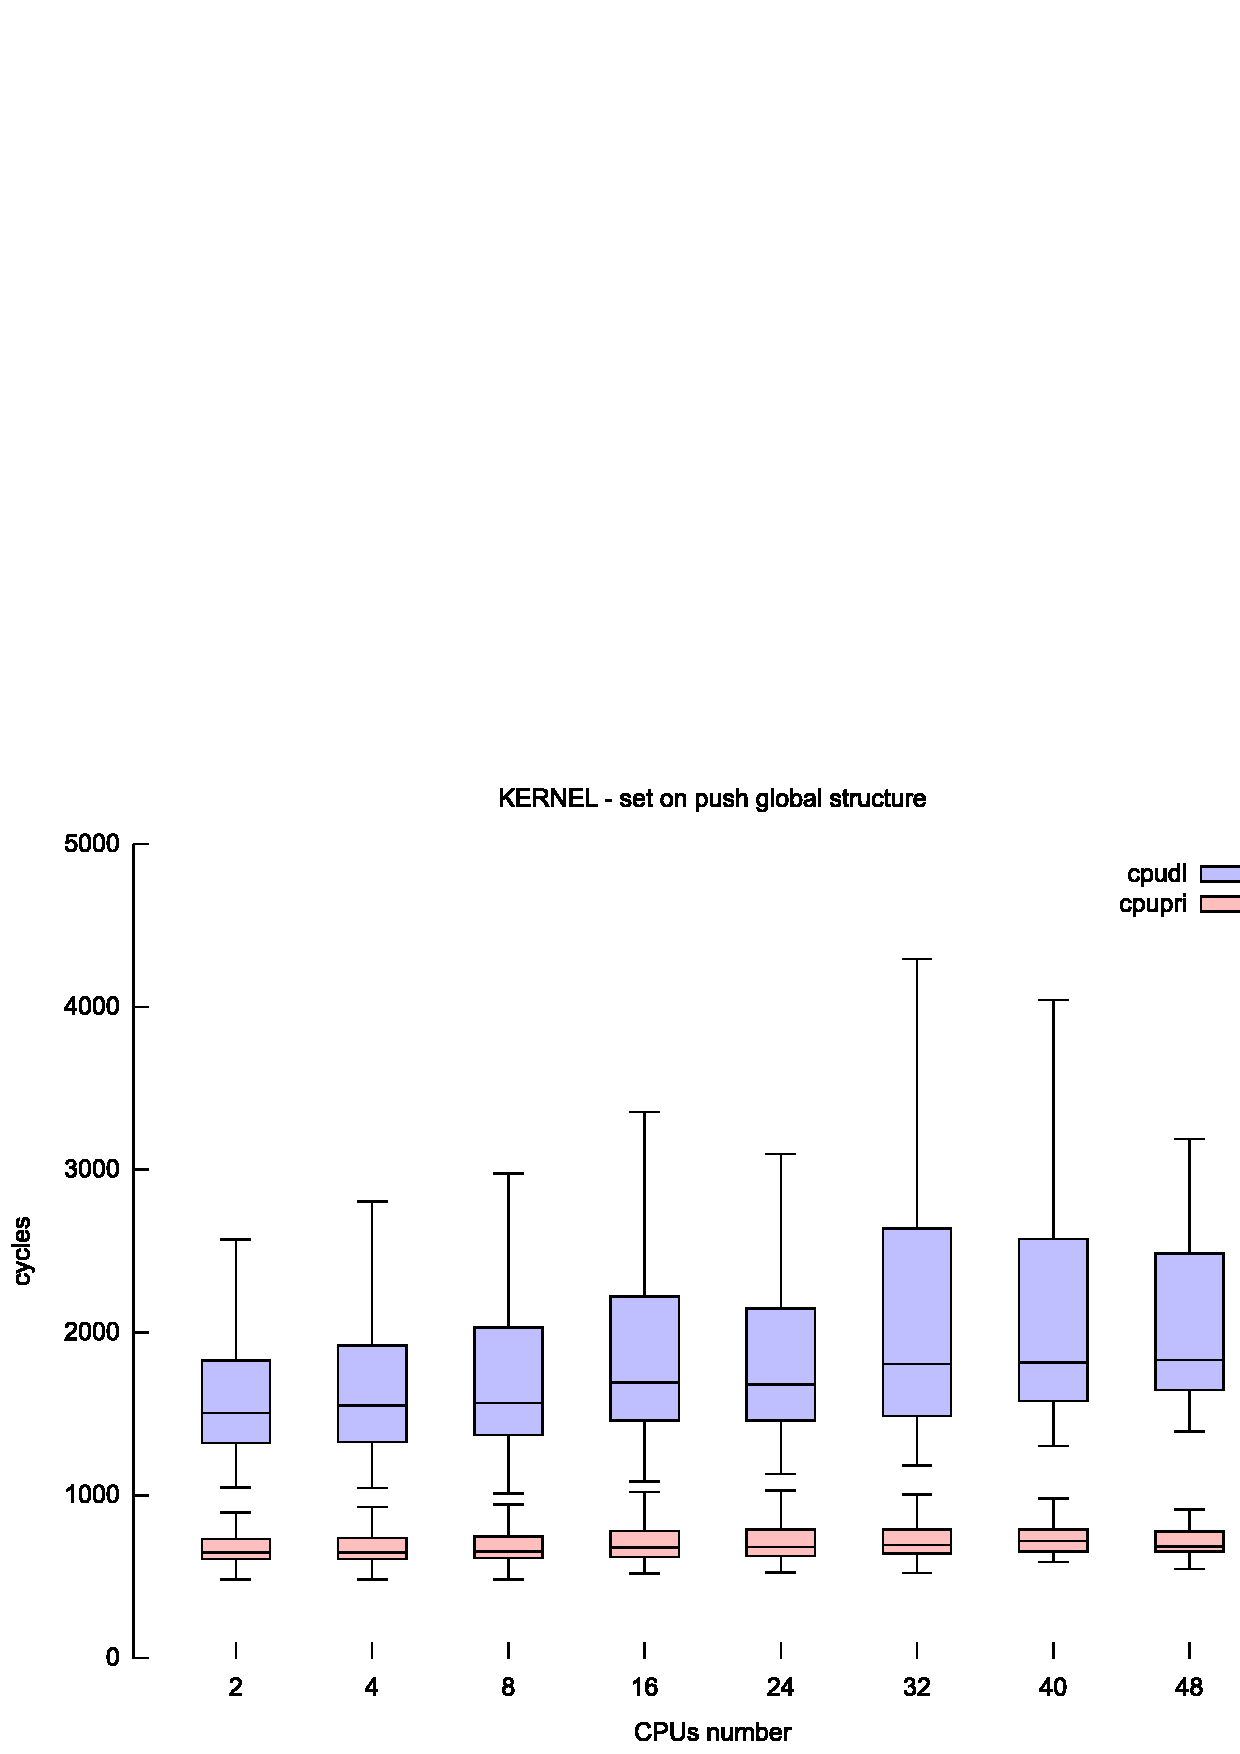
\includegraphics[height=3.5in, keepaspectratio]{images/kernel_set.pdf}
	\caption{Global data structure modify}
	\label{fig:kernel-set}
\end{figure}

\begin{figure}[htbp]
	\centering
	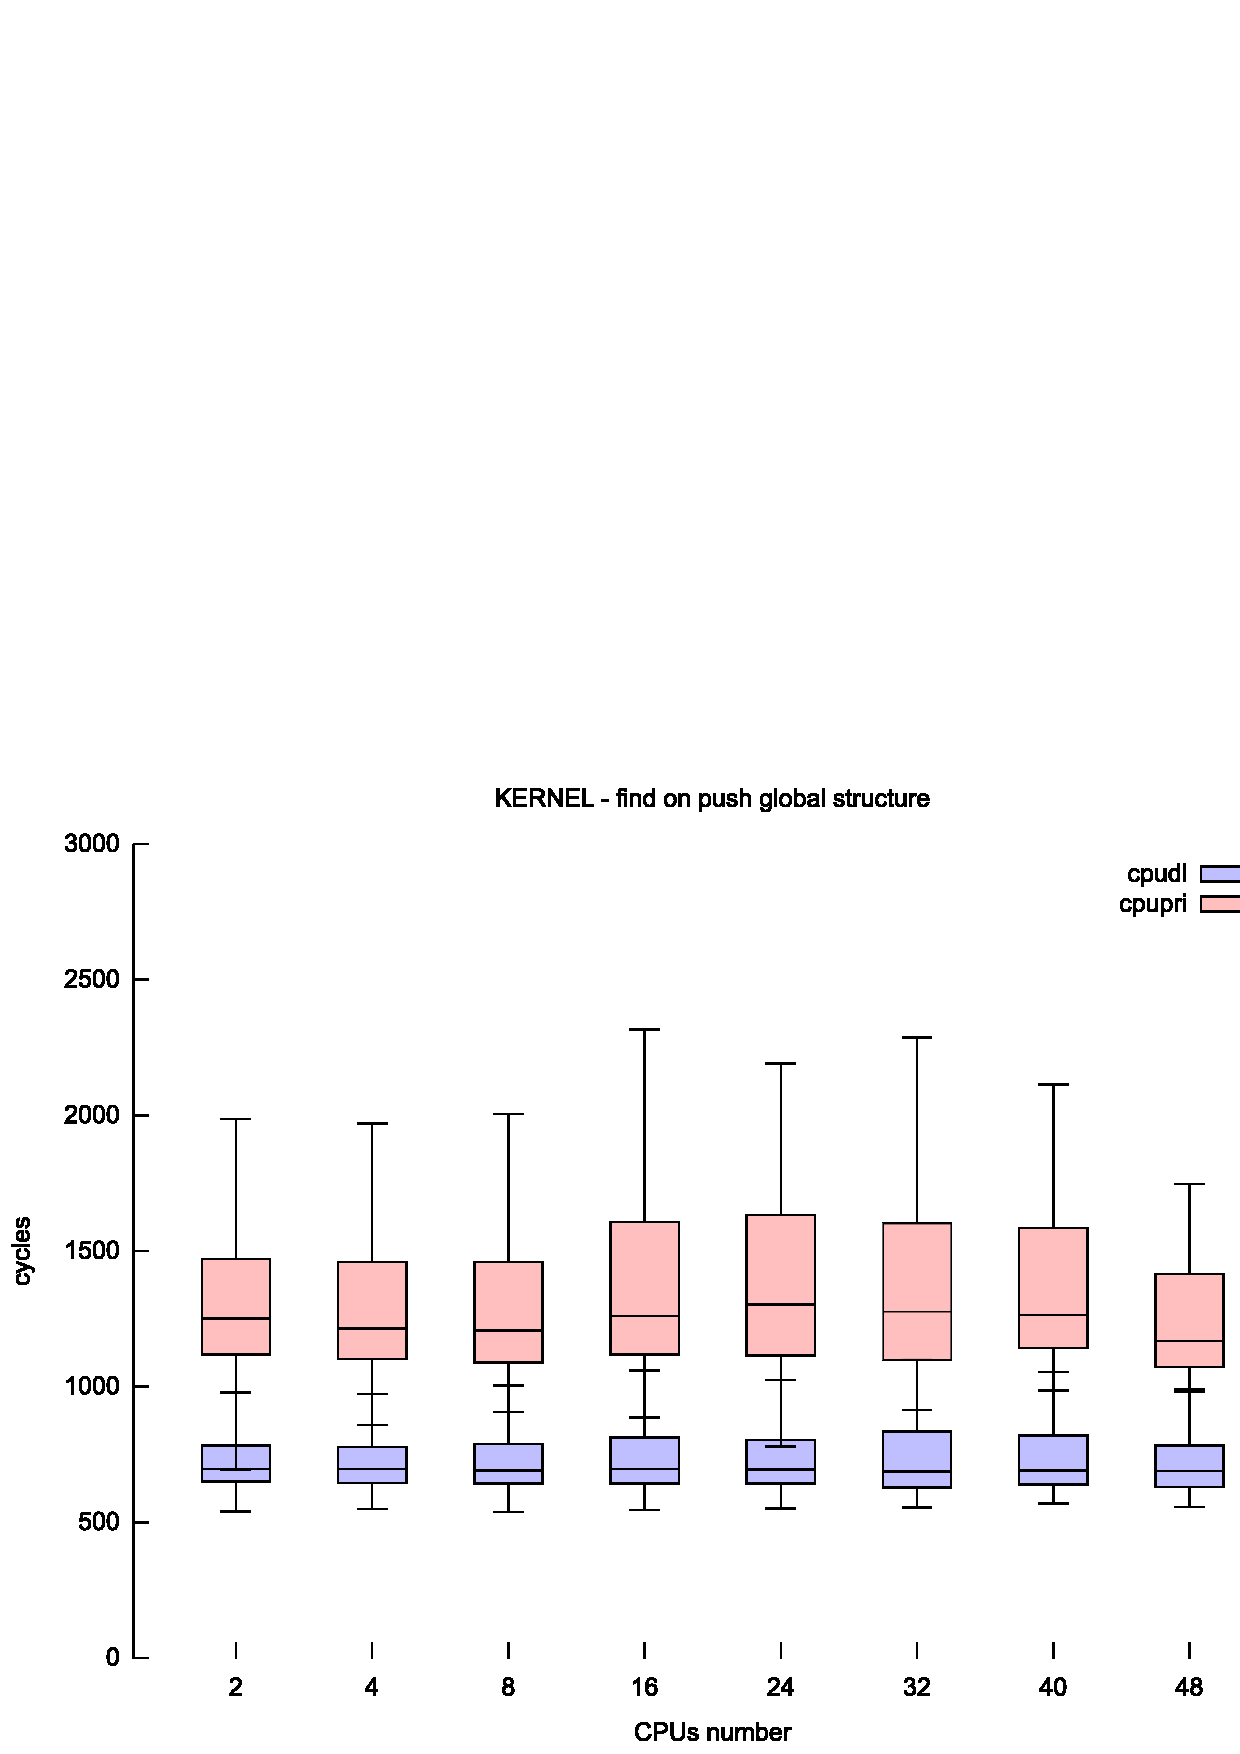
\includegraphics[height=3.5in, keepaspectratio]{images/kernel_find.pdf}
	\caption{Global data structure query}
	\label{fig:kernel-find}
\end{figure}

The figures show the number of cycles (y axis) measured for different number of processors
ranging from 2 to 48 (x axis). The measures are shown in boxplot format: a box indicates all
data comprised between the 25\% and the 75\% percentiles, whereas an horizontal lines 
indicates the median value; also, the vertical lines extend from the minimum to the maximum
value.

In PRACTISE we run the same experiments. As depicted in Section~\ref{sec:PRACTISE_event_gen}
random scheduling events generation is instead part of PRACTISE. We varied the number of
active processors from 2 to 48 as in the former case.

We set the following parameters: 10 milliseconds of thread cycle; 20\% probability of new
arrival; 10\% probability of finish earlier than deadline (for \emph{cpudl} data structure)
or runtime (for \emph{cpupri} data structure); 70\% probability of doing nothing. These
probability values lead to rates of about 20 task activation / (core * s), and 20 task blocking
/ (core * s).

The results are shown in Figures \ref{fig:practise-set-rm} and \ref{fig:practise-set-edf} 
for modifying the \emph{cpupri} and \emph{cpudl} data structures, respectively; and in 
Figures \ref{fig:practise-find-rm} and \ref{fig:practise-find-edf} for querying the \emph{cpupri} 
and \emph{cpudl} data structures, respectively.

\begin{figure}[htbp]
	\centering
	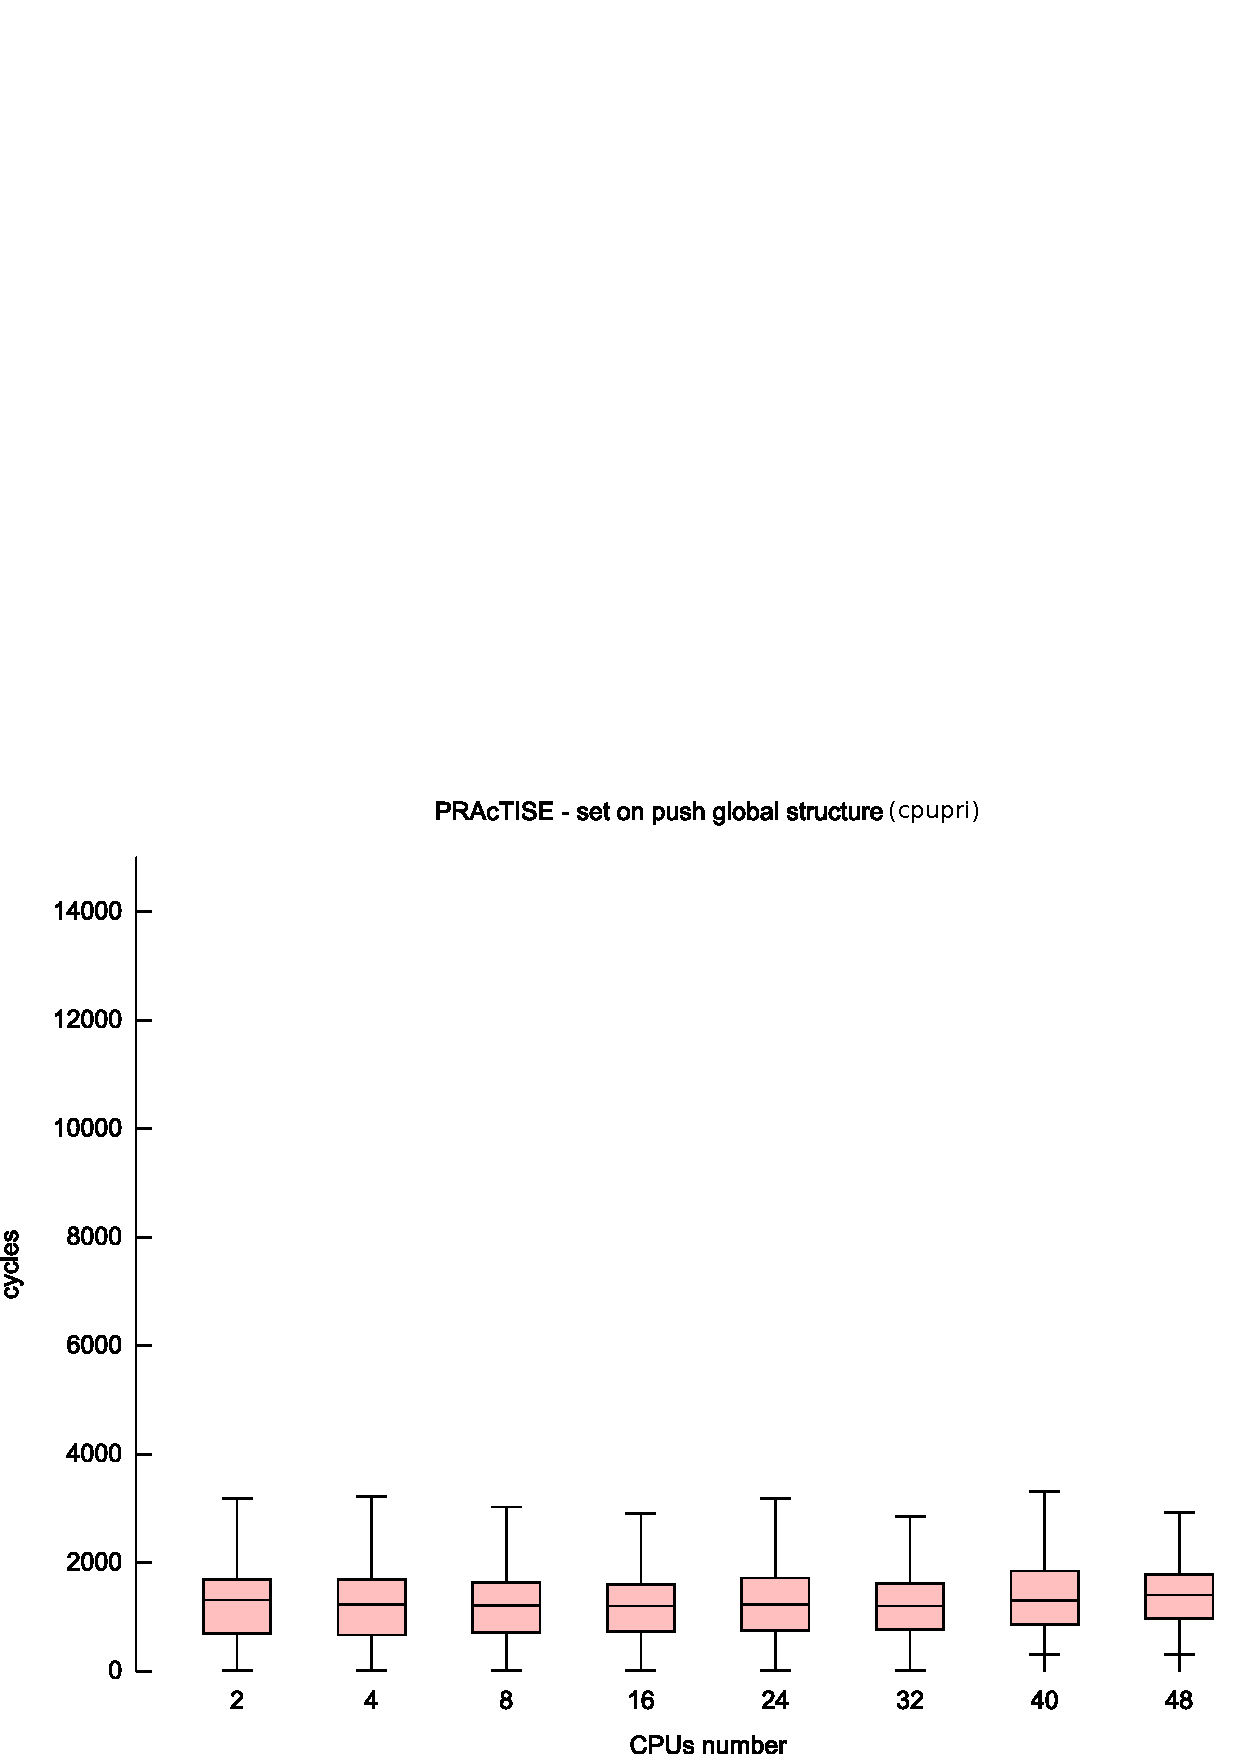
\includegraphics[height=3.5in, keepaspectratio]{images/PRACTISE_set_cpupri.pdf}
	\caption{Global data structure \emph{cpupri} modify}
	\label{fig:practise-set-rm}
\end{figure}

\begin{figure}[htbp]
	\centering
	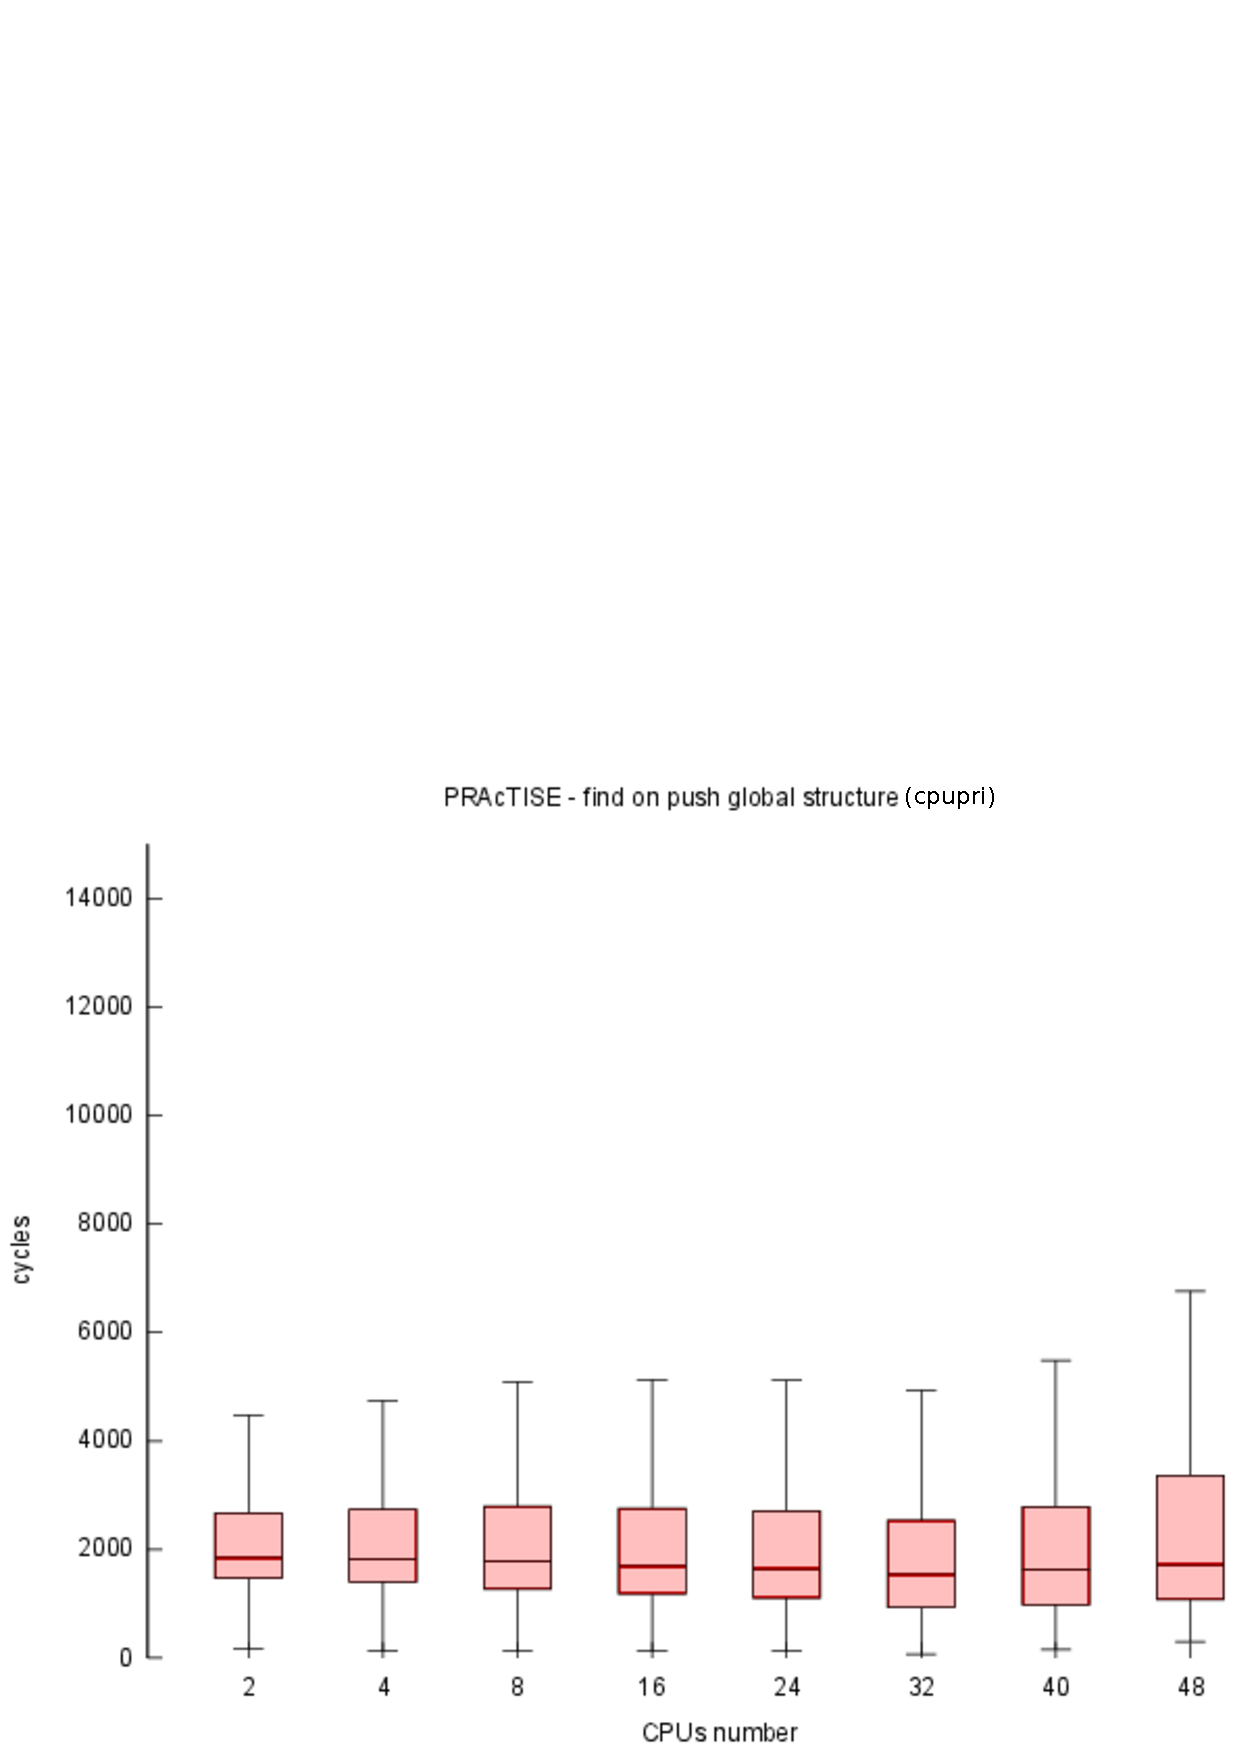
\includegraphics[height=3.5in, keepaspectratio]{images/PRACTISE_find_cpupri.pdf}
	\caption{Global data structure \emph{cpupri} query}
	\label{fig:practise-find-rm}
\end{figure}

\begin{figure}[htbp]
	\centering
	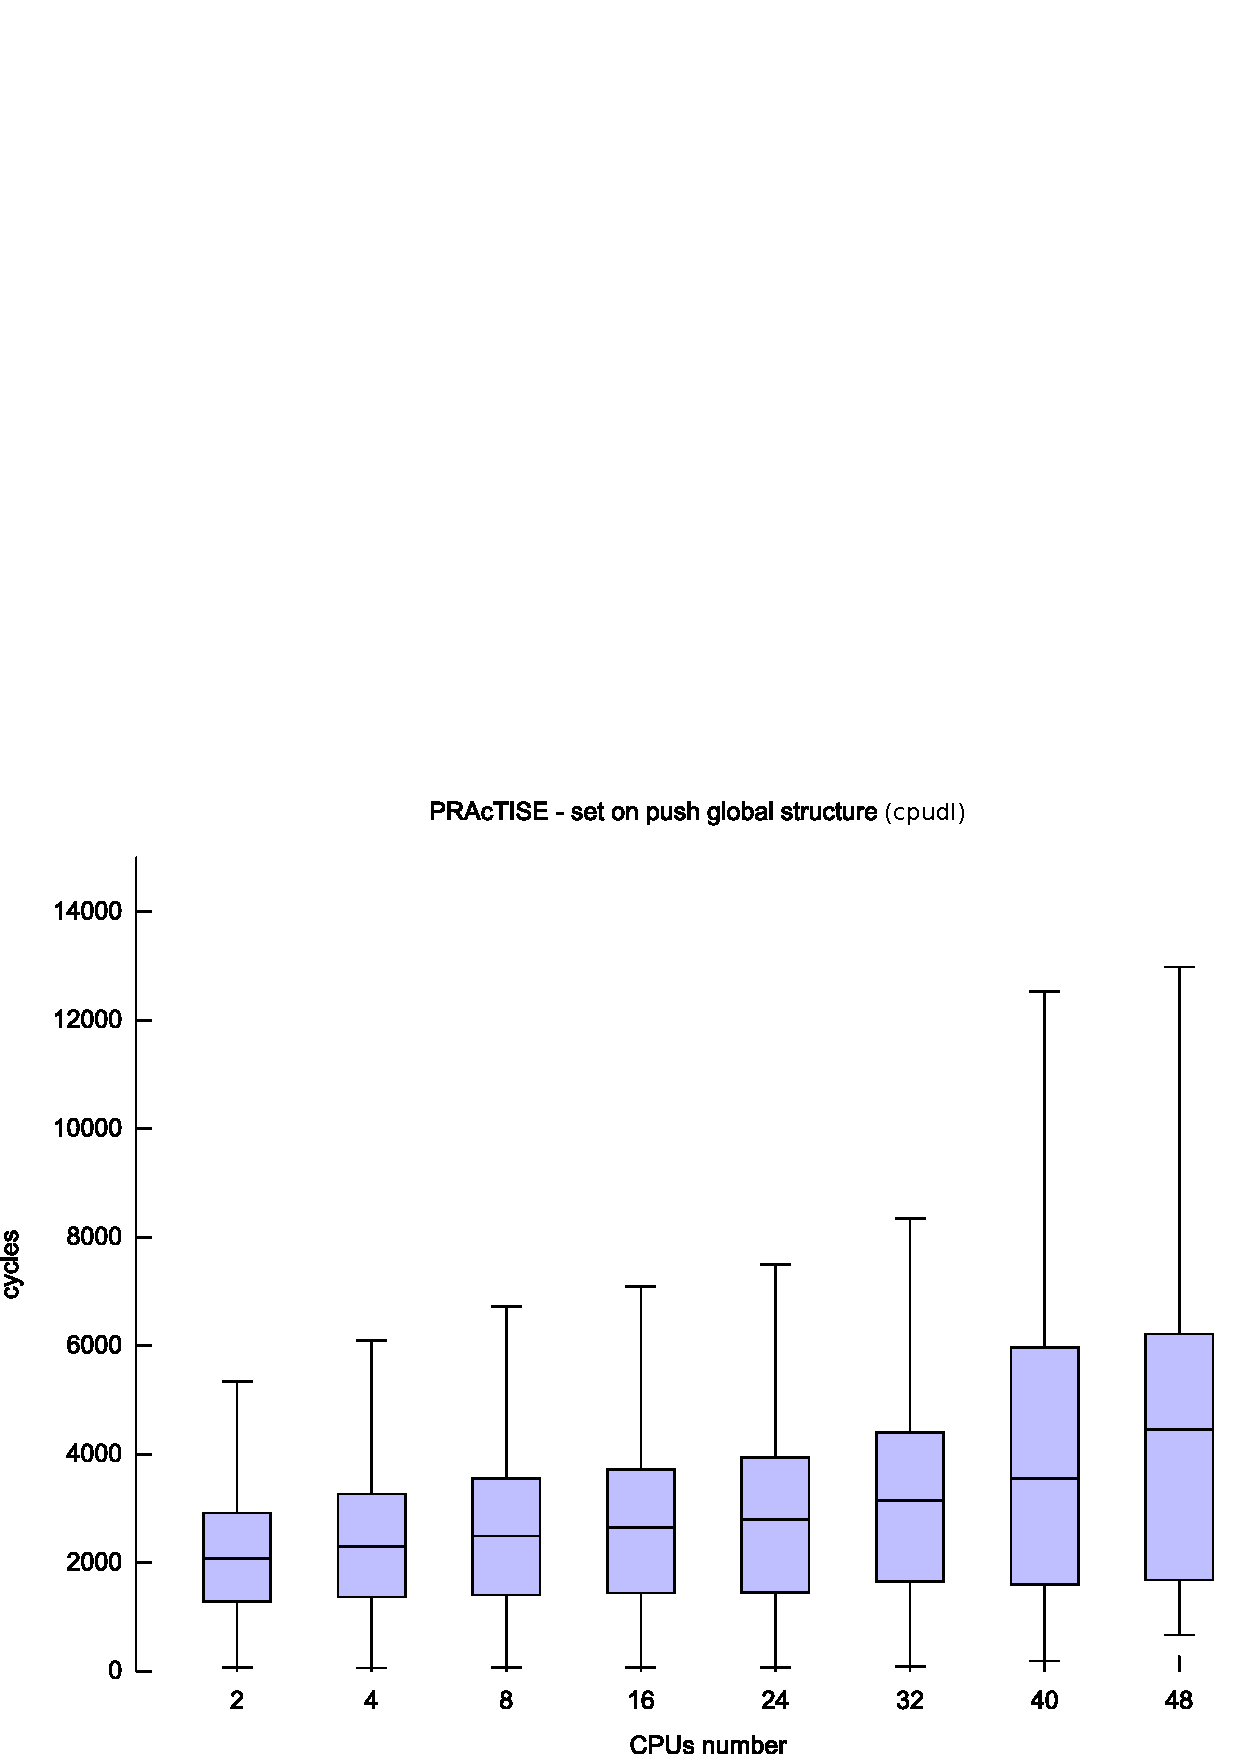
\includegraphics[height=3.5in, keepaspectratio]{images/PRACTISE_set_cpudl.pdf}
	\caption{Global data structure \emph{cpudl} modify}
	\label{fig:practise-set-edf}
\end{figure}

\begin{figure}[htbp]
	\centering
	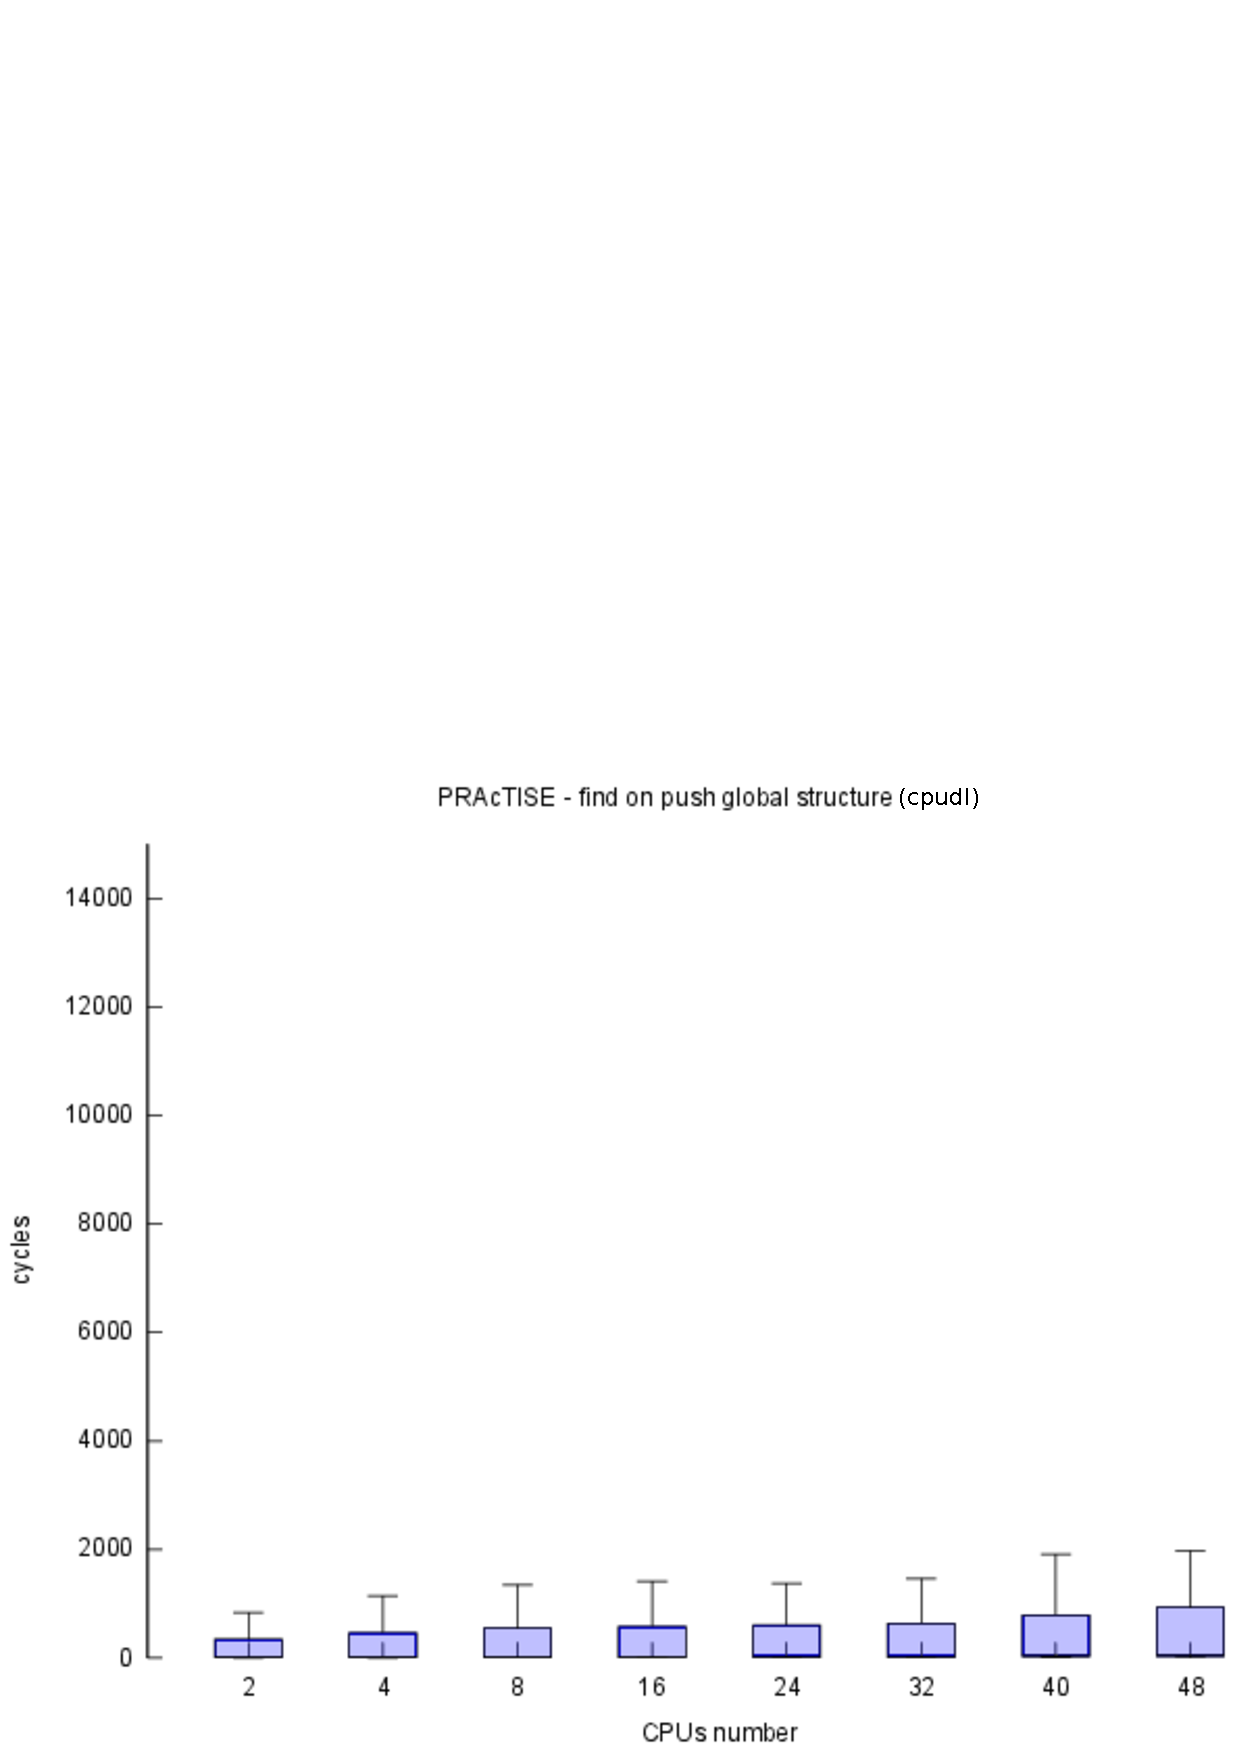
\includegraphics[height=3.5in, keepaspectratio]{images/PRACTISE_find_cpudl.pdf}
	\caption{Global data structure \emph{cpudl} query}
	\label{fig:practise-find-edf}
\end{figure}

Insightful observations can be made comparing performance figures for the same operation
obtained from the kernel and from simulations. Looking at Figure~\ref{fig:kernel-set} we
see that modifying the \emph{cpupri} data structure is generally faster than modifying
\emph{cpudl} data structures: every measure corresponding to the former structure falls
below 1000 cycles while the same operation on \emph{cpudl} takes about 2000 cycles. Same
trend can be noticed in Figures \ref{fig:practise-set-rm} and \ref{fig:practise-set-edf}.
Points dispersion is generally a bit higher than in the previous cases; however median
values for \emph{cpupri} are strictly below 2000 cycles while \emph{cpudl} never goes
under that threshold. We can see that PRACTISE overestimates this measures: in Figure
\ref{fig:practise-set-rm} we see that the estimation for the \emph{set} operation on
\emph{cpupri} are about twice the ones measured in the kernel; however, the same happens
for \emph{cpudl} (in Figure~\ref{fig:practise-set-edf}); therefore, the relative
performance of both does not change.

Regarding query operations the ability of PRACTISE to provide an estimation of actual
trends is even more evident. Figure~\ref{fig:practise-find-edf} shows that a \emph{find} 
on \emph{cpudl} is generally more efficient than the same operation on \emph{cpupri}; this
was expected, because the former simple reads the top element of the heap. Comparing
Figure~\ref{fig:practise-find-rm} with Figure~\ref{fig:practise-find-edf} we can state 
that latter operations are the most efficient also in the simulated environment.
As a concluding use-case, it is worth mentioning that PRACTISE has already been used as a
testing environment for the last SCHED\_DEADLINE release on the LKLM\footnote{LKLM 
(Linux Kernel Mailing List) thread available at: \url{https://lklm.org/lklm/2012/4/6/39}}.
The \emph{cpudl} global data structure underwent major changes that needed to be verified.
The tested code has been finally merged within the patch set.

\section{Kernel Experiments\label{sec:exp_setup}}

Regarding the kernel experiments, since the results for the different values 
of CPU utilization are very similar, in the subsequent sections we are 
going to show only the graphs related to task sets with a U value of 0.8.

We will focus on the graphs related to the performance of the \texttt{cpudl} data
structures, that is: the CPU cycles of the \emph{find} operation and the \emph{set}
operation. We will show the number of \emph{push} and \emph{pull} 
operations and we will point out the benefit of using a \texttt{cpudl} data structure
to speed up the pull operations.

\section{Comparison between max-heap and skip list\label{sec:heap_vs_skiplist}}

In this section we are going to focus on the \emph{push} operation: we will compare
the \texttt{cpudl} max-heap with the skip list one.

The results are shown in Figure~\ref{fig:heap_skiplist_find}. 

We can see that the \emph{find} operation is always faster in the skip list
implementation: the median value is always under 600 CPU cycles, while the max-
heap never goes under that threshold. Both implementations are not affected by
the increase in the CPUs number: we can see that the results are the same from
2 to 48 CPUs. This shows that they are both scalable.

\begin{figure}[htbp]
    \includegraphics[width=\columnwidth]{images/heap_skiplist_find.pdf}
    \caption{\emph{set} operation on max-heap and skip list kernel}
    \label{fig:heap_skiplist_find}
\end{figure}

Regarding the \emph{set} operation, the result is reversed 
(Figure~\ref{fig:heap_skiplist_set}): we
see that the max-heap is very fast and never exceeds the 2000 cycles threshold.
We can see that also the scalability of this solution is good: as the number of
CPUs increases, the heap still performs quite well, even if a slight worsening
can be noted when the CPUs are 24 or more.

\begin{figure}[htbp]
    \includegraphics[width=\columnwidth]{images/heap_skiplist_set.pdf}
    \caption{\emph{find} operation on max-heap and skip list kernel}
    \label{fig:heap_skiplist_set}
\end{figure}

The skip list implementation is not as fast as the heap in updating the
structure: the number of CPU cycles needed to perform the same operations are
about double. Regarding the scalability, we can see that the operation tends
to slightly slow while the CPUs are more than 16, but still mantains
a good performance even with 48 CPUs.

To perform a fair comparison between the two implementations, we need to know
the number of operations carried out on the data structure. 
In Figure~\ref{fig:heap_skiplist_nr_set} 
and Figure~\ref{fig:heap_skiplist_nr_find} we can see the number of \emph{set} 
and \emph{find} per CPU operations, respectively. Since the number of \emph{set} 
operations greatly exceeds the \emph{find}
one, and since the spread between max-heap and skip list performance is much
wider in the \emph{set} case than the \emph{find} one, we can definitely
state that the heap is a better solution for the \emph{push} operation.

\begin{figure}[htbp]
    \includegraphics[width=\columnwidth]{images/heap_skiplist_nr_push_set}
    \caption{\emph{set} operations number}
    \label{fig:heap_skiplist_nr_set}
\end{figure}

\begin{figure}[htbp]
    \includegraphics[width=\columnwidth]{images/heap_skiplist_nr_push_find}
    \caption{\emph{find} operations number}
    \label{fig:heap_skiplist_nr_find}
\end{figure}

\section{Improved Pull algorithm performance\label{sec:improved_pull_perf}}

As we have seen in Section~\ref{sec:pull_dl_impl} and in Section~\ref{sec:pull_algo}, 
the current implementation of \texttt{SCHED\_DEADLINE} lacks a data structure 
to speed up the pull operation. So, we decided to address this problem following 
the same approach developed for the push operation. We chose the skip list 
implementation of the \texttt{cpudl} data structure and, with a kernel modified
as such, we conduct the same experiments described in Section~\ref{sec:PRACTISE_exp_setup}.\\
The results are shown in Figure~\ref{fig:cpudl_pull_nr_pushed_away} and in 
Figure~\ref{fig:cpudl_pull_nr_pulled_here} where we can see
the number of succesfull per-CPU task migrations due to push and pull operations,
respectively. Regarding the push-related migrations, we see that there is
no difference; on the other hand, since we used a \texttt{cpudl}
data structure also for \emph{pull} operation, there is no need to 
explore all runqueues in the system: so, the number of migrations is lower
for every number of online CPUs.

\begin{figure}[htbp]
    \includegraphics[width=\columnwidth]{images/cpudl_pull_nr_pushed_away}
    \caption{Number of task migrations due to push operation}
    \label{fig:cpudl_pull_nr_pushed_away}
\end{figure}

\begin{figure}[htbp]
    \includegraphics[width=\columnwidth]{images/cpudl_pull_nr_pulled_here}
    \caption{Number of task migrations due to pull operation}
    \label{fig:cpudl_pull_nr_pulled_here}
\end{figure}

\section{Bitmap flat combining performance\label{sec:bm_fc_perf}}

In this section we discuss the performance of
the bitmap flat combining solutions. This implementation is the basis
for the fastcache algorithm.

In Figures~\ref{fig:bm_fc_push} and \ref{fig:bm_fc_pull} we can observe 
the performance related to the push and the pull operations, respectively.
Each graphs contains two figures: the \emph{find} operation 
results on the top half and the \emph{set} operation results
on the bottom half.

\begin{figure}[htbp]
    \includegraphics[width=\columnwidth]{images/bm_fc_push}
    \caption{Bitmap flat combining push performance}
    \label{fig:bm_fc_push}
\end{figure}

\begin{figure}[htbp]
    \includegraphics[width=\columnwidth]{images/bm_fc_pull}
    \caption{Bitmap flat combining pull performance}
    \label{fig:bm_fc_pull}
\end{figure}

Regarding the push operation, we compared the bitmap flat combining
with the best current solution: the max-heap. We can see that,
as with the skip list, flat combining reaches very high performance in
the \emph{find} operation. This is due to the best CPU cached value:
if the cache is valid, we can immediately return that CPU index, so
the operation is very fast. The \emph{set} operation is instead slower
for the bitmap flat combining solution. More importantly, we can see
that the performance doesn't scale as well as with the max-heap:
with an increasing number of CPUs, the spread between the two solutions
is even more evident. With 48 online CPUs, the bitmap flat combining
overcomes the 4000 CPU cycles threshold, while the max-heap remains
under 2000 CPU cycles.

Regarding the pull operation, the trend is the same for both \emph{find}
and \emph{set} operations. Here we have to point out that the comparison
is done with the skip list as the improved pull algorithm has been tested
with such data structure.

In conclusion, we see how the cache mechanism, initially introduced
to keep the \emph{cpudl} updated among the underlying runqueues status,
makes the solution very fast for the \emph{find} operation, however, the
flat combining framework is not adequate for the \emph{set} operation.
If we consider the results for the single-lock skip list another time,
we can see how flat combining is even worse than that. This means that
the underlying mechanism to defer work on the data structure puts a non
negligible overhead.

\begin{figure}[htbp]
    \includegraphics[width=\columnwidth]{images/bm_fc_pushed_away}
    \caption{Number of successfull push operations}
    \label{fig:bm_fc_pushed_away}
\end{figure}

Another insightful observation can be made referring to 
Figure~\ref{fig:bm_fc_pushed_away},
where the number of successfull per CPU push operations is showed. In the
graph the max-heap and the flat combining are compared. As we can see,
the latter has a lower number of succesfull migrations: since we
did not change the push mechanism, then the work
deferring mechanism is the responsible. Hence, the data structure 
cannot correctly represents the runqueues status under certain conditions.
This is a notable drawback that highlights the inadequacy of this
implementation.

\section{Fastcache performance\label{sec:fastcache_perf}}

As discussed in the previous sections, a good solution that aims at
speeding up the task migration mechanism, has to achieve very high performance
in the \emph{set} operation. We have seen how the cache introduced
with flat combining offers good performance in the \emph{find} operation,
but the way this cache is filled after being invalidated overcomes that
benefit. With fastcache	(see Section~\ref{sec:Fastcache}), we try to focus on the cache mechanism,
refilling that with a very light-weight algorithm while ensuring that
the \emph{set} operation related work will be done immediately.

In Figure~\ref{fig:fastcache_push} we can see the performance of
the \emph{find} (top half) and \emph{set} (bottom half) push related
operations.

\begin{figure}[htbp]
    \includegraphics[width=\columnwidth]{images/fastcache_push}
    \caption{Fastcache push performance}
    \label{fig:fastcache_push}
\end{figure}

As usual, we compare fastcache with the max-heap, the fastest solution
for the push operation. As we can see, fastcache overcomes the previous
algorithm, both in the \emph{find} and the \emph{set} operations. The graph related
to the latter operation is the most important: we can see that the trend
remains flat as the number of the CPUs increases. In fact, the spread
between the two graphs is more and more evident increasing the number
of CPUs. Considering the 48 CPUs results, we can see how fastcache
performs the \emph{set} operation in about 600 CPU cycles, while the max-heap
takes more then the 1500 CPU cycles.

The results for the pull operation, showed in Figure~\ref{fig:fastcache_pull},
are quite similar: we see how fastcache, compared to the skip list, 
tends to be always faster.

Also here we can see that the trend of the \emph{set} operation is not 
as flat as the analogous one for push. This phenomenon can be explained 
looking at the number of successfull migration due to push and pull, 
respectively, as shown in Figures~\ref{fig:fastcache_pushed_away} and 
\ref{fig:fastcache_pulled_here}.

\begin{figure}[htbp]
    \includegraphics[width=\columnwidth]{images/fastcache_pull}
    \caption{Fastcache pull performance}
    \label{fig:fastcache_pull}
\end{figure}

We can see that the number of task migrations 
due to the push operation, presented in the former figure, greatly overcomes 
the pull related one, in the latter figure.

\begin{figure}[htbp]
    \includegraphics[width=\columnwidth]{images/fastcache_pushed_away}
    \caption{Number of task migrations due to push operation}
    \label{fig:fastcache_pushed_away}
\end{figure}

\begin{figure}[htbp]
    \includegraphics[width=\columnwidth]{images/fastcache_pulled_here}
    \caption{Number of task migrations due to pull operation}
    \label{fig:fastcache_pulled_here}
\end{figure}

Recall from Figures~\ref{fig:cpudl_push} and \ref{fig:cpudl_pull}
how the push and pull operations work: the former
has to cope with the \texttt{curr} deadline tasks, while the latter keeps
track of the \texttt{next} deadline tasks. This means that is easier, for
the pull \texttt{cpudl} data structure, to have an higher number of empty
items: that is, CPUs with no \texttt{next} deadline tasks. This condition
leads to an higher percentage of \emph{set} operations with the flag
\texttt{is\_valid} set to zero, thus an higher percentage of cache
invalidations. Since the slow path has to be followed more frequently for
the pull related \emph{set} operation, fastcache tends to be slightly dependent 
on the number of underlying CPUs. However, we can see that with an higher
number of CPUs fastcache performs better than the skip list. So we can state 
that fastcache scales better than the skip list.

Finally, from these latest figures, we can see that the number of task
migrations is about the same for max-heap, skip list and fastcache.


% conclusions
\chapter{Conclusions and Future Work}\label{chap:conclusions}

In this thesis, we presented PRACTISE a tool for performance analysis and
testing of real-time multicore schedulers for the Linux kernel.
PRACTISE enables fast prototyping of real-time multicore scheduling
mechanisms, allowing easy debugging and testing of such mechanisms in
user-space.
We showed the ability of this novel framework to predict the relative 
performance of multiple solutions.

Thanks to PRACTISE we were able to develop a set of innovative solutions
to manage the task migrations in \texttt{SCHED\_DEADLINE} scheduling class.
We started with a probabilistic data structure, the skip list, that performs
very well in \emph{find} operation. Then we developed a specific implementation
of the flat combining framework, named bitmap flat combining. This algorithm
performs even better than the skip list in \emph{find} operation. However,
we showed that bitmap flat combining is not suitable for task migration mechanism.
Finally, we developed fastcache, a novel algorithm that overcomes all previous
one.

Regarding PRACTISE, a lot of improvements can be made.

First, it is possible to refine the framework adherence to the Linux kernel.
In doing so, we have to enhance task affinity management, local runqueues
capabilities and provide the possibility to generate random scheduling events
following probability distributions gathered from real task sets execution
traces. Moreover, an improvement to the \emph{performance analysis} mode can be
made. In particular, the main goal
is to alleviate the unpredictable latency introduced by a preemptive kernel
while the user space code is under measure. A possible solution
is first to develop some scripts that can translate the code in the
kernel space equivalent one. After that, it will be possible to run that
code inside PRACTISE, if the tool will be designed to work as a kernel
module. Doing so, it will be possible to obtain more control on kernel
preemption so as to obtain more accurate measurements.

Thanks to PRACTISE, we developed a set of improved solutions for the
\emph{cpudl} data structure. Driven by PRACTISE results, we decided
to port each one of them in kernel space. The results show that, thanks to
the \emph{fastcache} algorithm, the task migration latency
has been reduced, with a significant improvement from the point of view
of the scalability.

A considerable result has also been obtained with the new pull algorithm:
it has been showed that using a \texttt{cpudl} data structure even in the
pull operation reduces the spurious task migrations, leading to a schedule
closer to the theoretic \emph{G-EDF}.

Regarding those aspects the research is all but over. To better understand
how the schedules imposed by \texttt{SCHED\_DEADLINE} are close to \emph{G-EDF}
a deep analysis is needed: it would be appropriate to develop a tool aimed
to verify, for a given task sets, that the schedule obtained is really
the \emph{G-EDF} one. Driven by this results, it will be possible to
address all cases where a schedule divergency arises.

Finally, the \emph{fastcache} algorithm opens several usage scenarios that
deserve to be investigated. Probably, the most interesting of those is the
implementation of a single global (but scalable) ready queue: this way,
reaching a real \emph{G-EDF} scheduling policy will be plain. 
The original \texttt{SCHED\_RT} scheduling class authors stated that a distributed
runqueues design can scales well compared to a single global runqueue 
one~\cite{molnar07}.
But with the introduction of proper lock-free data structures and algoritms
this statement may no longer be true.


% code listings, etc.
\appendix

\chapter{Code listings}\label{chap:codelst}

\section{\texttt{cpudl} skip list implementation}\label{sec:cpudl_skiplist_code}
\lstinputlisting[language=C, basicstyle=\scriptsize]
{code/skiplist/cpudl.h}
\lstinputlisting[language=C, basicstyle=\scriptsize]
{code/skiplist/cpudl.c}

\section{\texttt{cpudl} bitmap flat combining implementation}\label{sec:cpudl_bm_fc_code}
\lstinputlisting[language=C, basicstyle=\scriptsize]
{code/bmfc/cpudl.h}
\lstinputlisting[language=C, basicstyle=\scriptsize]
{code/bmfc/cpudl.c}
\lstinputlisting[language=C, basicstyle=\scriptsize]
{code/bmfc/bmfc.h}
\lstinputlisting[language=C, basicstyle=\scriptsize]
{code/bmfc/bmfc.c}

\section{\texttt{cpudl} fastcache implementation}\label{sec:cpudl_fastcache_code}
\lstinputlisting[language=C, basicstyle=\scriptsize]
{code/fastcache/cpudl.h}
\lstinputlisting[language=C, basicstyle=\scriptsize]
{code/fastcache/cpudl.c}

\section{Improved pull algorithm}\label{sec:improved_pull_code}
\lstinputlisting[language=C, basicstyle=\scriptsize]
{code/skiplist/dl.c}


\backmatter

\chapter{Acknowledgments}

Vorrei innanzitutto ringraziare il prof. Giuseppe Lipari per avermi dato
l'occasione di svolgere questa tesi. Il suo continuo supporto \`e stato un
fondamentale aiuto per raggiungere il risultato finale.

Desidero ringraziare anche il prof. Paolo Ancilotti per la sua disponibilit\`a
nell'assistermi durante la discussione.

Un ringraziamento particolare va a Juri Lelli. Juri mi ha assistito per
tutta la durata del lavoro, aiutandomi in ogni aspetto tecnico della tesi:
senza la sua grande disponibilit\`a probabilmente non potrei scrivere adesso 
queste parole.

E ora, \`e il momento di ringraziare famiglia ed amici.

Il primo pensiero \`e ``condiviso'' tra mia nonna e Katia. La prima perch\`e
in tutti questi anni non ha mai rinunciato al difficile compito di farmi,
oltre che da nonna, da mamma. Nonna, posso solo dirti che ci sei riuscita
in pieno. La seconda perch\`e ha sempre creduto in me, infodendomi
coraggio, fiducia e serenit\`a anche nei momenti più difficili. Sapere di
averti accanto \`e bellissimo: GRAZIE!
Vorrei inoltre ringraziare mio padre, che ha avuto la pazienza di aspettare
fino ad oggi: spero finalmente di averlo fatto contento con il conseguimento 
del titolo.

Poi, non posso dimenticarmi dei miei amici. Con molti di loro ho avuto
il piacere di studiare insieme: se posso ricordare con un sorriso tutti
i giorni passati in biblioteche ed aule studio, \`e sicuramente grazie a
loro. Fra questi voglio citare il Ture che prima o poi, ne sono sicuro,
riuscir\`a a vendermi una lampada (ma non riuscir\`a mai a battermi ad Hobosoccer);
Enri che \`e il secondo miglior giocatore del mondo di Hobosoccer (complimenti, 
perch\`e il primo \`e di un altro pianeta);
il Tolo, che invece a studiare al CNR non \`e mai venuto; Jacopo, che
condivide con me l'idea del giusto ``metodo'' di studio; Rani, che prima
o poi smetter\`a di usare Windows e di fare pompaggio in panca (o forse no); 
il Fao, costantemente impegnato con
i suoi ``cantieri'' ma che non perde mai occasione per dirmi che sono bravo 
e il Landi, che mi ha insegnato (e mi insegna) tantissimo su tematiche 
extra-universitarie di indubbio interesse.
Per finire l'elenco degli uomini ``duri e puri'' non posso non citare Roberta, che voglio
ringraziare per non avermi usato come merenda durante i pomeriggi di studio.
So che la tentazione \`e stata forte.
Ma un gruppo di soli maschi non fa sugo, e allora ne approfitto per ringraziare
le bellissime del Putignano's Group: Sara l'architetto dal capello corto, 
Serena che devo ringraziare poco perch\`e siamo ``nemici'', Guenda che non riuscir\`a
mai a condurre un mezzo a motore, Francesca che con la guida \`e
messa forse peggio di Guenda, Marghe che probabilmente le batte entrambe, Laura 
che credo non abbia nemmeno la patente ed altre che sicuramente adesso
non ricordo (ma nessuna di queste \`e comunque in grado di guidare).
Infine devo ringraziare Luca, un preziosissimo compagno di studi che ho avuto
il piacere di lasciare indietro (in modo imbarazzante, direi) durante un giro
in moto all'Abetone. Citarlo qui \`e l'ultima risorsa che ho per suscitare il
suo orgoglio e convincerlo a girare ancora con me.


\bibliography{bibliography}
\bibliographystyle{plain}
\end{document}
